%-------------------------------PPT Title-------------------------------------
\title{材料模拟软件与方法简介\rm{(III)}}
%-----------------------------------------------------------------------------

%----------------------------Author & Date------------------------------------
%\author[\textrm{Jun\_Jiang}]{姜\;\;骏\inst{}} %[]{} (optional, use only with lots of authors)
%% - Give the names in the same order as the appear in the paper.
%% - Use the \inst{?} command only if the authors have different
%%   affiliation.
\institute[BCC]{\inst{}%
%\institute[Gain~Strong]{\inst{}%
\vskip -20pt 北京市计算中心~云平台事业部~姜骏}
%\vskip -20pt {\large 格致斯创~科技}}
\date[\today] % (optional, should be abbreviation of conference name)
{	{\fontsize{6.2pt}{4.2pt}\selectfont{\textcolor{blue}{E-mail:~}\url{jiangjun@bcc.ac.cn}}}
\vskip 45 pt {\fontsize{8.2pt}{6.2pt}\selectfont{北京科技大学% 报告地点
	\vskip 5 pt \textrm{2024.04.18}}}
}

%% - Either use conference name or its abbreviation
%% - Not really information to the audience, more for people (including
%%   yourself) who are reading the slides onlin%%   yourself) who are reading the slides onlin%%   yourself) who are reading the slides onlineee
%%%%%%%%%%%%%%%%%%%%%%%%%%%%%%%%%%%%%%%%%%%%%%%%%%%%%%%%%%%%%%%%%%%%%%%%%%%%%%%%%%%%%%%%%%%%%%%%%%%%%%%%%%%%%%%%%%%%%

\subject{}
% This is only inserted into the PDF information catalog. Can be left
% out.
%\maketitle
\frame
{
%	\frametitle{\fontsize{9.5pt}{5.2pt}\selectfont{\textcolor{orange}{“高通量并发式材料计算算法与软件”年度检查}}}
\titlepage
}
%-----------------------------------------------------------------------------

%------------------------------------------------------------------------------列出全文 outline ---------------------------------------------------------------------------------
\section*{}
\frame[allowframebreaks]
{
  \frametitle{Outline}
%  \frametitle{\textcolor{mycolor}{\secname}}
  \tableofcontents%[current,currentsection,currentsubsection]
}
%%在每个section之前列出全部Outline
%%类似的在每个subsection之前列出全部Outline是\AtBeginSubsection[]
%\AtBeginSection[]
%{
%  \frame<handout:0>%[allowframebreaks]
%  {
%    \frametitle{Outline}
%%全部Outline中,本部分加亮
%    \tableofcontents[current,currentsection]
%  }
%}

\small
\section{计算示例:~\rm{VASP}计算}
\subsection{\rm{VASP}的输入与输出文件}\label{Sec:atom-Pt}
%真空中的孤立原子的基态能量是\textrm{VASP}中最简单的算例,通过学习金属\textrm{Pt}原子基态能量的计算,可以掌握典型的\textrm{VASP}的主体流程\footnote{在所有计算之前,请确认\textrm{VASP}软件已经正确安装。},了解体系基态能量最小化的基本算法,并熟悉基本的输入/输出文件的内容。此外,还可以了解如何在已完成计算的基础上,进行计算精度提升或完成后续计算等一系列处理方式。
%\subsection{输入文件}
\frame{
	\frametitle{输入文件}
\textrm{VASP}要求所有的计算都在指定的计算目录下进行%(比如针对当前的算例,可以建目录\textrm{Pt\_atom})。
\begin{itemize}
	\item 准备计算所必需的四个输入文件:~文件名必须是\textcolor{magenta}{\textrm{INCAR}}、\textcolor{magenta}{\textrm{KPOINTS}}、\textcolor{magenta}{\textrm{POSCAR}}和\textcolor{magenta}{\textrm{POTCAR}}
%前三个文件,既可以手动输入也可以通过修改其余计算中的对应文件得到;~\textrm{POTCAR}文件存储的是计算对象构成元素的原子数据,包括具体的原子分波、赝原子分波以及赝势和构造赝势使用的交换-相关泛函等信息。\textrm{VASP}开发组在发布软件时会一并提供全部元素的\textrm{POTCAR}。\footnote{由于历史的原因,习惯上将\textrm{POTCAR}称为赝势文件,但实际上\textrm{POTCAR}文件中包含的内容不仅是原子赝势,还包括原子价电子分波函数和赝分波函数,以及补偿电荷等和赝势、\textrm{PAW}势相关的诸多信息,因此称“数据集(\textrm{Dataset})”更准确.}
	\item \textrm{INCAR}是\textrm{VASP}计算的核心控制文件
\end{itemize}
%\subsubsection{\rm{INCAR}}
对于\textrm{Pt}的计算,\textrm{INCAR}的设置:%如图\ref{Pt_atom:INCAR}所示。
\begin{figure}[h!]
\centering
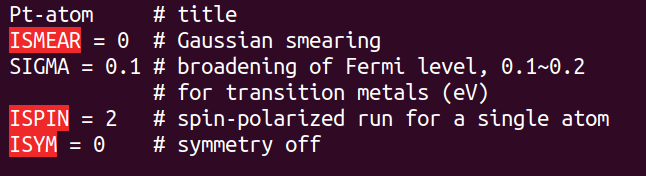
\includegraphics[height=1.00in,width=3.6in,viewport=0 0 480 135,clip]{Figures/Pt_atom-INCAR.png}
\caption{\fontsize{6.2pt}{5.2pt}\selectfont{\textrm{VASP}计算的主要输入控制文件\textrm{INCAR}.}}%(与文献\cite{EPJB33-47_2003}图1对比)
\label{Pt_atom:INCAR}
\end{figure}
对于原子/分子计算,只需要确定少量参数,其余的参数都采用软件推荐的默认值。
}

\frame
{
	\frametitle{\textrm{INCAR}参数}
计算设置的参数,说明如下:~
\begin{itemize}
	\item \textcolor{cyan}{\textit{ISMEAR}}:~设定\textrm{Fermi~}能级的展宽方法
		\vskip 5pt
		{\fontsize{7.2pt}{5.2pt}\selectfont{引入展宽为的是加速收敛
		%本例中参数确定的展宽方法是\textrm{Gaussian}展宽,该方法适用于单原子和局域体系,避免出现\textrm{Fermi}面附近占据数为负值
			。展宽值由参数\textcolor{cyan}{\textit{SIGMA}}确定}}
	\item \textcolor{cyan}{\textit{ISPIN}}:~因为\textrm{Pt}原子的价电子态是$5\mathit{d}^96\mathit{s}^1$,含有未成对电子,因此计算需要考虑自旋极化
	\vskip 5pt
	{\fontsize{7.2pt}{5.2pt}\selectfont{相比于非自旋极化的计算量加倍,即两种自旋(\textrm{spin-up/spin-down})下的电荷密度都要计算}}
	\item \textcolor{cyan}{\textit{ISYM}}:~控制对称性的计算参数%。本次计算中不考虑体系的点群对称性
\end{itemize}
}
%\subsubsection{\rm{KPOINTS}}
\frame
{
	\frametitle{\textrm{KPOINTS}参数}
\textrm{KPOINTS}是描述不可约\textrm{Brillouin}区(\textrm{Irreducible Brillouin Zone,~IBZ})的$\vec k$-点分布的文件%,见图\ref{Pt_atom:KPOINTS}。
\begin{figure}[h!]
\centering
\vskip -5pt
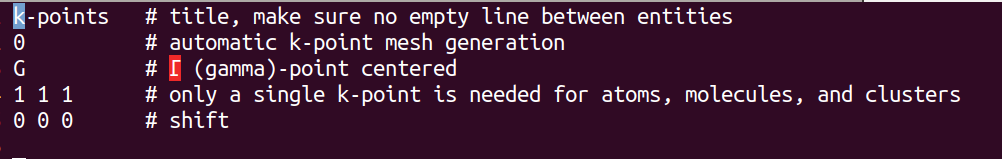
\includegraphics[height=0.60in,width=4.0in, viewport=0 20 750 118,clip]{Figures/Pt_atom-KPOINTS.png}
\caption{\fontsize{6.2pt}{5.2pt}\selectfont{\textrm{VASP}计算的\textrm{IBZ}中的$\vec k$点分布文件\textrm{KPOINTS}.}}%(与文献\cite{EPJB33-47_2003}图1对比)
\label{Pt_atom:KPOINTS}
\end{figure}
因为计算的是单原子体系,无需考虑\textrm{Bloch}定理的影响,因此只需要取一个$\vec k$点($\Gamma$点)
}
%\subsubsection{\rm{POSCAR}}
\frame
{
	\frametitle{\textrm{POSCAR}参数}
\textrm{POSCAR}是描述计算对象结构的文件%,见图\ref{Pt_atom:POSCAR}。
\begin{figure}[h!]
\centering
\vskip -3pt
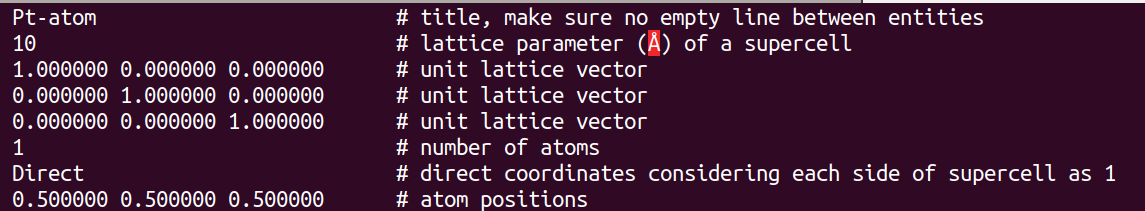
\includegraphics[height=0.70in,width=4.0in,viewport=0 0 850 155,clip]{Figures/Pt_atom-POSCAR.png}
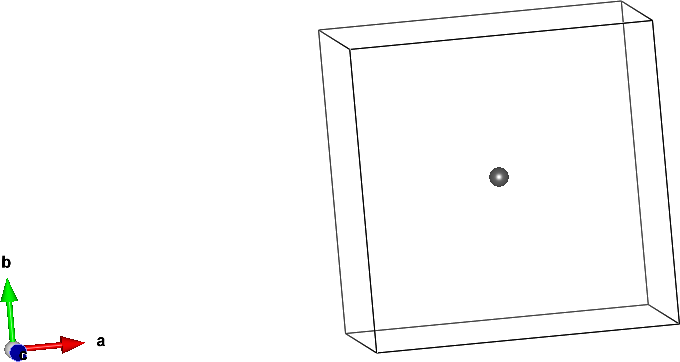
\includegraphics[height=1.2in,width=2.4in,viewport=0 0 680 362,clip]{Figures/Pt_atom-structure.png}
\caption{\fontsize{6.2pt}{5.2pt}\selectfont{\textrm{VASP}计算对象的结构文件\textrm{POSCAR}.}}%(与文献\cite{EPJB33-47_2003}图1对比)
\label{Pt_atom:POSCAR}
\end{figure}
{\fontsize{7.2pt}{5.2pt}\selectfont{\textrm{VASP}中所有的计算对象必须是周期体系,因此对于单原子体系,可以将原子置于一个大的超晶胞($10\times10\times10$)中心,以此确保原子间相互作用足够小}}
}
%\subsubsection{\rm{POTCAR}}
\frame
{
	\frametitle{\textrm{POTCAR}参数}
%\textrm{POTCAR}是计算对象构成元素的数据集文件,包含了\textrm{PAW}计算所需的原子数据,见图\ref{Pt_atom:POTCAR}。本次计算使用\textrm{PAW\_PBE}数据集,是兼顾精度和效率的考虑。\textrm{POTCAR}文件可通过复制\textrm{VASP}提供的原子数据集库中的对应元素数据得到:\\
%\textcolor{magenta}{\textrm{cat~~potcar.PBE.paw/Pt/POTCAR~>~POTCAR}}\\
\begin{figure}[h!]
\centering
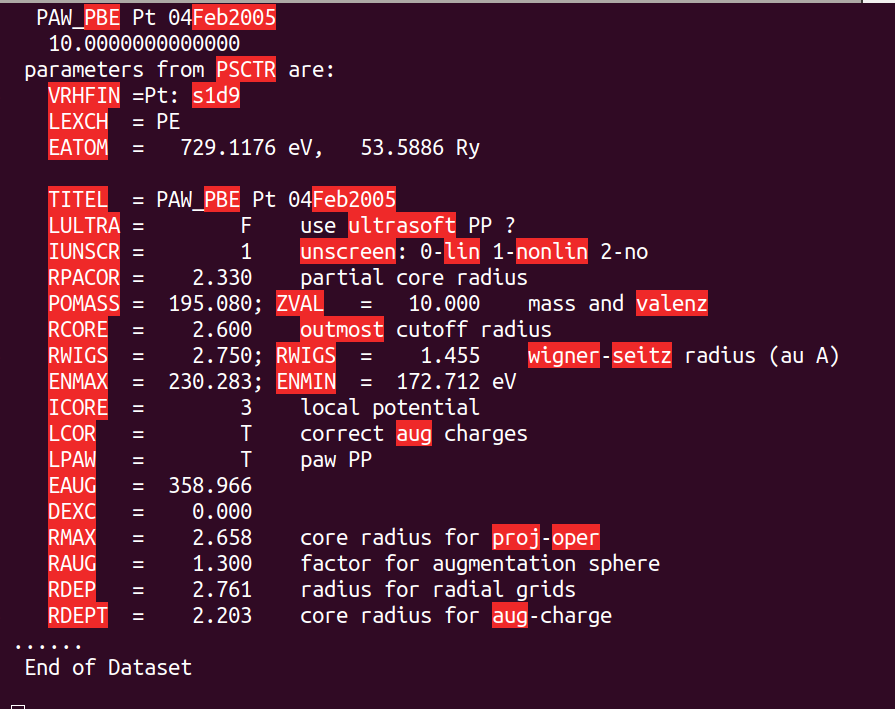
\includegraphics[height=2.7in,width=4.0in,viewport=0 15 780 528,clip]{Figures/Pt_atom-POTCAR.png}
\caption{\fontsize{6.2pt}{5.2pt}\selectfont{\textrm{VASP}计算的原子数据集文件\textrm{POTCAR}.}}%(与文献\cite{EPJB33-47_2003}图1对比)
\label{Pt_atom:POTCAR}
\end{figure}
%注意,这里参数\textit{ENMAX}的值230.283\textrm{eV}将作为计算中能量截断参数\textit{ENCUT}的默认值
}
%\subsection{VASP的运行}
%\textrm{VASP}软件安装在\textrm{Linux}系统环境下,因此在运行\textrm{VASP}的时候需要掌握\textrm{Linux}的一些基本命令。当上节中指定的四个输入文件准备完毕后,只要输入命令:\\
%\textcolor{magenta}{\textrm{VASP\_RUN\_PATH}}\footnote{假设\textrm{VASP}软件正确安装,\textcolor{magenta}{\textrm{VASP\_RUN\_PATH}}表示其可执行文件.}\\
%即可执行,随后屏幕上会有输出,直到计算结束。见图\ref{Pt_atom:runout}。
%\begin{figure}[h!]
%\centering
%%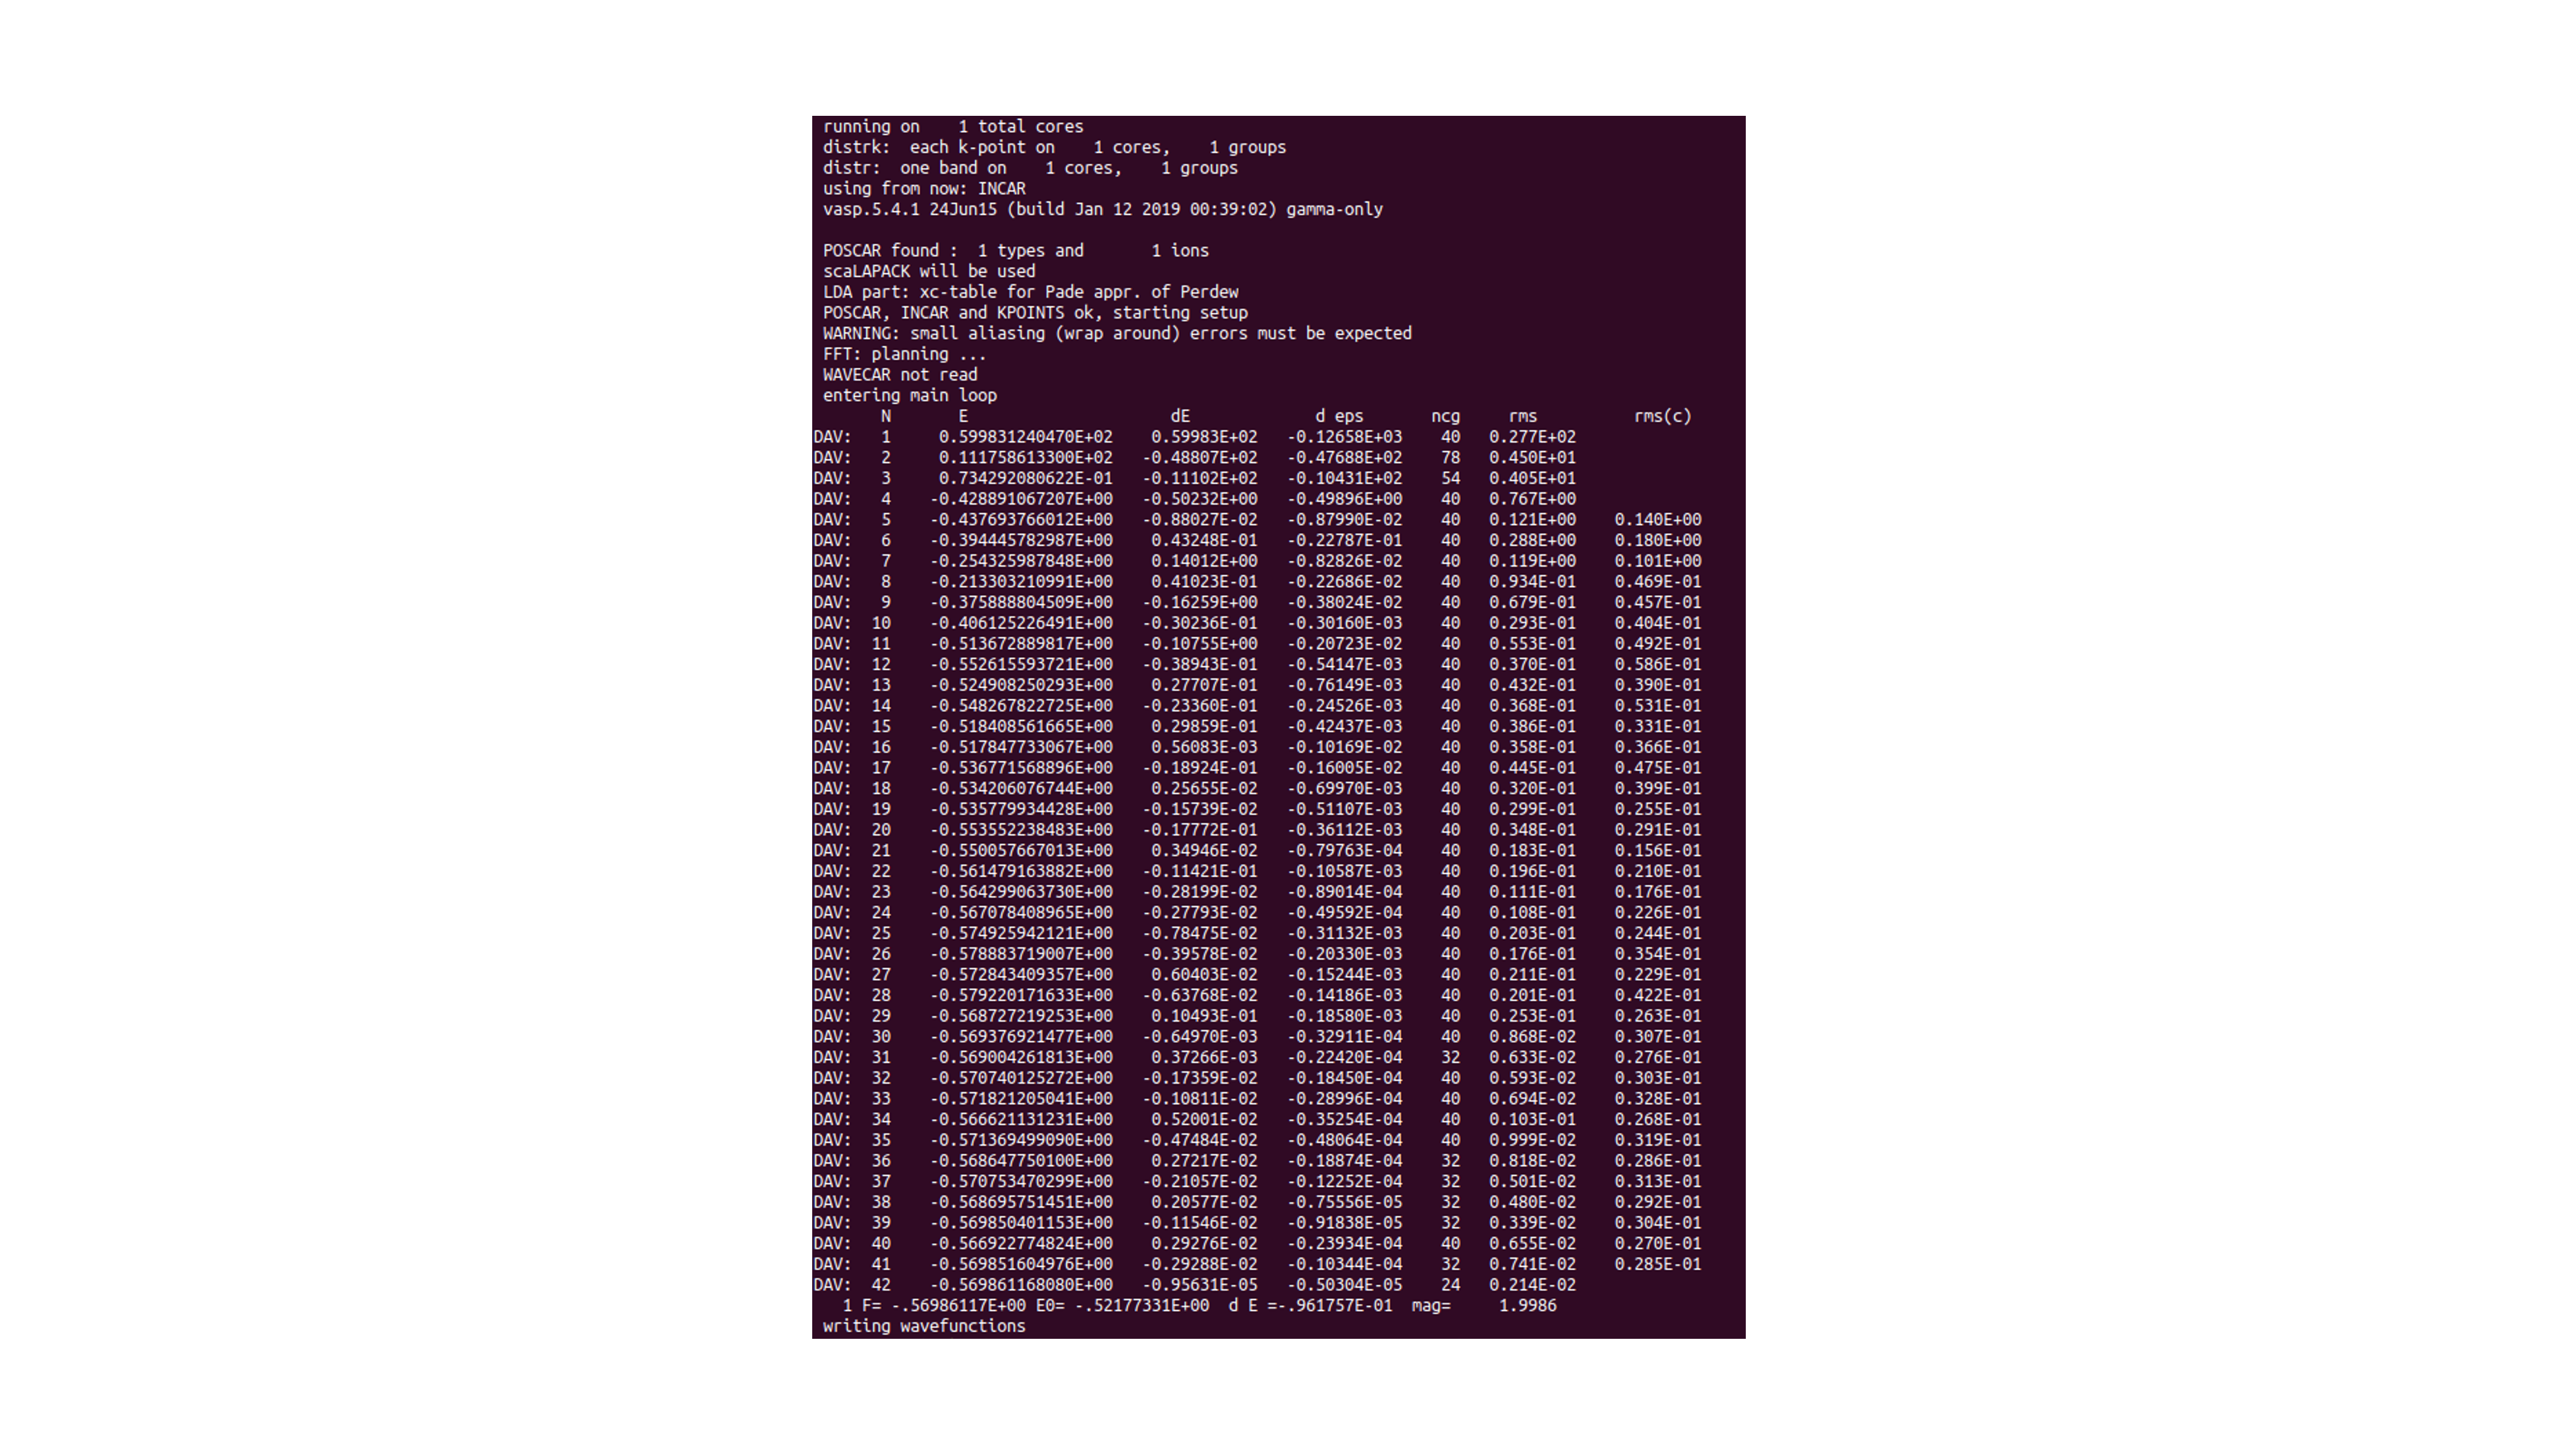
\includegraphics[height=4.5in,width=4.2in,viewport=0 0 780 530,clip]{Pt_atom-runout.png}
%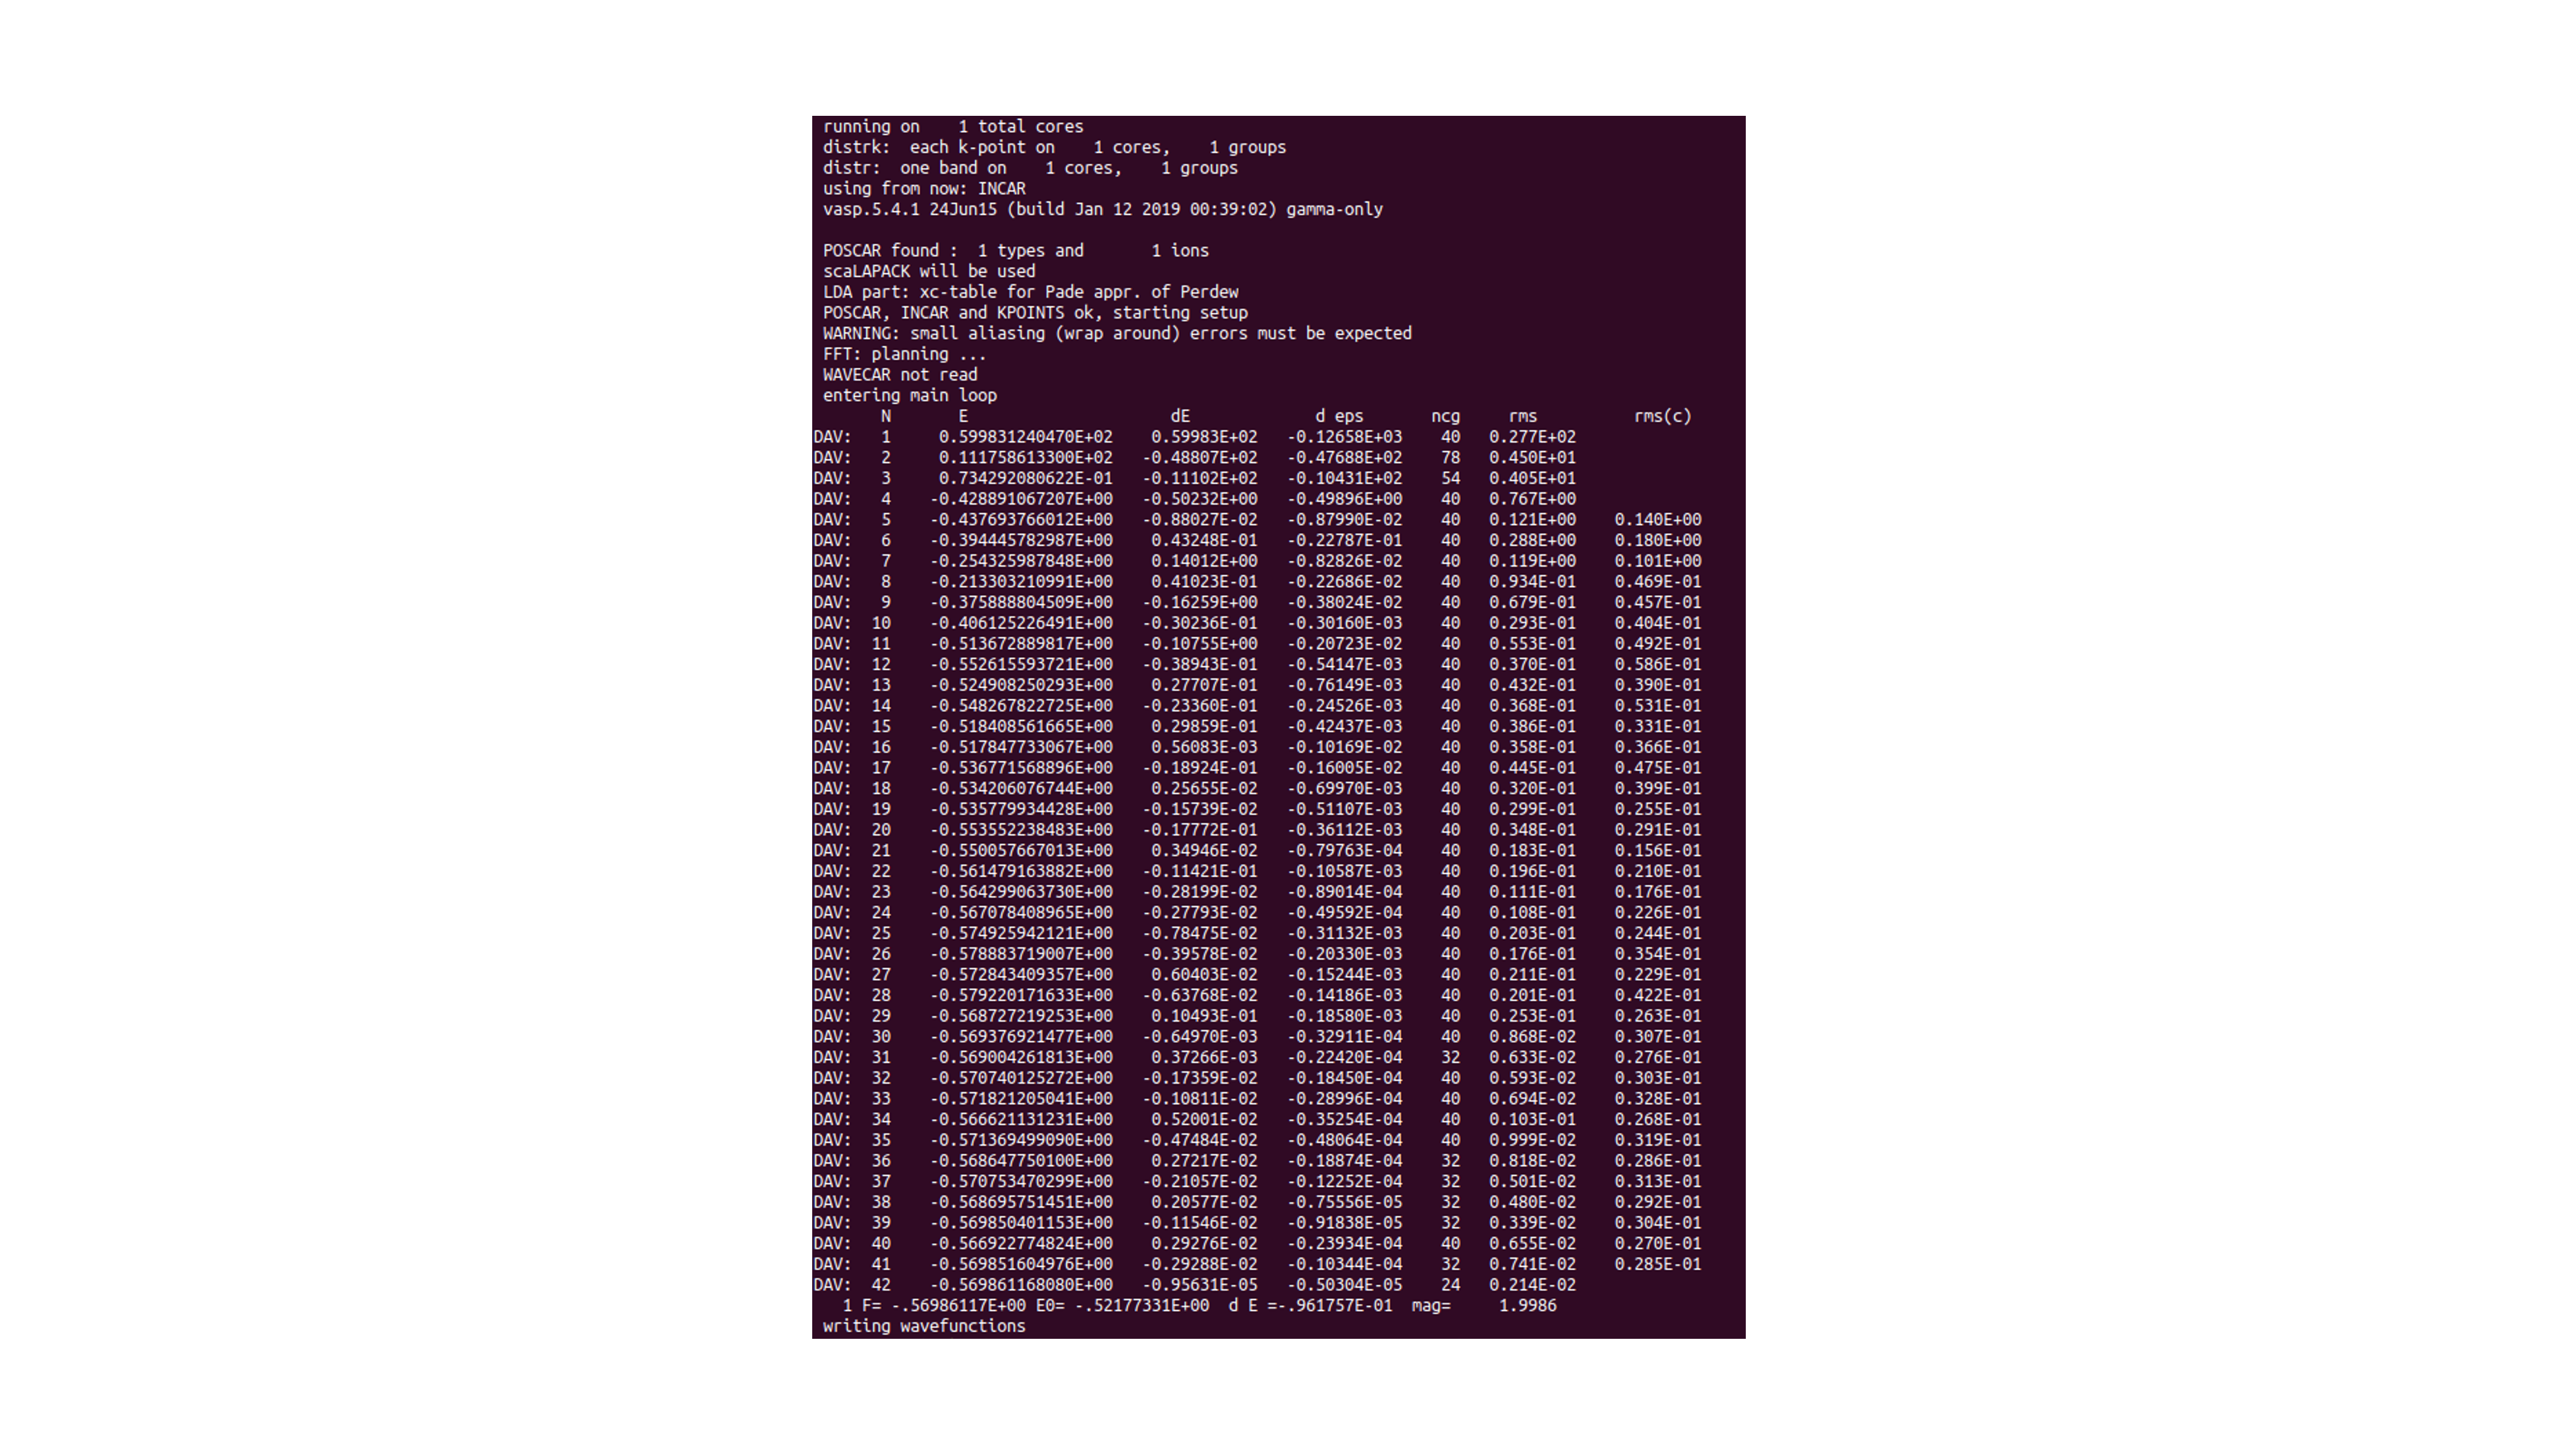
\includegraphics[width=5.9in,viewport=880 0 1870 1465,clip]{Pt_atom-runout.png}
%\caption{\small \textrm{VASP}运行时的屏幕输出.}%(与文献\cite{EPJB33-47_2003}图1对比)
%\label{Pt_atom:runout}
%\end{figure}
%从输出内容中可以看到警告提示\textrm{wrap around},只要是\textrm{VASP}软件认为用于\textrm{FFT}计算的网格不够密,就会出现该提示。该提示提示用户,由于\textrm{FFT}网格不够密集,会导致电荷密度在\textrm{FFT}处理时存在混叠误差\textrm{(aliasing error)}。如果想避免出现该提示,可以搜索输出文件\textrm{OUTCAR}中的参数\textit{NGX/NGY/NGZ}避免混叠误差的推荐值,并在\textrm{INCAR}文件中设定该参数。不过通常情况下此处警告提示可以忽略,因为混叠误差对结果的影响微乎其微。当看到最后一行输出\textrm{writing wavefunctions},就表明\textrm{VASP}正常结束。
%\newpage
%\subsection{\rm{VASP}的结果}
\frame
{
	\frametitle{输出文件}
正常结束的\textrm{VASP}计算,会产生13个输出文件%,见图\ref{Pt_atom:lsout}。
\begin{figure}[h!]
\centering
\vskip -2pt
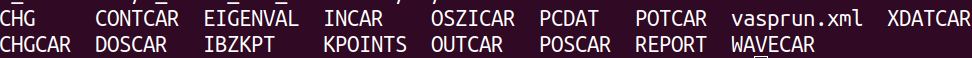
\includegraphics[height=0.20in,width=4.0in,viewport=0 2 750 38,clip]{Figures/Pt_atom-lsout.png}
\caption{\fontsize{6.2pt}{5.2pt}\selectfont{\textrm{VASP}运行结束后的文件.}}%(与文献\cite{EPJB33-47_2003}图1对比)
\label{Pt_atom:lsout}
\end{figure}

%以下先介绍\textrm{OSZICAR}和\textrm{OUTCAR}这两个文件。
%\subsubsection{\rm{OSZICAR}}
{\fontsize{7.5pt}{5.2pt}\selectfont{\textrm{OSZICAR}文件存储的是\textrm{VASP}迭代循环过程中的能量变化情况}}%,部分内容如图\ref{Pt_atom:OSZICAR}所示。
\begin{figure}[h!]
\centering
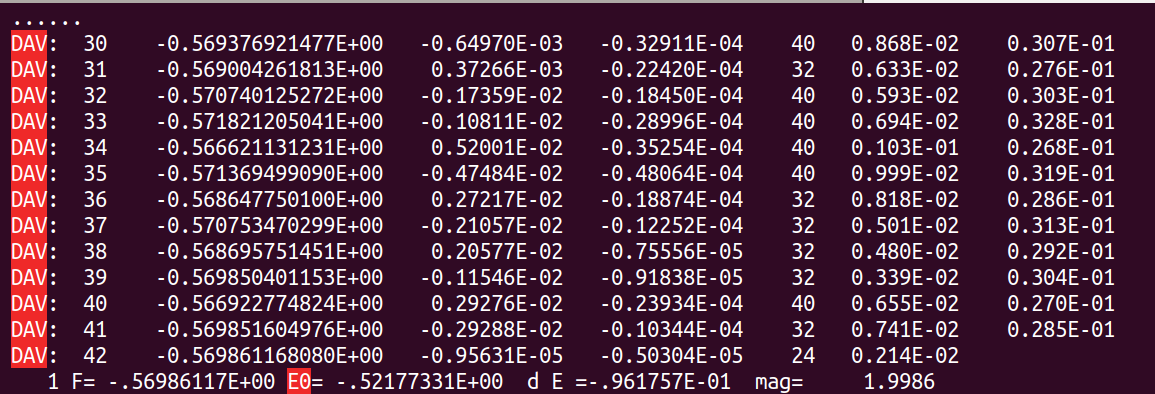
\includegraphics[height=1.2in,width=4.0in,viewport=0 0 880 290,clip]{Figures/Pt_atom-OSZICAR.png}
\caption{\fontsize{6.2pt}{5.2pt}\selectfont{\textrm{VASP}的输出文件\textrm{OSZICAR}(部分).}}%(与文献\cite{EPJB33-47_2003}图1对比)
\label{Pt_atom:OSZICAR}
\end{figure}
}

\frame
{
	\frametitle{\textrm{OSZICAR}}
	各列参数的含义
\begin{itemize}
	\item 第一列~~~:~表示矩阵迭代化的方法
	\item 第二列\textrm{N}:~统计两个离子步计算间的电子步迭代次数
	\item 第三列\textrm{E}:~当前的基态总能
	\item 第三列\textrm{dE}:~两次电子步迭代之间的基态总能变化
	\item 第四列\textrm{d~eps}:~两次电子步迭代的能量本征值的改变%(势保持不变)
	\item 第五列\textrm{ncg}:~完成一次迭代时,\textrm{Hamiltonian}算符\textbf{H}作用于轨道的次数~
	\item 第六列\textrm{rms}:~每次迭代开始时全部占据轨道的初始残矢\textrm{(residual vector)}——$\mathbf{R}=(\mathbf{H}-\varepsilon)\mathbf{S}|\phi\rangle$——之和\\{\fontsize{7.0pt}{5.2pt}\selectfont{该值表明轨道的收敛情形的优劣}}
	\item 第七列\textrm{rms(c)}:~一次迭代前后的电荷密度差
\end{itemize}
}

\frame
{
	\frametitle{\textrm{OSZICAR}}
%\textrm{OSZICAR}的第一列表示计算采用\textrm{Davidson}迭代收敛方法\\第二列为迭代次数%,本算例达到默认的收敛条件($\delta\mathrm{E}<1.0\times10^{-4}~\mathrm{eV}$)共迭代了42次。需要指出的是,
\textrm{Pt}的原子构型为([\textrm{Xe}]$4\mathit{f}^{14}5\mathit{d}^96\mathit{s}^1$)
\vskip 5pt
最后一行$\mathrm{E}_0$的值($-0.522\mathrm{eV}$)就是当前参数设置下,单个\textrm{Pt}原子在真空中的基态能量
{\fontsize{8.5pt}{5.2pt}\selectfont{
\begin{itemize}
	\item $\mathrm{E}_0$不是原子的绝对能量,而是\textrm{Pt}原子相对于\textrm{PAW}势的能量
\end{itemize}}}	
$\mathrm{mag}$的值($1.9986\mu_{\mathrm{B}}$)表示自旋极化计算的原子磁矩%(\textrm{Bohr magneton})
{\fontsize{8.5pt}{5.2pt}\selectfont{
\begin{itemize}
	\item 磁矩来自原子中两个未成对电子:
\begin{displaymath}
	\mathrm{mag}=\mu_{\mathrm{B}}[\rho_{\uparrow}-\rho_{\downarrow}]
\end{displaymath}
\end{itemize}}}
}
%\subsubsection{\rm{OUTCAR}}
\frame
{
	\frametitle{\textrm{OUTCAR}}
	\textcolor{red}{
\textbf{OUTCAR文件是\textrm{VASP}运行过程中最重要的输出文件}%,
}
%\textrm{OUTCAR}保存的是\textrm{VASP}运行中最详尽的过程记录:~

{\fontsize{7.5pt}{5.2pt}\selectfont{文件不仅包括输入文件的既有信息,还有计算体系的对称性分析,$\vec k$空间布点和具体位置,平面波基信息和最近邻原子的距离等基本信息;~此外记录了每一步离子弛豫和电子弛豫的计算信息}}%所以

\textrm{OUTCAR}的文件结构为:~
\begin{itemize}
	\item \textrm{VASP}版本和基本计算环境和计算资源信息
	\item 读入\textrm{INCAR}、\textrm{POTCAR}、\textrm{POSCAR}
	\item 最近邻原子和对称性分析信息
	\item 关于计算过程的详尽的控制参数信息(含默认值)
	\item 晶格正空间和$\vec k$-空间信息与原子坐标
	\item 平面波基信息(截断能和平面波数目)
	\item 非局域赝势信息
	\item 每个电子步计算的信息
	\end{itemize}
}

\frame
{
	\frametitle{\textrm{OUTCAR}}
	\begin{itemize}
		\item 每个电子步迭代的时间和能量信息
	\end{itemize}
\begin{figure}[h!]
\centering
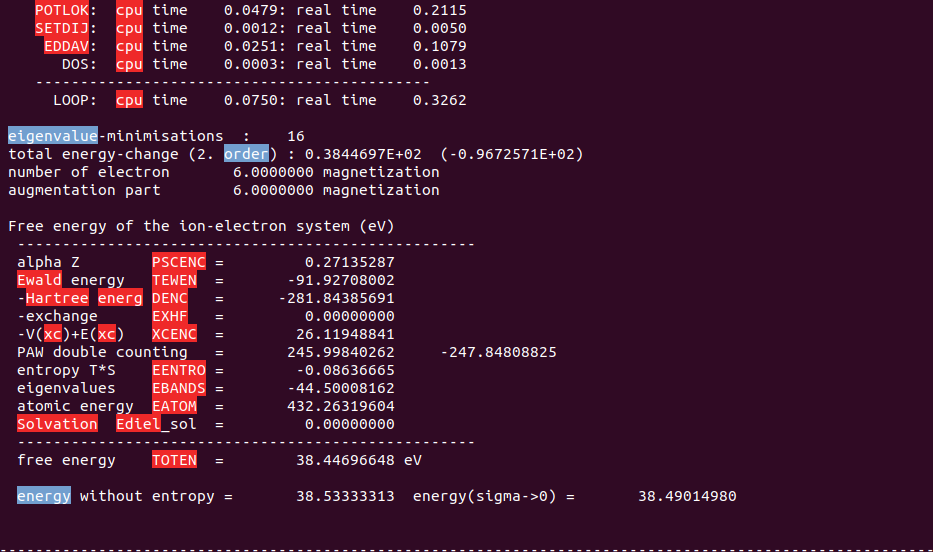
\includegraphics[height=2.5in,viewport=0 40 770 555,clip]{Figures/VASP_train-OUTCAR-iteration.png}
\caption{\fontsize{6.2pt}{5.2pt}\selectfont{\textrm{VASP}的输出文件\textrm{OUTCAR}的电子步迭代信息示例.}}%(与文献\cite{EPJB33-47_2003}图1对比)
\label{VASP_train-OUTCAR-iteration}
\end{figure} 
}

\frame
{
	\frametitle{\textrm{OUTCAR}}
	\begin{itemize}
	\item 能量本征值信息
	\end{itemize}
\begin{figure}[h!]
\centering
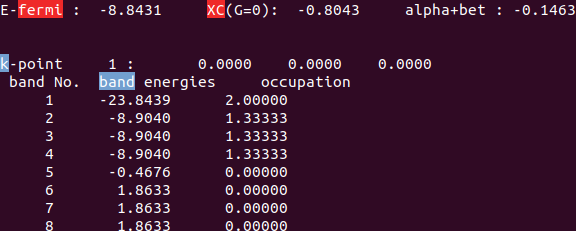
\includegraphics[height=1.5in,viewport=0 0 580 235,clip]{Figures/VASP_train-OUTCAR-eigenvalue.png}
\caption{\fontsize{6.2pt}{5.2pt}\selectfont{\textrm{VASP}的输出文件\textrm{OUTCAR}电子步迭代完成能量本征值信息示例.}}%(与文献\cite{EPJB33-47_2003}图1对比)
\label{VASP_train-OUTCAR-eigenvalue}
\end{figure}
}

\frame
{
	\frametitle{\textrm{OUTCAR}}
	\begin{itemize}
	\item 原子的受力与应力张量和晶胞信息
	\end{itemize}
\begin{figure}[h!]
\centering
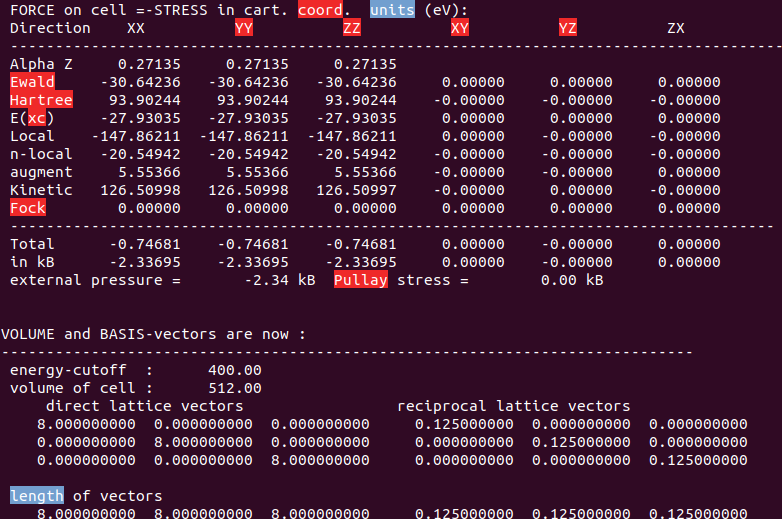
\includegraphics[height=2.5in,viewport=0 0 780 515,clip]{Figures/VASP_train-OUTCAR-stress_and_volumn.png}
\caption{\fontsize{6.2pt}{5.2pt}\selectfont{\textrm{VASP}的输出文件\textrm{OUTCAR}原子受力与应力张量和晶胞信息示例.}}%(与文献\cite{EPJB33-47_2003}图1对比)
\label{VASP_train-OUTCAR-stress_and_volumn}
\end{figure}
}

\frame
{
	\frametitle{\textrm{OUTCAR}}
	\begin{itemize}
	\item 体系基态总能和自由能信息
	\end{itemize}
\begin{figure}[h!]
\centering
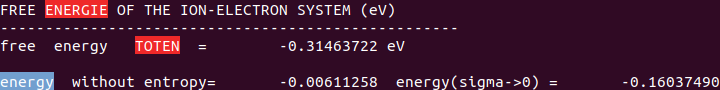
\includegraphics[height=0.5in,viewport=0 0 720 95,clip]{Figures/VASP_train-OUTCAR-free_energy.png}
\caption{\fontsize{6.2pt}{5.2pt}\selectfont{\textrm{VASP}的输出文件\textrm{OUTCAR}基态总能和自由能信息.}}%(与文献\cite{EPJB33-47_2003}图1对比)
\label{VASP_train-OUTCAR-free_energy}
\end{figure}
%}
%
%\frame
%{
%	\frametitle{\textrm{OUTCAR}}
%	\begin{itemize}
%	\item 完整计算过程的资源和计算时间统计信息
%\end{itemize}
%\begin{figure}[h!]
%\centering
%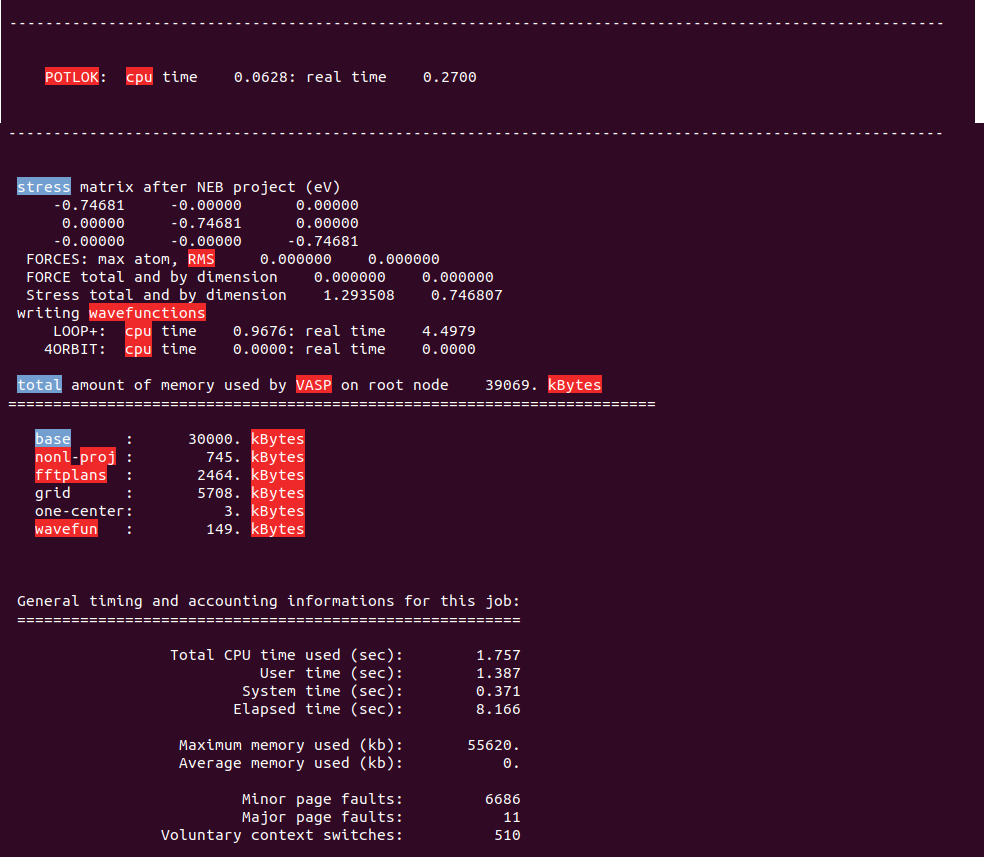
\includegraphics[height=2.7in,width=4.0in,viewport=5 0 680 835,clip]{VASP_train-OUTCAR-time_and_memory.png}
%\caption{\fontsize{6.2pt}{5.2pt}\selectfont{\textrm{VASP}的输出文件\textrm{OUTCAR}的计算资源和时间统计信息.}}%(与文献\cite{EPJB33-47_2003}图1对比)
%\label{VASP_train-OUTCAR-time_and_memory}
%\end{figure}
%}
% 在本算例中,
文件末尾记录的全部计算过程运行时间和计算资源使用情况%,如图\ref{Pt_atom:runtime}所示:
\begin{figure}[h!]
\centering
\vskip -2pt
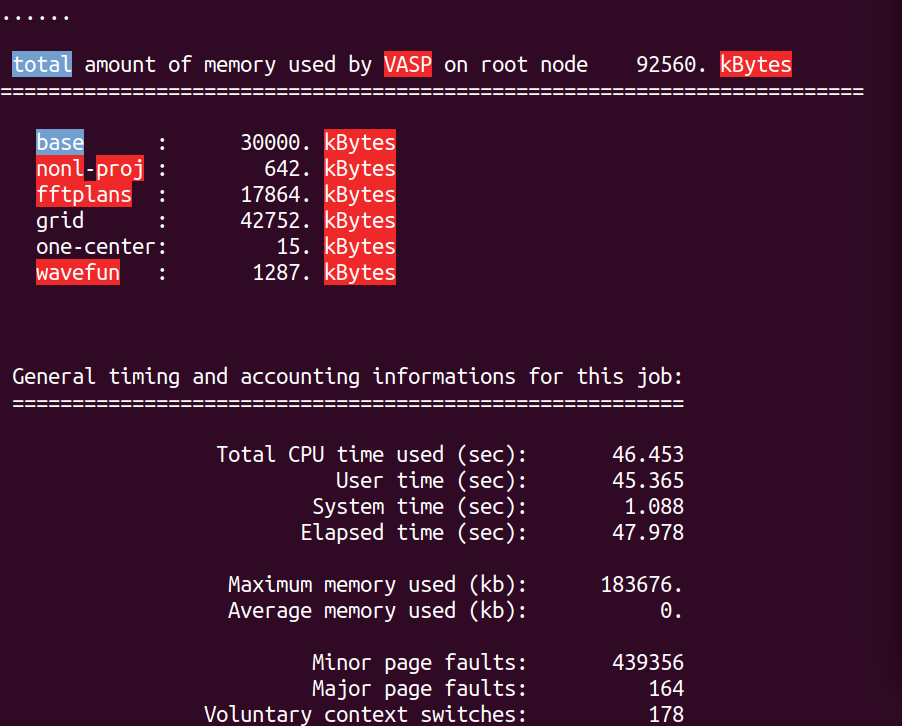
\includegraphics[height=1.2in,width=4.0in,viewport=0 0 680 215,clip]{Figures/Pt_atom-runtime.png}
\caption{\fontsize{6.2pt}{5.2pt}\selectfont{\textrm{VASP}的输出文件\textrm{OUTCAR}最后部分.}}%(与文献\cite{EPJB33-47_2003}图1对比)
\label{Pt_atom:runtime}
\end{figure}
%结果表明,\textrm{VASP}计算简单原子,只需要几十秒即可完成
}

\frame
{
	\frametitle{其余数据文件}
	除\textrm{OSZICAR}和\textrm{OUTCAR}外,还有三个重要的输出文件:~
	\begin{itemize}
		\item \textcolor{blue}{\textrm{CHGCAR}}:~存储体系的电荷密度
		\item \textcolor{blue}{\textrm{CONTCAR}}:~存储体系经结构弛豫后得到的原子位置和晶胞参数
		\item \textcolor{blue}{\textrm{WAVECAR}}:~存储体系最终的波函数文件(非格式输出的二进制文件)
	\end{itemize}
}

%\subsubsection{断点续算}
\frame
{
	\frametitle{断点续算}
\textrm{VASP}计算因故结束后,可以从中断计算位置继续完成计算,从而节约计算时间

执行断点续算的时候,除了需要将\textrm{CONTCAR}的内容复制到\textrm{POSCAR}中,还要对\textrm{INCAR}文件作必要的修改并增添如下内容:
\begin{figure}[h!]
\centering
\vskip -5pt
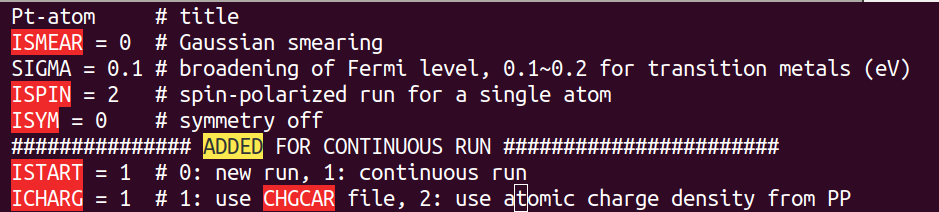
\includegraphics[height=1.0in,width=4.0in,viewport=0 0 700 157,clip]{Figures/Pt_atom-continurun.png}
\caption{\fontsize{6.2pt}{5.2pt}\selectfont{\textrm{VASP}断点续算的输入控制文件\textrm{INCAR}.}}%(与文献\cite{EPJB33-47_2003}图1对比)
\label{Pt_atom:continuruntime}
\end{figure}
再次运行\textrm{VASP},程序除了读取原来四个输入文件的内容,还将读取\textrm{CHGCAR}和\textrm{WAVECAR}的内容%,经过约近二十次迭代后,计算结果将进一步优化$\mathrm{E}_0=-.555\mathrm{~eV/atom}$,磁矩为$\mathrm{mag}=2.0000\mu_{\mathrm{B}}$,这次得到的原子基态能量将被用于后续体相\textrm{Pt}的结合能\textrm{(Cohesive energy)}计算。
}
\subsection{面心立方{\rm Pt}晶胞计算}\label{Sec:FCC-Pt}
%\subsubsection{\rm{POSCAR}}
\frame
{
	\frametitle{面心立方晶胞的结构}
	面心立方\textrm{(Face-centered Cubic, FCC)}结构的\textrm{Pt}晶体,晶胞参数为$a_0=3.975~\mathrm{\AA}$。每个面心立方中含有4个\textrm{Pt}原子
%面心立方\textrm{Pt}的晶胞中含有4个原子,在\textrm{POSCAR}文件中,四个原子分别置于原点和立方体的三个面心位置%。如图\ref{Pt_FCC:structure}所示。
\begin{figure}[h!]
\centering
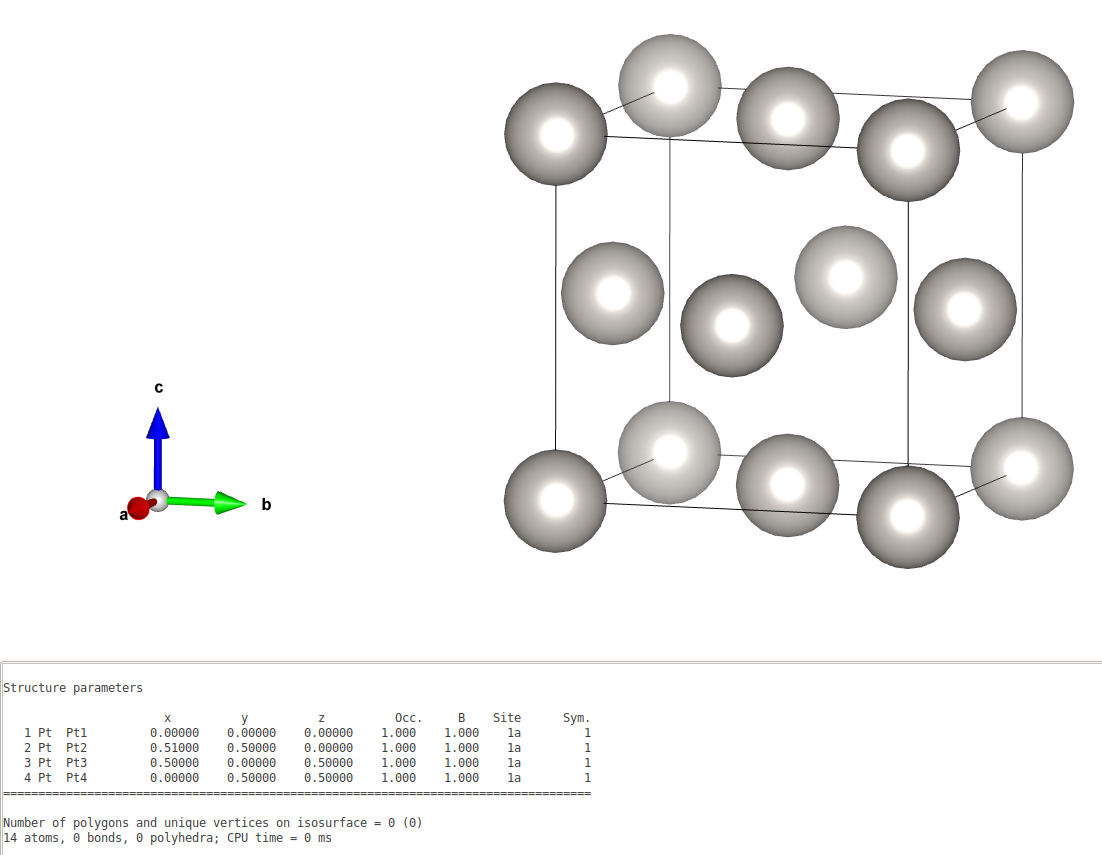
\includegraphics[height=1.8in,viewport=350 210 840 640,clip]{Figures/VASP_train-FCC.png}
\caption{\fontsize{6.2pt}{5.2pt}\selectfont{\textrm{FCC-Pt}的空间结构.}}%(与文献\cite{EPJB33-47_2003}图1对比)
\label{Pt_FCC:structure}
\end{figure}
}

\frame
{
	\frametitle{面心立方晶胞的\textrm{POSCAR}}
\begin{figure}[h!]
\centering
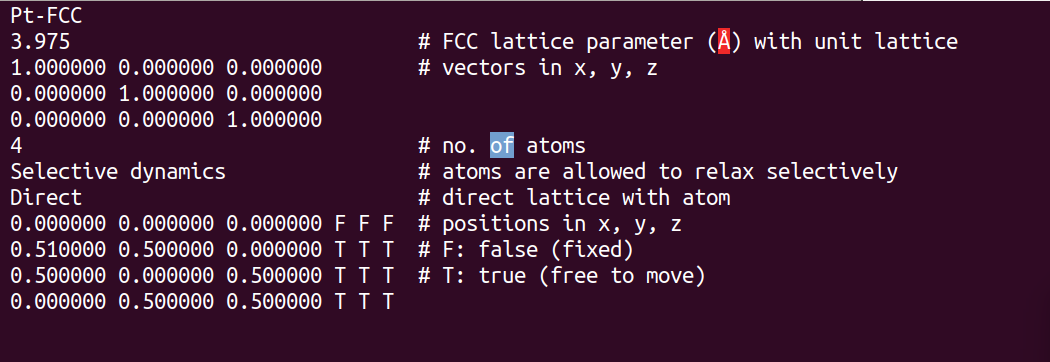
\includegraphics[height=1.3in,width=4.0in,viewport=0 30 740 270,clip]{Figures/Pt_FCC-POSCAR.png}
\caption{\fontsize{6.2pt}{5.2pt}\selectfont{用于\textrm{VASP}计算的\textrm{FCC-Pt}的结构文件\textrm{POSCAR}.}}%(与文献\cite{EPJB33-47_2003}图1对比)
\label{Pt_FCC:POSCAR}
\end{figure}
本算例中,晶胞中第一个\textrm{Pt}原子位置固定,其余三个原子允许在各个维度方向自由移动\\
{\fontsize{7.0pt}{5.2pt}\selectfont{注意到第二个\textrm{Pt}原子在$x$方向上偏移面心立方位置0.01%(见图\ref{Pt_FCC:POSCAR}),
结构弛豫时,如要求保持面心立方对称性,可以预见,经过结构弛豫后,晶胞将回到正常的面心立方位置}}
}

%\subsection{输入文件}
\frame
{
\frametitle{\textrm{INCAR}}
%这里计算的是
%计算\textrm{FCC-Pt},除了\textrm{POTCAR}与\textrm{Pt}原子相同,其余输入原子依次讨论如下:~
%\subsubsection{\rm{INCAR}}
%,计算中不再考虑自旋极化,输入文件\textrm{INCAR}如图\ref{Pt_FCC:INCAR}所示:
\begin{figure}[h!]
\centering
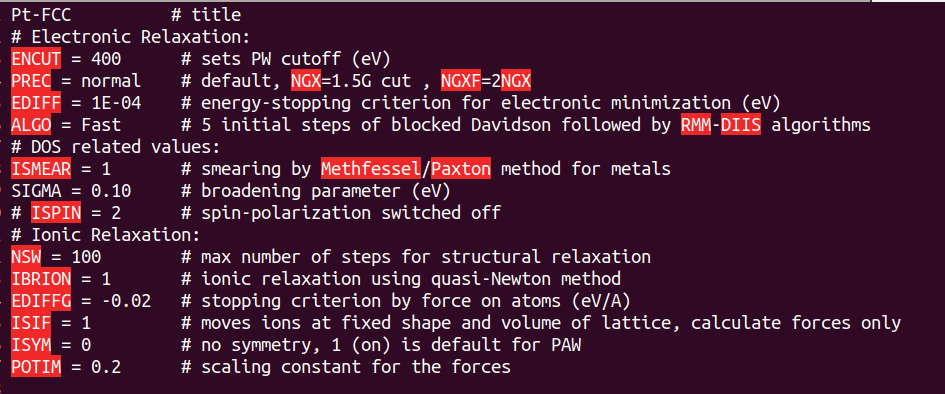
\includegraphics[width=4.0in,viewport=0 0 720 292,clip]{Figures/Pt_FCC-INCAR.png}
\caption{\fontsize{6.2pt}{5.2pt}\selectfont{\textrm{FCC-Pt}的输入控制文件\textrm{INCAR}.}}%(与文献\cite{EPJB33-47_2003}图1对比)
\label{Pt_FCC:INCAR}
\end{figure}
{\fontsize{7.2pt}{5.2pt}\selectfont{对含有偶数个相同原子的晶格,自旋电子密度趋于相同,忽略自旋部分贡献}}
}
%\begin{itemize}
%	\item \textit{ENCUT}:~该参数在需要手工指定平面波\textrm{(Plane Wave, PW)}基组截断能时使用,一旦该参数被指定,由参数\textit{PREC}确定的截断能不再有效。这里\textit{ENCUT}~=~400\textrm{~eV},远高于\textrm{POTCAR}中推荐的能量截断值(\textit{ENMAX}~=~230.283\textrm{~eV}),这样做主要是考虑到后续模拟\textrm{Pt}表面吸附\textrm{O}时,\textit{ENMAX}为400\textrm{~eV},计算组分体系时,平面波截断能应选为不低于最高的\textit{ENMAX}之值。
%	\item \textit{PREC}:~一旦人工指定\textit{ENCUT},参数\textit{PREC}确定的是波函数和电荷密度的\textrm{FFT}变换的网格精度,因此\textit{PREC}也是影响计算精度的参数。绝大多数情况下,参数值\textrm{``normal''}的精度足以满足要求;~如果有更高的精度要求,可以设为\textit{PREC}=\textrm{Accurate}。
%	\item \textit{EDIFF}:~该参数确定的是电子步迭代收敛的截断值,\textrm{VASP}计算中,要求最近邻两个电子步的总能(自由能)和\textrm{Kohn-Sham}方程能量本征值都满足收敛标准,程序才会停止运行。因此对一般计算来说,收敛标准的默认值$1.0\times10^{-4}$,已是足够的高精度。
%	\item \textit{ALGO}:~该参数确定的是离子步嵌套的电子步矩阵迭代对角化算法,参数值\textrm{``fast''}是最常用的,要求除了在第一个离子步弛豫时,最初五个电子步迭代采用稳定的\textrm{Davidson}算法,后续电子步迭代采用\textrm{RMM-DIIS}算法;~其余离子步弛豫,则只有第一个电子步弛豫采用\textrm{Davidson}算法,其余电子步都采用\textrm{RMM-DIIS}算法。
%	\item \textit{EDIFFG}:~该参数确定的是离子步弛豫的收敛截断值。当截断值为正,则要求最近邻两个离子步的总能(自由能)满足收敛标准;~当截断值为负,则要求计算对象中的每个原子上的受力都小于该值的绝对值(因此是更严格的收敛标准),默认值为$0.02\mathrm{eV/\AA}$。在没有达到收敛标准之前,程序将不断移动原子的位置;~在达到收敛标准之后,将不再改变体系中原子的位移。
%\end{itemize}
%对于一个新的\textrm{VASP}计算任务,初始波函数(也称为初猜波函数)可以通过原子赝势构造,这是符合物理直觉的。从不同截断能或不同结构的计算态出发,无疑将会节省计算时间。其余参数留待后续计算中说明。当需要对比两个体系的总能时,要确保两个体系的精度参数要求相同,这些参数包括:~\textit{ENCUT}、\textit{PREC}、\textit{EDIFF}、\textit{EDIFFG}和\textit{ISMEAR}。
%\subsubsection{\rm{KPOINTS}}
\frame
{
	\frametitle{\textrm{KPOINTS}}
$\vec k$空间布点数为$9\times9\times9$,布点方案由\textrm{Monkhorst-Pack}方法生成,这是对于金属和导体非常适用的布点方法%。如图\ref{Pt_FCC:KPOINTS}所示。
\begin{figure}[h!]
\centering
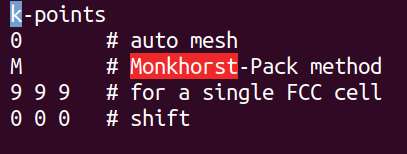
\includegraphics[width=4.0in,viewport=0 0 330 118,clip]{Figures/Pt_FCC-KPOINTS.png}
\caption{\fontsize{6.2pt}{5.2pt}\selectfont{\textrm{VASP}计算\textrm{FCC-Pt}的输入文件\textrm{KPOINTS}.}}%(与文献\cite{EPJB33-47_2003}图1对比)
\label{Pt_FCC:KPOINTS}
\end{figure}
}
%\subsection{用shell脚本运行VASP计算}
%\subsubsection{脚本运行}
%这里学习用\textrm{shell}脚本来提交\textrm{VASP}运行任务,后面的练习也将用脚本提交任务。提交\textrm{VASP}计算的\textrm{shell}脚本(文件名为\textcolor{green}{\textrm{run.vasp}})的内容如图\ref{Pt_FCC:run}所示:
%\begin{figure}[h!]
%\centering
%\vskip -12pt
%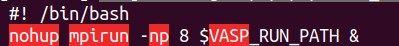
\includegraphics[height=0.3in,viewport=0 0 380 45,clip]{Pt_FCC-run.png}
%\caption{\small 提交\textrm{VASP}计算任务\textrm{FCC-Pt}的\textrm{shell}脚本内容.}%(与文献\cite{EPJB33-47_2003}图1对比)
%\label{Pt_FCC:run}
%\end{figure}
%	\begin{itemize}
%		\item 命令形式\textcolor{magenta}{~\textrm{nohup}~[执行命令]~\&~}表示将执行命令提交为后台进程,这样即使当前用户在计算执行过程中执行别的计算命令甚至退出,也不会影响计算任务正常的执行。这里\textrm{``nohup''}是\textrm{``no hang-up''}的缩写。
%		\item 命令中\textcolor{magenta}{\textrm{mpirun~-np~8~}}表示此次\textrm{VASP}计算用8个\textrm{CPU}并行完成。
%		\item \textcolor{magenta}{\$\textrm{VASP\_RUN\_PATH~}}表示\textrm{VASP}的执行文件的路径。
%	\end{itemize}
%将该执行脚本和\textrm{VASP}计算的四个输入文件放在同一个目录下,加可执行权限:~\\
%\textcolor{magenta}{chmod~+x~run.vasp}\\% \# change the file mode to execution mode\\
%然后就可以运行如下命令执行\textrm{VASP}计算:\\
%	\textcolor{magenta}{./run.vasp }\\
%		计算过程中,通过\textrm{Hellman-Feynman}定理计算作用在每个离子步位置上的原子受力,离子步迭代过程直到全部原子的受力都满足收敛标准\textit{EDIFFG}($0.02\mathrm{eV/\AA}$)。在计算过程中,可以通过以下命令监控原子受力情况的变化:\\
%		\textcolor{magenta}{grep~\`~drift~\'~ OUTCAR}
%\subsubsection{\rm{nohup.out}}
%用\textcolor{magenta}{$\mathrm{nohup}~[\cdots]~\&$}提交的任务,计算过程会保存在输出文件\textrm{nohup.out}中,如图\ref{Pt_FCC:nohupout}所示。
%%\newpage
%\begin{figure}[h!]
%\centering
%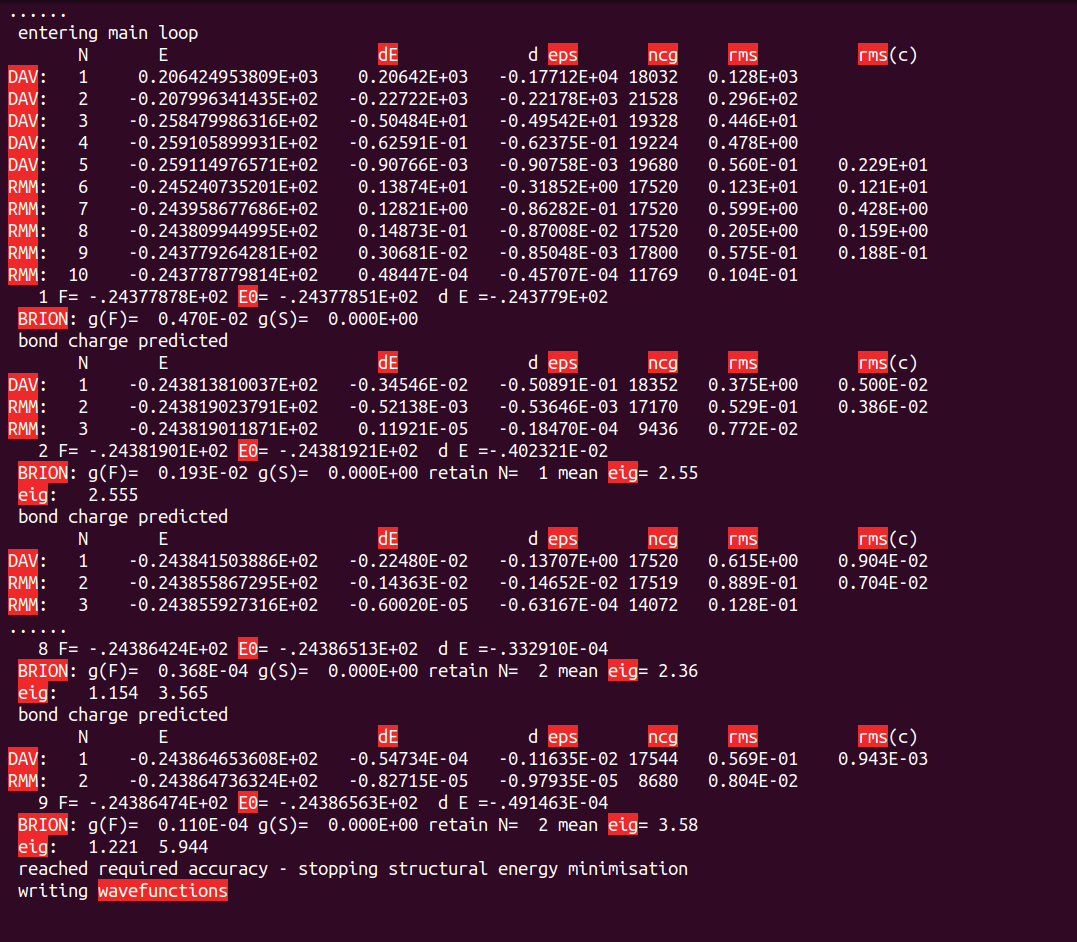
\includegraphics[height=5.5in,viewport=0 20 620 730,clip]{Pt_FCC-nohupout.png}
%\caption{\small \textrm{VASP}计算\textrm{FCC-Pt}的输出文件\textrm{nohup.out}.}%(与文献\cite{EPJB33-47_2003}图1对比)
%\label{Pt_FCC:nohupout}
%\end{figure}
%
%因为参数\textit{ALGO}=\textrm{fast},因此第一次离子步弛豫中,最初5步电子步迭代的矩阵对角化是\textrm{Davidson}方法,然后是\textrm{RMM-DIIS}方法;~电子步迭代结束后,根据原子受力,将原子移动到新的位置(完成离子弛豫),在新的原子构型下开始电子步迭代,循环往复,直到满足收敛标准(\textit{EDIFF}和\textit{EDIFFG})。最后出现的\textrm{``writing wave functions''}表明运行结束。波函数将写入\textrm{WAVECAR}文件中(参照\textrm{INCAR}中的输出设置)。
%\subsection{计算结果}
%\subsubsection{\rm{CONTCAR}与结构弛豫}
\frame
{
	\frametitle{结构弛豫:~\textrm{CONCAR}}
\textrm{CONTCAR}文件记录的是结构弛豫完成时晶体中原子的位置%,本算例\textrm{FCC-Pt}弛豫后的\textrm{CONTCAR}内容如图\ref{Pt_FCC:CONTCAR}所示。
\begin{figure}[h!]
\centering
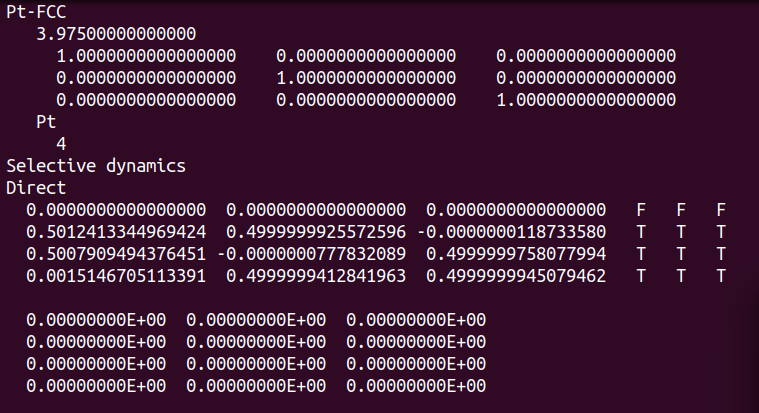
\includegraphics[width=4.0in,viewport=0 0 580 230,clip]{Figures/Pt_FCC-CONTCAR.png}
\caption{\fontsize{6.2pt}{5.2pt}\selectfont{\textrm{VASP}计算中记录\textrm{FCC-Pt}弛豫后结构的文件\textrm{CONTCAR}.}}%(与文献\cite{EPJB33-47_2003}图1对比)
\label{Pt_FCC:CONTCAR}
\end{figure}
{\fontsize{7.0pt}{5.2pt}\selectfont{显然,结构弛豫后,第二个原子由起始位置\textrm{(0.510000,~0.500000,~0.00000)}弛豫到\textrm{FCC}结构要求的原子位置(存在一定的数值误差)}}
}
\frame
{
	\frametitle{从\textrm{OUTCAR}中提取信息}
%\subsubsection{\rm{OUTCAR}}
%为监控
	离子步弛豫过程中体系总能量收敛情况%,可以使用以下命令检索输出文件\textrm{OUTCAR}:\\
%\textcolor{magenta}{\textrm{grep~~\'~energy~without~entropy~\'~~OUTCAR}}\\
%结果如图\ref{Pt_FCC:OUTCAR_totene}所示。
\begin{figure}[h!]
\centering
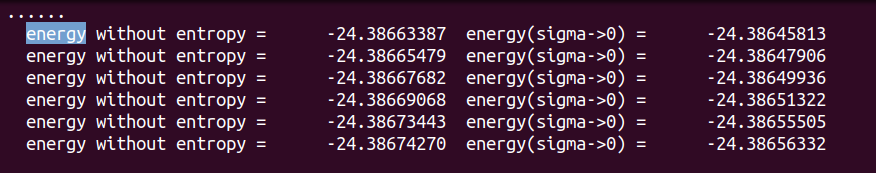
\includegraphics[width=4.0in,viewport=0 0 680 130,clip]{Figures/Pt_FCC-OUTCAR_totene.png}
\caption{\fontsize{6.2pt}{5.2pt}\selectfont{\textrm{VASP}计算\textrm{FCC-Pt}的弛豫过程的基态总能收敛情况.}}%(与文献\cite{EPJB33-47_2003}图1对比)
\label{Pt_FCC:OUTCAR_totene}
\end{figure}
{\fontsize{7.2pt}{5.2pt}\selectfont{离子步迭代收敛时的基态能量$\mathrm{E}_0$的值为~$-24.387\mathrm{~eV}$,换言之,当面心立方的晶胞参数为$3.975\mathrm{\AA}$时,体系中\textrm{Pt}原子的基态能量为$-24.387/4=-6.097\mathrm{eV/atom}$,比%\ref{Sec:atom-Pt}节计算的
孤立原子\textrm{Pt}的基态能量要低}}
}
%下一节我们将讨论晶胞参数的优化和影响\textrm{VASP}计算精度的重要参数的确定。
\subsection{收敛测试}\label{Sec:convergence}
\frame
{
	\frametitle{能量收敛测试}
对\textrm{DFT}迭代计算过程,随着迭代次数递增,体系总能(或自由能)会快速下降,随后进到逐渐平稳变化的区域,并伴随小的振荡,最终达到基态能量,%如图\ref{Fig:convergence}所示,
这个过程称为\textbf{收敛}。
\begin{figure}[h!]
	\vskip -5pt
\centering
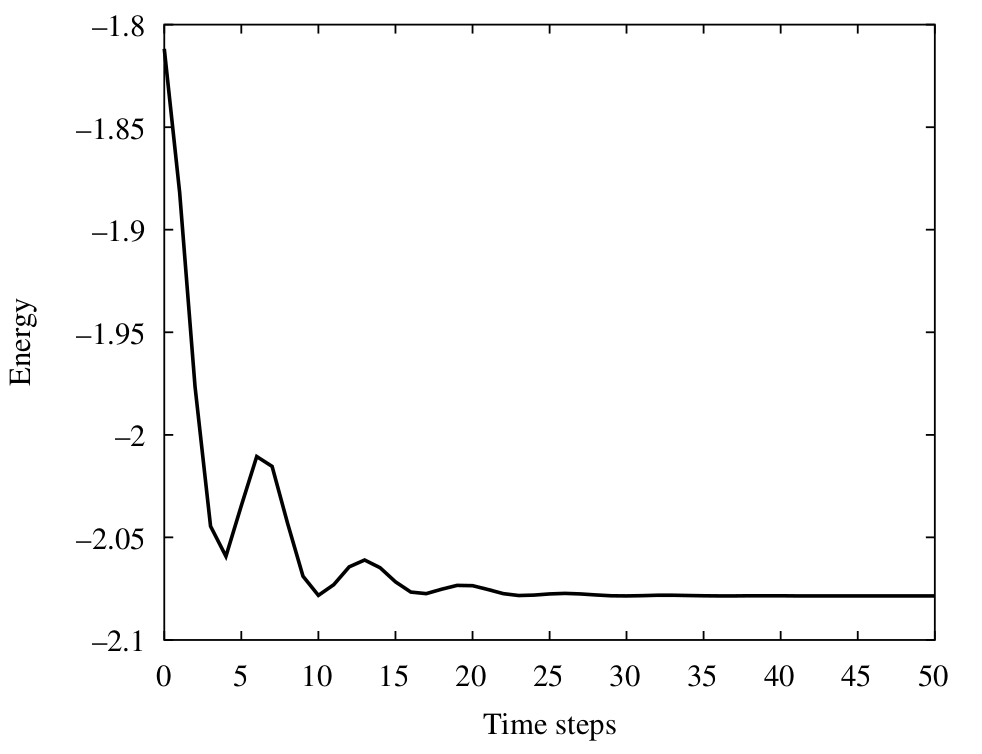
\includegraphics[width=3.0in,viewport=0 33 740 600,clip]{Figures/Ab-initio-Ene.png}
\caption{\fontsize{6.2pt}{5.2pt}\selectfont{迭代计算中的能量收敛示意图,引自文献\cite{Comp_Phys}.}}%(与文献\cite{EPJB33-47_2003}图1对比)
\label{Fig:convergence}
\end{figure}
{\fontsize{7.0pt}{5.2pt}\selectfont{对于任何研究体系,首先必须保证迭代计算能收敛,然后才谈得上进行有意义的\textrm{DFT}计算。同时,面对一个全新的计算体系,合理的收敛测试也是非常必要的,否则难免遭遇为克服迭代计算收敛的困难,浪费过多计算资源和精力}}
}

%考虑到\textrm{DFT}计算的本质是变分过程,因此只有各种初始条件选择都比较合理,计算才可能收敛到正确的结果,否则很可能收敛到错误的结果。在收敛测试中,最重要的参数主要包括:
%\begin{itemize}
%	\item \textrm{INCAR}中的参数\textit{ENCUT}
%	\item \textrm{KPOINTS}中的$\vec k$空间布点数目
%\end{itemize}
%在正常收敛测试中,两个参数的数值都应该由小到大逐渐增加,这将有助于考察计算体系的总能是否随参数逐渐趋于收敛。
%\subsection{能量收敛测试}
%体系截断能的定义
%\begin{equation}
%	E_{\mathrm{cut}}\geqslant\dfrac12|\vec k+\vec G|^2
%	\label{eq:Ecut}
%\end{equation}
%换句话说,截断能确定的是平面波基波矢的上限。一般截断能的取值范围是$150\sim400\mathrm{~eV}$,其默认阈值由计算体系组成元素的\textrm{POTCAR}中\textit{ENMAX}和\textit{ENMIN}中的极大值和极小值确定。但是,在具体计算过程中,合理的截断能应该通过测试确定。本次练习使用的\textrm{shell}脚本中,将包含3个输入文件(\textrm{INCAR},\textrm{KPOINTS}和\textrm{POSCAR})的设置,并且有4个不同的截断能参数\textit{ENCUT}(200,~225,~250和350\textrm{~eV})。计算中$\vec k$空间布点数固定($9\times9\times9$)。由此可以同时确定\textit{ENCUT}的收敛情况和平衡态晶胞参数。
%\subsubsection{\rm{shell}脚本\rm{run.lattice}}
%这里给出一个\textrm{shell}脚本的范例(文件名\textcolor{green}{\textrm{run.lattice}}),如图\ref{Pt_FCC-runlattice}所示,当前截断能为\textit{ENCUT}=250\textrm{~eV}。
%\begin{figure}[h!]
%\centering
%\hspace*{-20pt}
%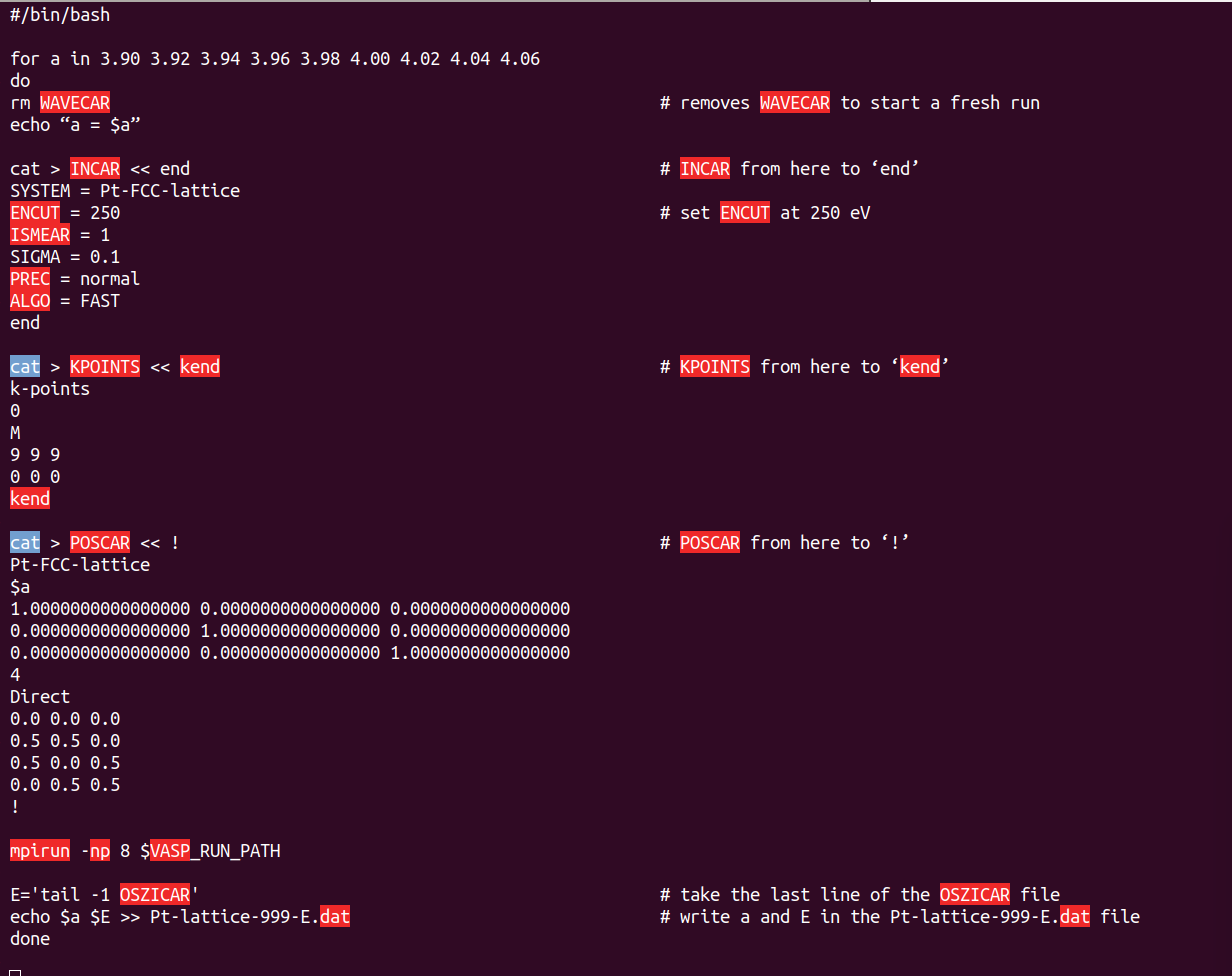
\includegraphics[height=5.2in,viewport=0 20 860 700,clip]{Pt_FCC-OUTCAR_runlattice.png}
%\caption{\small \textrm{FCC-Pt}截断能收敛测试\textrm{shell}脚本\textrm{run.lattice}示例.}%(与文献\cite{EPJB33-47_2003}图1对比)
%\label{Pt_FCC-runlattice}
%\end{figure}
%
%从该\textrm{shell}脚本内容看,晶胞参数将\textrm{\$a}从$3.90\mathrm{\AA}$到$4.06\mathrm{\AA}$变化,并且每改变一次晶胞参数将会执行一轮\textrm{VASP}晶格弛豫计算流程。因为是收敛测试,而平面波的收敛与自旋无关,因此\textrm{VASP}计算不考虑自旋极化的影响。
%
%有必要指出的是,在\textrm{shell}脚本中,生成\textrm{INCAR}、\textrm{KPOINTS}和\textrm{POSCAR}文件的各命令行必须连续,不能被注释或空行隔断,这一点请初学者务必注意。
%\subsubsection{\rm{测试脚本的执行}}
%与\ref{Sec:FCC-Pt}的\textrm{shell}脚本执行类似,首先可执行权限:\\
%\textcolor{magenta}{\textrm{
%chmod~+x~./run.lattice}}\\% \# change the file mode to execution mode\\
%再运行:\\
%\textcolor{magenta}{\textrm{./run.lattice }}
%\subsubsection{\rm{执行结果}}
%脚本执行完毕,结果将写入到文件\textrm{Pt-lattice-999-E.dat}中。因此当截断能\textit{ENCUT}=250\textrm{~eV}时,\textrm{FCC-Pt}的不同晶胞参数下得到不同的基态总能,可用命令\\
%\textcolor{magenta}{\textrm{cat~Pt-lattice-999-E.dat}}\\
%查看,如图\ref{Pt_FCC-energy-con}所示。
%\begin{figure}[h!]
%\centering
%\vskip -8pt
%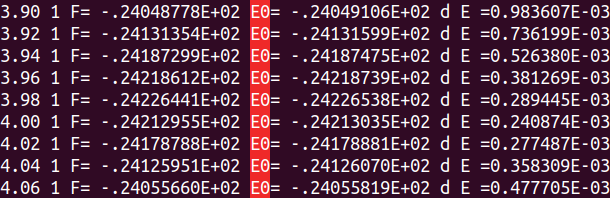
\includegraphics[height=1.3in,viewport=0 0 620 200,clip]{Pt_FCC-energy-con.png}
%\caption{\small \textrm{FCC-Pt}截断能收敛测试:~不同晶胞参数下的基态总能.}%(与文献\cite{EPJB33-47_2003}图1对比)
%\label{Pt_FCC-energy-con}
%\end{figure}
%
%图\ref{Pt_FCC-energy-curve}给出的是
%四种不同的截断能(分别是200,~225,~250和350\textrm{~eV})下的运行结果,截断能在\textit{ENCUT}=250\textrm{~eV}时,总能达到收敛(差别小于5\textrm{~meV})。平衡态的晶格参数为$3.077\mathrm{\AA}$,该值与\textrm{Bentmann}等的计算值$3.975\mathrm{\AA}$\cite{PRB78-205302_2008}吻合得很好,与实验值$3.928\mathrm{\AA}$\cite{Kittel}也较为接近。根据优化参数得到的体系总能为~--24.2269\textrm{~eV}(--6.057\textrm{~eV/atom})。
\frame
{
	\frametitle{截断能收敛测试}
\begin{figure}[h!]
\centering
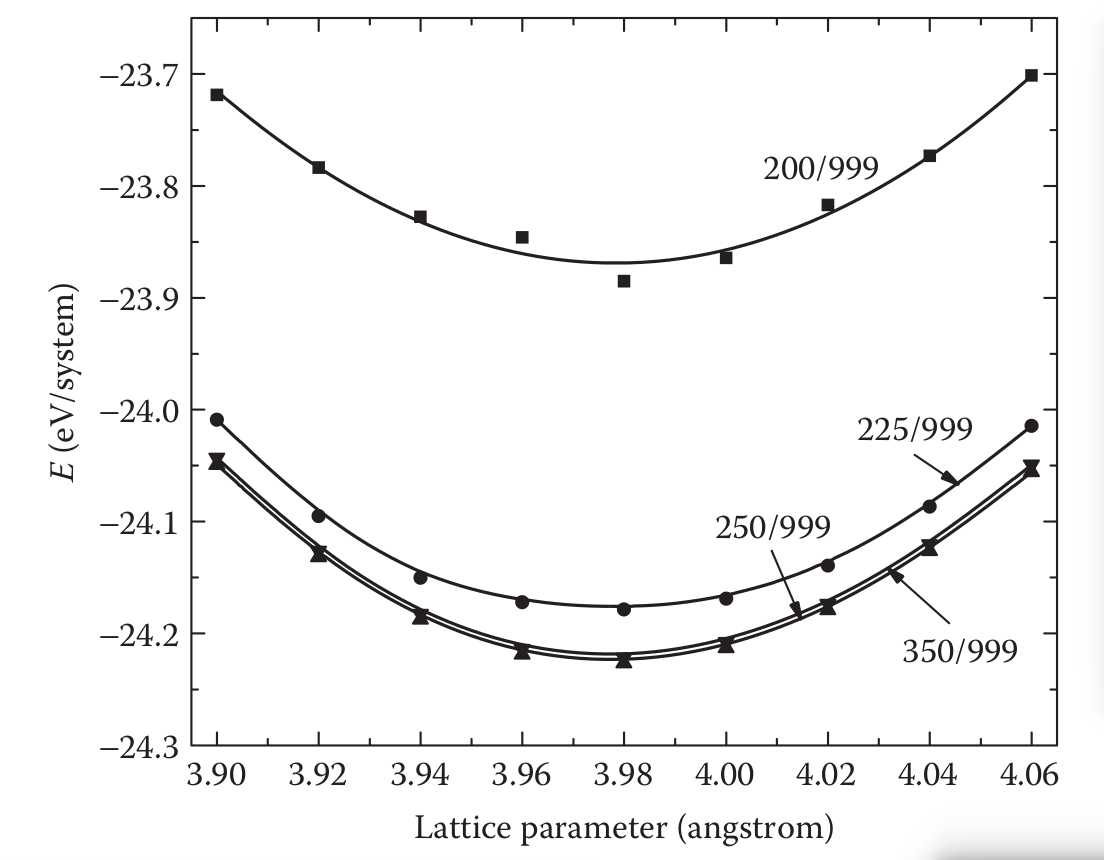
\includegraphics[width=2.8in,viewport=0 11 820 650,clip]{Figures/Pt_FCC-Ecut-convergence.png}
\caption{\fontsize{6.2pt}{5.2pt}\selectfont{\textrm{FCC-Pt}截断能收敛测试:~不同截断能下的基态总能曲线($\vec k$-点数目$9\times9\times9$).}}%(与文献\cite{EPJB33-47_2003}图1对比)
\label{Pt_FCC-energy-curve}
\end{figure}
{\fontsize{7.2pt}{5.2pt}\selectfont{不难预见,随着截断能的增加,计算时长将会增加($\vec k$点增加的情形类似)}}
}
%。关于\textit{ENCUT}的设置注意以下事项:
%\begin{itemize}
%	\item 对于多元素组分的体系,一般默认最高的截断能作为体系截断能;
%	\item 对于需要比照的体系,计算时应将\textit{ENCUT}和\textrm{KPOINTS}的数值设置成相同;
%	\item 对于晶格形状和体积都可以弛豫(\textit{ISIF}=3)的体系,一般\textit{ENCUT}比默认值增大$\sim30\%$,并设置参数\textit{PREC}=\textrm{accurate}
%\end{itemize}

%由截断能的定理式\eqref{eq:Ecut}可知,随着\textit{ENCUT}的增大,每个\textrm{k}-点上用于展开轨道的平面波数目的相应变化,将会呈现$\mathrm{N}_{\mathrm{PW}}\propto E_{\mathrm{cut}}^{3/2}$的基本规律。这一点可以在\textrm{OUTCAR}中查找平面波数目得到印证。命令为:~\\
%\textcolor{magenta}{\textrm{grep~\`~plane waves\`~OUTCAR}}\\
%图\ref{Pt_FCC-PW}给出当截断能\textit{ENCUT}=250\textrm{~eV}时,部分$\vec k$点上用于展开波函数的平面波基组的数目。
%\begin{figure}[h!]
%\centering
%\vskip -8pt
%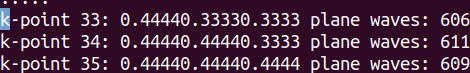
\includegraphics[height=0.6in,viewport=0 0 500 80,clip]{Pt_FCC-PW.png}
%\caption{\small \textrm{FCC-Pt}截断能收敛测试:~截断能为250\textrm{~eV}时各$\vec k$点的平面波基数目(部分).}%(与文献\cite{EPJB33-47_2003}图1对比)
%\label{Pt_FCC-PW}
%\end{figure}
%
%此外,在\textrm{OUTCAR}中,\textit{NPLWV}表示\textrm{FFT}变换的总的网格点数($\mathit{NGX}\times\mathit{NGY}\times\mathit{NGZ}$),这里$\mathit{NGX}$, $\mathit{NGY}$和$\mathit{NGZ}$分别对应$x$-,$y$-和$z$-方向的网格点数。如果对比不同晶体结构的\textrm{Pt}体系,如六方密堆积的\textrm{HCP-Pt}和体心立方的\textrm{BCC-Pt}完成相同的结构弛豫,我们将会发现,面心立方结构\textrm{FCC-Pt}具有最低的基态能量,亦即具有是最稳定的基态结构。这部分内容作为课后练习,留给大家自行完成并验证上述结论。

%\subsection{$\vec k$点收敛测试}
\frame
{
	\frametitle{$\vec k$点收敛测试}
一旦确定合适的\textrm{ENCUT},可用类似的方式确定$\vec k$点数目%。利用晶体对称性,倒空间中的均匀网格点将被约化到不可约\textrm{Brillouin}区(\textrm{Irreducible Brillouin Zone,~IBZ})中。这些不可约$\vec k$-点作为$\vec k$空间的积分权重点,将会用于体系物性计算。当确定参数\textit{ENCUT}为250\textrm{~eV},平衡态晶格常数为$3.977\mathrm{\AA}$后,依次增加$\vec k$-空间网格布点(由$2\times2\times2$到$10\times10\times10$),直至总能的能量差是收敛到$\sim1\mathrm{meV}$。
%
%输出文件\textrm{IBZKPT}中保存的是\textrm{IBZ}区域的$\vec k$点信息,随着$\vec k$点数的增加,\textrm{IBZ}的网格点将由1增大到35。
\begin{figure}[h!]
\centering
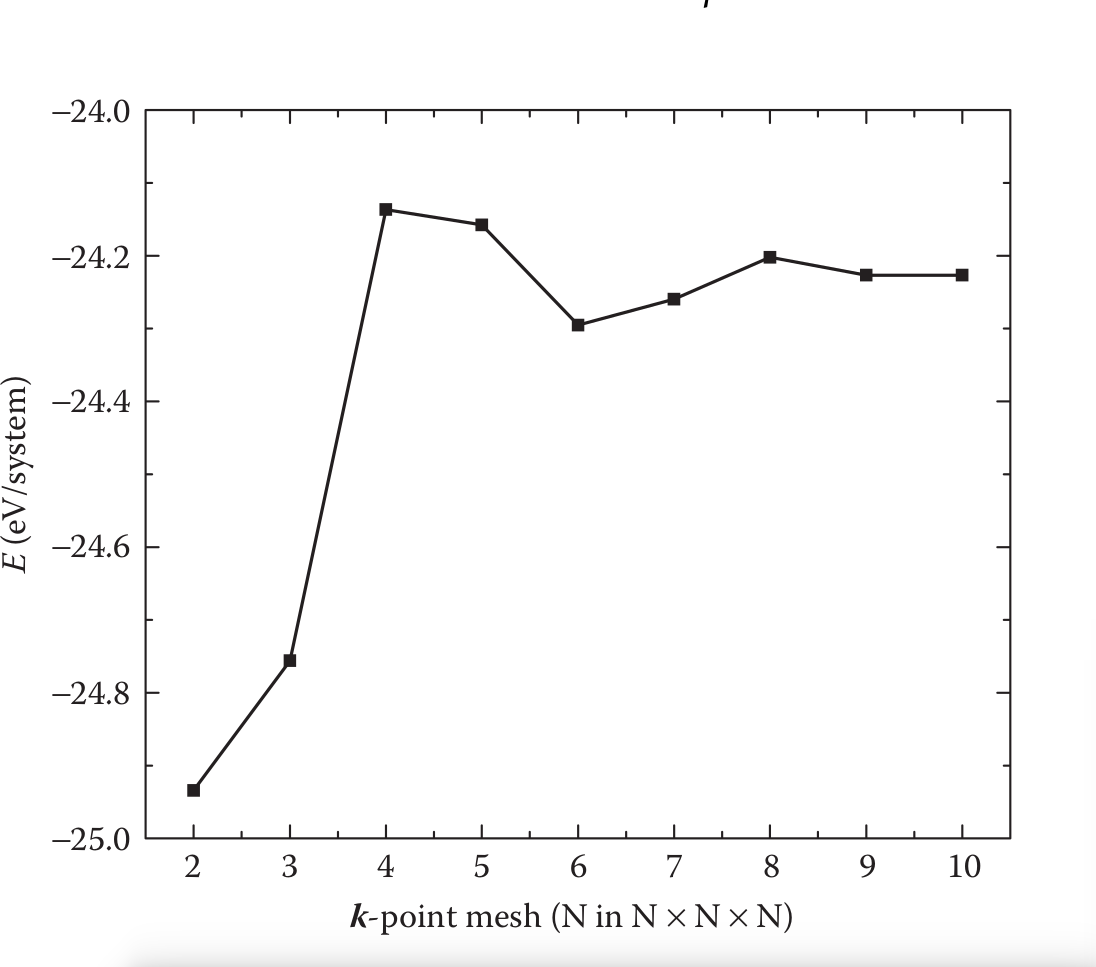
\includegraphics[width=2.8in,viewport=0 11 820 650,clip]{Figures/Pt_FCC-kpoint-convergence.png}
\caption{\fontsize{6.2pt}{5.2pt}\selectfont{\textrm{FCC-Pt}截断能收敛测试:~基态总能随$\vec k$-点变化的曲线(截断能\textrm{ENCUT}=250\textrm{~eV}).}}%(与文献\cite{EPJB33-47_2003}图1对比)
\label{Pt_FCC-kpoint-curve}
\end{figure}
{\fontsize{6.2pt}{5.2pt}\selectfont{$\vec k$-点收敛测试与\textit{ENCUT}收敛的情形类似}}%,结果如图\ref{Pt_FCC-kpoint-curve}所示。从图中不难看出,对于当前体系,$9\times9\times9$的网格点能保证足够精度。
%需要指出的是,从文件\textrm{IBZKPT}中的$\vec k$点分布看,采用\textrm{Monkhorst-Pack}布点方案,将每个维度格点剖分成偶数时,$\vec k$空间的网格点分布会更均匀。
}
\subsection{{\rm Pt}超晶胞计算}\label{Sec:bulk-Pt}
%下面我们将学习由32个\textrm{Pt}原子构成的超晶胞(\textrm{FCC}晶胞按$2\times2\times2$堆积得到)的基本的物理性质计算:~重点掌握内聚能\textrm{(cohesive energy)}和空位形成能\textrm{(vavanvy formation energy)}的计算。为简明起见,前面介绍过的参数,今后不再作详细说明。
%\subsection{Pt超晶胞的内聚能计算}
\frame
{
	\frametitle{\textrm{Pt}超晶胞内聚能计算:~输入文件}
%为了计算内聚能,首先计算理想超晶胞的\textrm{Pt}基态能量。输入控制文件\textrm{INCAR}的修改部分如图\ref{Pt_Bulk-INCAR-modified}所示:~
	{\fontsize{7.4pt}{5.2pt}\selectfont{计算中不再要求输出电荷密度和波函数到\textrm{CHGCAR}和\textrm{WAVECAR},设置控制参数\textcolor{blue}{\textit{ISYM}}=1}}
\begin{figure}[h!]
\centering
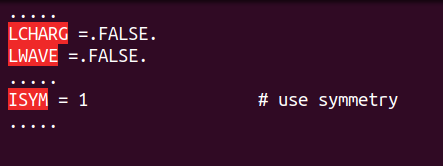
\includegraphics[height=0.8in,viewport=0 20 340 118,clip]{Figures/Pt_Bulk-INCAR.png}
%\includegraphics[height=1.8in,width=4.in,viewport=30 210 570 440,clip]{PAW_projector.eps}
\caption{\fontsize{6.2pt}{5.2pt}\selectfont{\textrm{计算\textrm{Pt}超晶胞时\textrm{INCAR}文件的修改部分.}}}%(与文献\cite{EPJB33-47_2003}图1对比)
\label{Pt_Bulk-INCAR-modified-1}
\end{figure}
\begin{figure}[h!]
\centering
\vskip -3pt
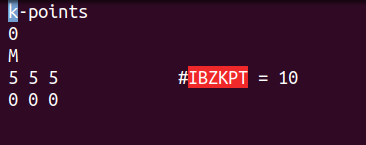
\includegraphics[height=0.8in,viewport=0 20 240 108,clip]{Figures/Pt_Bulk-KPOINTS.png}
%\includegraphics[height=1.8in,width=4.in,viewport=30 210 570 440,clip]{PAW_projector.eps}
\caption{\fontsize{6.2pt}{5.2pt}\selectfont{\textrm{计算\textrm{Pt}超晶胞时的\textrm{KPOINTS}文件.}}}%(与文献\cite{EPJB33-47_2003}图1对比)
\label{Pt_Bulk-KPOINTS}
\end{figure}
{\fontsize{6.2pt}{5.2pt}\selectfont{超晶胞是由8倍的\textrm{FCC-Pt}构成,$\vec k$-点数约简为$5\times5\times5$}}%,\textrm{KPOINTS}文件如图\ref{Pt_Bulk-KPOINTS}所示:~
}

\frame
{
	\frametitle{\textrm{Pt}超晶胞内聚能计算:~输入文件}
%考虑到\ref{Sec:FCC-Pt}已经得到\textrm{FCC-Pt}结构弛豫后的晶胞,因此$2\times2\times2$堆积的超晶胞中原子起始结构如图\ref{Pt_Bulk-POSCAR}所示。虽然\textrm{INCAR}中的控制参数允许晶胞结构弛豫,超晶胞的\textrm{POSCAR}文件中的原子也仍保持可移动状态,但可以预见,体系的弛豫计算不应该带来很显著的形变。
\begin{figure}[h!]
\centering
\vskip -5pt
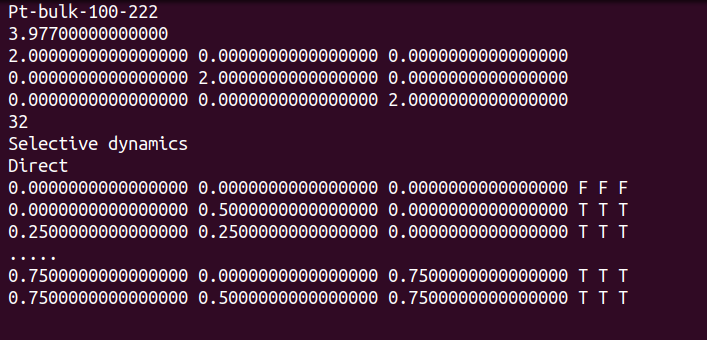
\includegraphics[height=2.0in,viewport=0 25 500 270,clip]{Figures/Pt_Bulk-POSCAR.png}
%\includegraphics[height=1.8in,width=4.in,viewport=30 210 570 440,clip]{PAW_projector.eps}
\caption{\fontsize{6.2pt}{5.2pt}\selectfont{\textrm{计算\textrm{Pt}超晶胞时的\textrm{POSCAR}文件(部分).}}}%(与文献\cite{EPJB33-47_2003}图1对比)
\label{Pt_Bulk-POSCAR}
\end{figure}
}

\frame
{
	\frametitle{\textrm{Pt}超晶胞内聚能计算:~运算输出}
%用\ref{Sec:FCC-Pt}的\textrm{shell}脚本\textcolor{green}{\textrm{run.vasp}}提交计算任务至后台运行,计算过程中可以检查输出文件\textrm{nohup.out}或\textrm{OSZICAR}的内容可以监控计算过程,图\ref{Pt_Bulk-OSZICAR}给出\textrm{nohup.out}的部分结果:
\begin{figure}[h!]
\centering
\hspace*{-5pt}
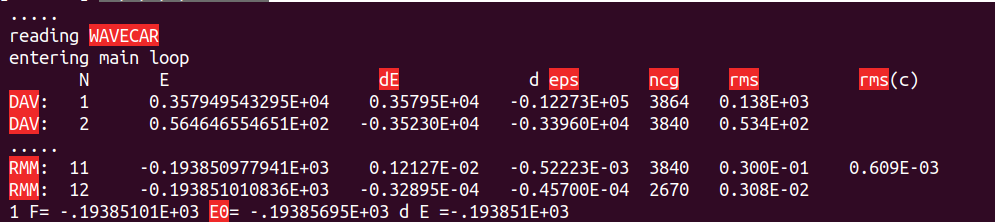
\includegraphics[width=4.0in,viewport=0 0 950 215,clip]{Figures/Pt_Bulk-OSZICAR.png}
%\includegraphics[height=1.8in,width=4.in,viewport=30 210 570 440,clip]{PAW_projector.eps}
\caption{\fontsize{6.2pt}{5.2pt}\selectfont{\textrm{计算\textrm{Pt}超晶胞时的迭代输出\textrm{OSZICAR}文件(局部).}}}%(与文献\cite{EPJB33-47_2003}图1对比)
\label{Pt_Bulk-OSZICAR}
\end{figure}
{\fontsize{7.2pt}{5.2pt}\selectfont{\textrm{VASP}程序为快速收敛,设定完成前五次电子步迭代后,才开始电荷密度的迭代,所以最初\textrm{5}次电子步迭代时,没有\textrm{rms(c)}输出%。电子步结束时,最后一行的\textrm{F}表示电子步达到收敛的自由能,

根据同一行的$\mathrm{E}_0$值(0\textrm{K}时$\sigma\rightarrow0$),可以算出超晶胞中的单个原子\textrm{Pt}的能量为$-193.8569/32=-6.058\mathrm{~eV/atom}$

不难看出,该值比晶格参数为$3.975\mathrm{\AA}$时计算的\textrm{FCC-Pt}的原子能量$-6.056\mathrm{eV/atom}$仅有微小变化}}
}
%如果迭代计算过程中出错,\textrm{VASP}将会输出错误或警告提示信息,并终止程序运行。此外也可以通过\textrm{kill}命令终止程序。命令为:~\\
%\textcolor{magenta}{\textrm{killall -9 VASP\_pid}}\\
%这里\textrm{VASP\_pid}是当前执行的\textrm{VASP}进程号。
%
%如果计算过程中发现有参数或设置问题,可以在计算目录中产生一个\textrm{STOPCAR}文件,并向其中增添一行内容:~\\
%\textit{LSTOP}=\textrm{.TRUE.}\\
%则正在运行的\textrm{VASP}程序会在当前离子步结束并输出\textrm{WAVECAR}和\textrm{CHGCAR}后,进入下一离子步计算时退出运行。一般用户可以在修正发现的错误后,在现有计算基础上,继续向下完成整个计算任务。

%\subsubsection{内聚能}
\frame
{
	\frametitle{内聚能计算}
内聚能\textrm{(Cohesive energy) $E_{\mathrm{coh}}$}:~\\
体相的平均原子能量和自由原子能量$E_{\mathrm{atom}}$的能量差
\vskip 3pt
{\fontsize{7.5pt}{5.2pt}\selectfont{内聚能是衡量原子构成固体时原子间相互作用强弱的参数}}%,也是材料的一个基本属性。换句话说,
\vskip 5pt
内聚能可通过固体原子在平衡态附近的极小值扣除自由原子能量得到:%。因此可以用以下两个值计算内聚能:~
\begin{displaymath}
	\begin{aligned}
		E_{\mathrm{bulk}}&=-193.85695/32=-6.058~\mathrm{eV/atom}\\
		E_{\mathrm{coh}}&=E_{\mathrm{atom}}-E_{\mathrm{bulk}}=(-0.528)-(-6.058)=5.53\mathrm{eV/atom}
	\end{aligned}
\end{displaymath}
{\fontsize{7.5pt}{5.2pt}\selectfont{该值与文献记载的计算值5.53\textrm{~eV/atom}\upcite{PRB78-205302_2008}一致,与实验值5.45\textrm{~eV/atom}\upcite{Landolt-Bornstein}的数值吻合}}
}

%\subsection{\rm{Pt}的空位生成能计算}
\frame
{
	\frametitle{\textrm{Pt}的空位生成能计算:~模型设计}
室温条件下,金属体相内空位浓度约为$10^{-6}$量级
\vskip 5pt
{\fontsize{7.5pt}{5.2pt}\selectfont{显然不可能为了模拟一个空位,就用$10^6$量级的超晶胞。合理的做法应该是选择合适尺度的超晶胞并设计原子空位,要求超晶胞间空位相互作用可以忽略,由此计算晶格中的空位能}}%。因为计算的超晶胞中仅有一个空位,计算时将\textrm{INCAR}中关闭对称性。

\textrm{POSCAR}文件%可以从之前的超晶胞算例中\textrm{copy}来,
将总的原子扣除位于(0.5,~0.5,~0.5)处的\textrm{Pt}原子,产生空位%,如图\ref{Pt_vacancy-POSCAR}所示:~
\begin{figure}[h!]
\centering
\vskip -3pt
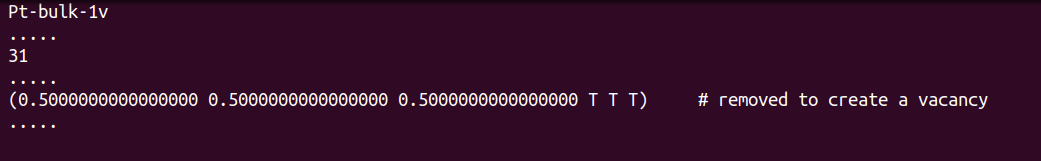
\includegraphics[height=0.85in,viewport=0 15 750 120,clip]{Figures/Pt_vacancy-POSCAR.png}
%\includegraphics[height=1.8in,width=4.in,viewport=30 210 570 440,clip]{PAW_projector.eps}
\caption{\fontsize{6.2pt}{5.2pt}\selectfont{\textrm{模拟\textrm{FCC-Pt}超晶胞中含有一个空位时\textrm{POSCAR}文件的修改部分.}}}%(与文献\cite{EPJB33-47_2003}图1对比)
\label{Pt_vacancy-POSCAR}
\end{figure}
}

\frame
{
	\frametitle{\textrm{Pt}的空位生成能计算}
\begin{figure}[h!]
\centering
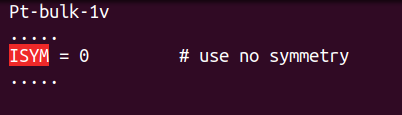
\includegraphics[height=0.9in,viewport=0 15 370 180,clip]{Figures/Pt_vacancy-INCAR.png}
%\includegraphics[height=1.8in,width=4.in,viewport=30 210 570 440,clip]{PAW_projector.eps}
\caption{\fontsize{6.2pt}{5.2pt}\selectfont{\textrm{\textrm{FCC-Pt}超晶胞计算的\textrm{INCAR}文件修改部分.}}}%(与文献\cite{EPJB33-47_2003}图1对比)
\label{Pt_Bulk-INCAR-modified-2}
\end{figure}
与\textrm{Pt}超晶胞计算类似,由\textrm{OSZICAR}文件可知,含有31个\textrm{Pt}原子和一个空位的超晶胞基态能量是$-186.95325\mathrm{~eV/atom}$
}
%\subsubsection{空位形成能}

\frame
{
	\frametitle{\textrm{Pt}的空位生成能计算}
根据空位形成能$E_{\mathrm{v}}^f$的定义可以有:~
\begin{displaymath}
	\begin{aligned}
		E_{\mathrm{v}}^f=&E_{\mathrm{v}}-\dfrac{N-1}N\times E_{\mathrm{bulk}}\\
		=&-186.95325-\dfrac{31}{32}(-193.85695)\\
		=&0.846\mathrm{eV/atom}
	\end{aligned}
\end{displaymath}
{\fontsize{6.2pt}{5.2pt}\selectfont{$E_{\mathrm{v}}$是含有一个空位的超晶胞基态总能,$N$是理想超晶胞的原子个数,$E_{\mathrm{bulk}}$是理想晶体的总能(算例中值是~$-193.85695~\mathrm{eV}$)}}
%我们这里的

计算结果与其他计算值$0.68\mathrm{~eV/vacancy}$或通过正电子子湮灭测量的值$1.35\mathrm{~eV/vacancy}$\upcite{PSSA102-47_1987}有不小的差别\footnote{\fontsize{6.2pt}{5.2pt}\selectfont{\textrm{Mattsson}等发现,只要引入体系的表面误差校正,就能改善\textrm{Pt}的空位形成能,结果为1.18\textrm{eV/vacancy}\upcite{PRB66-214110_2002}。对于其他的材料,比如\textrm{W}\upcite{JNM383-244_2009}或\textrm{SiC}\upcite{JMS44-1828_2009},用\textrm{DFT}计算的缺陷形成能与实验值吻合得比较好}}

由\textrm{CONTCAR}文件中可以看到空位附近原子的弛豫情况%。\textrm{WAVECAR}是二进制文件,保存的是最终得到的电子轨道波函数,亦即\textrm{Kohn-Sham}方程的解。在本次算例中,因为\textrm{INCAR}中的设置,则未将波函数写到\textrm{WAVECAR}中。
}
%\subsubsection{\rm{CHGCAR}绘图}
\frame
{
	\frametitle{\textrm{CHGCAR}图示}
\textrm{VASP}将电荷密度写到\textrm{CHG}和\textrm{CHGCAR}文件,这两个文件的内容基本相同%,主要包括:~晶格矢量、原子位置,电荷密度等。表示电荷密度的网格与超晶胞的形态成正比,网格的数目由\textrm{OUTCAR}中\textrm{FFT}变换的网格数\textit{NFXF}、\textit{NGYF}和\textit{NGZF}确定。将\textrm{CHGCAR}或\textrm{CHG}中的电荷密度按超晶胞体积划分,就可以得到电荷密度的轮廓。例如,本次练习得到的\textrm{CHGCAR}文件的内容如图\ref{Pt_vacancy-CHGCAR}所示:~
\begin{figure}[h!]
\centering
\vskip -5pt
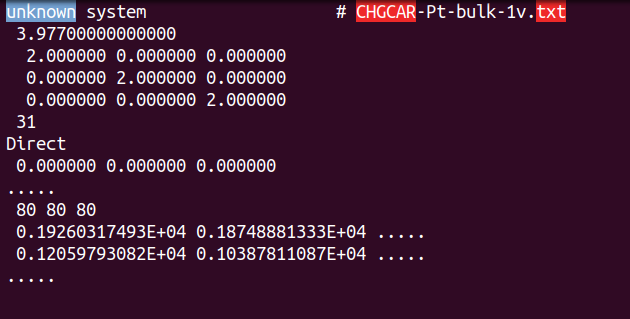
\includegraphics[width=4.0in,viewport=0 20 490 240,clip]{Figures/Pt_vacancy-CONTCAR.png}
%\includegraphics[height=1.8in,width=4.in,viewport=30 210 570 440,clip]{PAW_projector.eps}
\caption{\fontsize{6.2pt}{5.2pt}\selectfont{\textrm{计算\textrm{FCC-Pt}超晶胞出现空位时的\textrm{CHGCAR}文件(部分).}}}%(与文献\cite{EPJB33-47_2003}图1对比)
\label{Pt_vacancy-CHGCAR}
\end{figure}
}

\frame
{
	\frametitle{\textrm{CHGCAR}图示}
	用开源软件如\textcolor{cyan}{\textrm{VASPview}}%\upcite{url_p4vasp}
	或\textcolor{cyan}{\textrm{VESTA}}%\upcite{url_VESTA}
	可将\textrm{CHGCAR}文件的电荷密度可视化%,效果如图\ref{Pt_vacancy-Density}所示:
\begin{figure}[h!]
\centering
\vskip -8pt
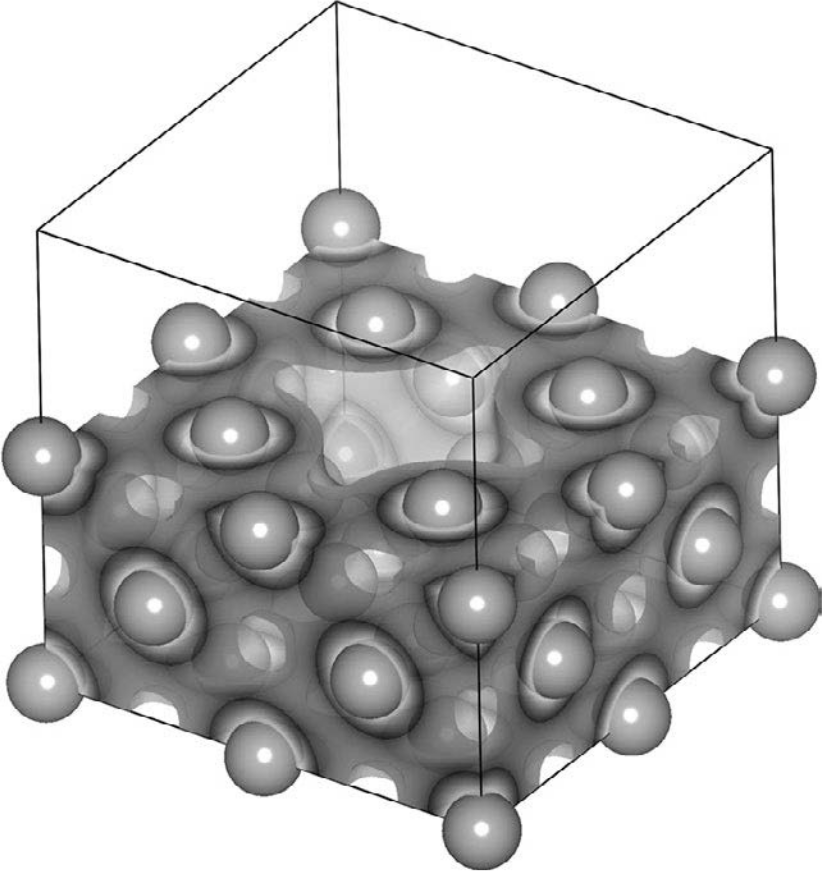
\includegraphics[height=2.0in,viewport=0 0 640 660,clip]{Figures/Pt_vacancy-CHGCAR.png}
%\includegraphics[height=1.8in,width=4.in,viewport=30 210 570 440,clip]{PAW_projector.eps}
\caption{\fontsize{6.2pt}{5.2pt}\selectfont{\textrm{计算\textrm{FCC-Pt}超晶胞出现空位时的图像.}}}%(与文献\cite{EPJB33-47_2003}图1对比)
\label{Pt_vacancy-Density}
\end{figure}
{\vskip -8pt\fontsize{6.8pt}{5.2pt}\selectfont{注意:~图中空位附近的空白区域(图中只显示了超晶胞的下半区域)和每个原子附近近乎均匀分布的电子分布}}
}

\frame
{
	\frametitle{其它超晶胞-缺陷性质计算}

类似地,间隙形成能\textrm{(the formation energies of an interstitial)}$E_{\mathrm{inter}}^f$定义为
\begin{displaymath}
	E_{\mathrm{inter}}^f=E_{\mathrm{inter}}^{\mathrm{bulk}}-E^{\mathrm{bulk}}-nE^{\mathrm{atom}}
\end{displaymath}
{\fontsize{6.2pt}{5.2pt}\selectfont{这里$E_{\mathrm{inter}}^{\mathrm{bulk}}$和$E^{\mathrm{bulk}}$是带有间隙的超晶胞和理想超晶胞的总能,$n$是间隙处的原子数目,$E^{\mathrm{atom}}$是孤立原子的能量}}

进一步推广,如果存在两个固相\textrm{A}和{B},它们可以形成\textrm{AB}相,则三个体相的能量能量差
\begin{displaymath}
	\Delta H_{\mathrm{AB}}=E_{\mathrm{AB}}^{\mathrm{bulk}}-E_{\mathrm{A}}^{\mathrm{bulk}}-E_{\mathrm{B}}^{\mathrm{bulk}}
\end{displaymath}
定义为固体生成焓\textrm{(the formation enthalpy)}
\vskip 5pt
\textcolor{purple}{各种缺陷的形成能都可用简化模型来模拟}\\
{\fontsize{7.0pt}{5.2pt}\selectfont{用户在构造包含缺陷的超晶胞时,必须切记,超晶胞要设计得足够大,确保缺陷间的相互作用足够小}}
}

\subsection{\rm{Pt~(111)}表面的计算}\label{Sec:Surface-Pt}
\frame
{
	\frametitle{材料表面属性}
体相材料的表面有很多基本性质,如
\begin{itemize}
	\item 表面能\textrm{(surface energy)}
	\item 功函数\textrm{(work function)}
	\item 吸附能\textrm{(adsorption energy)}
	\item 吸附原子迁移势垒\textrm{(barrier energy for transport of the adatom)}
\end{itemize}
实际应用中,材料的表面性质具有特殊的重要性%可用来确定材料的用途
{\fontsize{8.0pt}{5.2pt}\selectfont{
	\begin{itemize}
		\item 表面能是表面形貌学研究(向外/向内弛豫、重构、屈服分析)和裂纹扩散到断裂研究的重要因素
		\item 功函数、吸附能/解吸能和势垒能量是研究表面氧化、薄膜表面和纳米结构的生长和稳定、腐蚀、钝化和催化反应的决定因素%。只有真正理解了这些表面现象,才有望从设计层面获得更高性能的材料。本节中,我们将学习构建\textrm{Pt}原子构成的表面,并研究上述提到的表面属性的计算。
	\end{itemize}
}}
}
%\subsection{\rm{Pt~(111)}表面}
\frame
{
	\frametitle{\textrm{Pt~(111)}面\textrm{Slab}:~输入文件}
	{\fontsize{9.5pt}{5.2pt}\selectfont{构建\textrm{Pt~(111)}面\textrm{slab}并计算其基态总能、弛豫能和表面能的计算方案}}%\footnote{\fontsize{6.2pt}{5.2pt}\selectfont{至于选择\textrm{Pt~(111)}面作为研究对象,是因为这个表面在\textrm{Pt}催化材料中研究得最多}}%。这些数据将成为后续进一步计算吸附能和迁移势垒能量的参考基准。
%\subsubsection{\rm{INCAR}}
%\textrm{INCAR}文件的内容如图\ref{Pt_Slab-INCAR}所示:~
\begin{figure}[h!]
\centering
\vskip -5pt
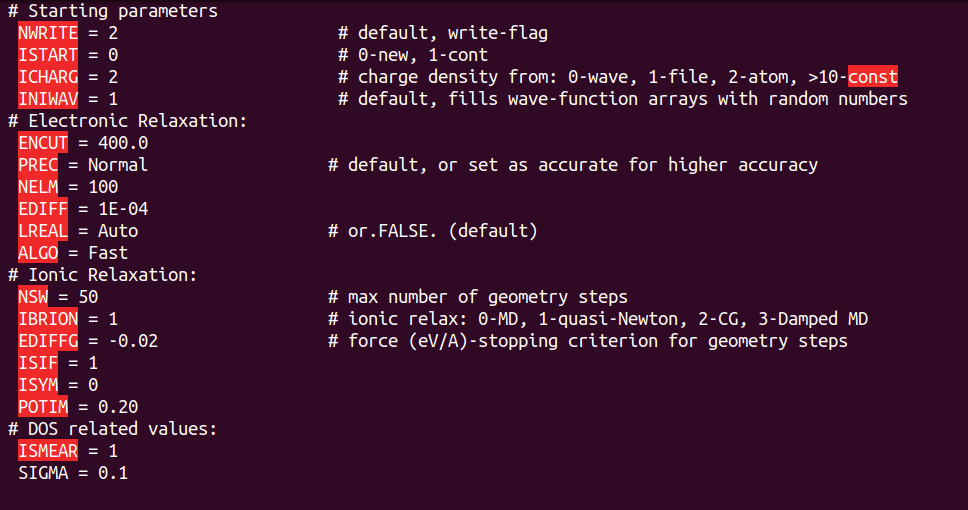
\includegraphics[height=1.5in,viewport=0 10 690 388,clip]{Figures/Pt_Slab-INCAR.png}
%\includegraphics[height=1.8in,width=4.in,viewport=30 210 570 440,clip]{PAW_projector.eps}
\caption{\fontsize{6.2pt}{5.2pt}\selectfont{\textrm{计算\textrm{Pt}表面时\textrm{INCAR}文件.}}}%(与文献\cite{EPJB33-47_2003}图1对比)
\label{Pt_Slab-INCAR}
\end{figure}
%\subsubsection{\rm{KPOINTS}}
%\textrm{KPOINTS}内容如图\ref{Pt_Slab-KPOINTS}所示:~
\begin{figure}[h!]
\centering
\vskip -5pt
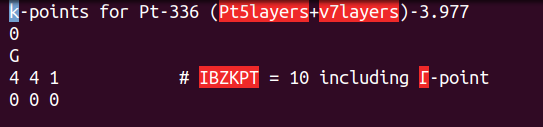
\includegraphics[height=0.4in,viewport=0 10 400 98,clip]{Figures/Pt_Slab-KPOINTS.png}
%\includegraphics[height=1.8in,width=4.in,viewport=30 210 570 440,clip]{PAW_projector.eps}
\caption{\fontsize{6.2pt}{5.2pt}\selectfont{\textrm{计算\textrm{Pt}表面时\textrm{KPOINTS}文件.}}}%(与文献\cite{EPJB33-47_2003}图1对比)
\label{Pt_Slab-KPOINTS}
\end{figure}
}
%\subsubsection{\rm{POSCAR}}
\frame
{
	\frametitle{\textrm{Pt~(111)}面\textrm{Slab}:~模型设计}
	\textrm{Pt~(111)}面\textrm{slab}的确定:\\
{\fontsize{7.5pt}{5.2pt}\selectfont{
	\begin{itemize}
		\item 根据\textrm{FCC}立方晶格参数$a$与六方晶格\textrm{HCP}参数的关系:~
\begin{displaymath}
	a_{\mathrm{HCP}}=\dfrac{a_{\mathrm{FCC}}}{\sqrt2}=\dfrac{3.977}{\sqrt 2}=2.812\mathrm{\AA}
\end{displaymath}
确定\textrm{Pt}原子的最近邻原子间距离%。\textrm{POSCAR}中共有45个\textrm{Pt}原子,按\textrm{FCC}结构的\textit{a-b-c-a-b}顺序排列。一般说,差不多当原子堆积厚度达到九层才能使\textrm{slab}内两侧表层的原子间相互作用忽略不计。不过在本次练习中,我们的模型只使用五层原子,主要是考虑到节省学习过程中的等待时间,同时也因为由此(\textrm{slab}层数过少)产生误差尚在可接受的范围内。
		\item 在\textrm{FCC-Pt}体相划出沿\textrm{(111)}的重复单元
\begin{displaymath}
	(a,0,0),~\bigg(\dfrac a2,\dfrac{\sqrt3a}2,0\bigg),~(0,0,c)
\end{displaymath}
的\textrm{Pt}原子密堆积单胞,这里$a=2.812\mathrm{\AA}$,~$c=\sqrt{8/3}a=1.633a$

用$3\times3\times6$~(含真空层)的单胞堆积得到模拟\textrm{Pt~(111)}表面的超晶胞,构成模拟\textrm{FCC}中\textrm{(111)}表面的最小重复单元
	\end{itemize}}}

为稳定\textrm{slab}模型,最底层(九个原子)完全固定,而紧邻底层(九个原子)则只在$x$和$y$方向固定。其余三层则允许在各方向弛豫%。\textrm{Pt~(111)}表面模拟使用的\textrm{POSCAR}文件如下图\ref{Pt_surface-POSCAR}所示:
}

\frame
{
	\frametitle{\textrm{Pt~(111)}面\textrm{Slab}:~模型设计}
\begin{figure}[h!]
\centering
\includegraphics[height=2.2in,viewport=0 5 540 565,clip]{Figures/Pt_surface-POSCAR.png}
%\includegraphics[height=1.8in,width=4.in,viewport=30 210 570 440,clip]{PAW_projector.eps}
\caption{\fontsize{6.2pt}{5.2pt}\selectfont{\textrm{模拟\textrm{Pt~(111)}表面时使用的\textrm{POSCAR}文件.}}}%(与文献\cite{EPJB33-47_2003}图1对比)
\label{Pt_surface-POSCAR}
\end{figure}
{\fontsize{6.2pt}{5.2pt}\selectfont{\textrm{Pt~(111)}表面是\textrm{FCC}结构下最密堆积的表面, 比\textrm{(001)}表面的原子密度要高约15\%%。计算开始之后,在最初生成的\textrm{OUTCAR}文件中,我们将能看到\textrm{Pt}原子间的最近邻距离是$2.81\mathrm{\AA}$。
}}
}

\frame
{
	\frametitle{\textrm{Pt~(111)}面\textrm{Slab}:~模型设计}
表面计算用\textrm{slab}和外加真空层来代表表面
					\begin{minipage}[t]{0.60\textwidth}
\begin{figure}[h!]
\centering
\includegraphics[height=1.9in,viewport=0 0 300 580,clip]{Figures/Pt_surface.png}
%\includegraphics[height=1.8in,width=4.in,viewport=30 210 570 440,clip]{PAW_projector.eps}
\caption{\fontsize{6.2pt}{5.2pt}\selectfont{\textrm{计算\textrm{Pt}\textrm{slab}的表面与重排.}}}%(与文献\cite{EPJB33-47_2003}图1对比)
\label{Pt_surface}
\end{figure}
					\end{minipage}
				\hfill
					\begin{minipage}[t]{0.38\textwidth}
{\fontsize{8.2pt}{5.2pt}\selectfont{注意,在\textrm{Pt~(111)}表面层,要考虑\textrm{Pt}原子发生重排问题,比如会形成六方密堆积\textrm{(Hexagonal closed-packing, HCP)}构型%,如图\ref{Pt_surface}中所示。
}}
					\end{minipage}
{\fontsize{6.2pt}{5.2pt}\selectfont{两个收敛测试:~\textrm{slab}厚度和真空厚度选择的测试}}\\%。本练习中,\textrm{Pt~(111)}表面如图\ref{Pt_surface}所示,最小重复单元由45个原子构成的\textrm{slab}外加大的真空层($\sim16\mathrm{\AA}$)构成,为的是防止表面与临近的表面间存在相互作用。
}

\frame[allowframebreaks]
{
	\frametitle{表面能的计算}
%\subsubsection{\rm{计算结果}}
%\textrm{OSZICAR}文件中记录的是弛豫过程中的\textrm{Pt~(111)}表面体系的基态能量变化情况。
%结构弛豫完全结束后,可以通过命令:\\
%\textcolor{magenta}{\textrm{grep~\`~E0~\'~OSZICAR}}\\
%来查看弛豫过程中的能量变化情况,结果如图\ref{Pt_surface-OSZICAR}所示。
\begin{figure}[h!]
\centering
\includegraphics[width=4.0in,viewport=0 0 640 108,clip]{Figures/Pt_surface-OSZICAR.png}
%\includegraphics[height=1.8in,width=4.in,viewport=30 210 570 440,clip]{PAW_projector.eps}
\caption{\fontsize{6.2pt}{5.2pt}\selectfont{\textrm{\textrm{Pt~(111)}表面计算弛豫过程中的体系能量变化(部分).}}}%(与文献\cite{EPJB33-47_2003}图1对比)
\label{Pt_surface-OSZICAR}
\end{figure}
%最后一行就是体系弛豫完成后的自由能和基态能量。
{\fontsize{7.0pt}{5.2pt}\selectfont{
%在\ref{Sec:bulk-Pt}节,我们得到体相超晶胞中的一个\textrm{Pt}原子的能量是~--6.058\textrm{~eV/atom},因此
未弛豫表面能\textrm{(the unrelaxed surface energy)},$\gamma_{\mathrm{unrel}}$可由下式确定:~
\begin{displaymath}
	\begin{aligned}
		\gamma_{\mathrm{s}}^{\mathrm{unrel}}=&\dfrac12\big(E_{\mathrm{slab}}^{\mathrm{unrel}}-NE_{\mathrm{atom}}^{\mathrm{bulk}}\big)\\
		=&\dfrac12[-261.0906-45(-6.058)] =5.76\mathrm{~eV/system}
	\end{aligned}
\end{displaymath}
表面弛豫能\textrm{(the surface relaxation energy)}可由体系完全弛豫的能量与初始能量(未经弛豫)差计算,也就是\textrm{OSZICAR}的最后一行与第一行的$E_0$差:~
\begin{displaymath}
	\gamma_{\mathrm{s}}^{\mathrm{rel}}=E_{\mathrm{last}}-E_{\mathrm{1st}}=-261.1438-(-261.0906)=-0.053\mathrm{~eV/system}
\end{displaymath}
注意表面弛豫能(也称为表面重构能)一般都比较非常小(约<1\%的表面能),而考虑底层固定的弛豫表面能\textrm{(the relaxed surface energy)}为:~
\begin{displaymath}
	5.76-0.053=5.707\mathrm{~eV/sytem}~(\mbox{即}~0.09\mathrm{~eV/\AA^2})
\end{displaymath}
该弛豫表面能与\textrm{Getman}等的高精度计算结果$0.09\mathrm{~eV/\AA^2}$%\upcite{JPC112-9559_2008}
完全一致\footnote{\fontsize{6.2pt}{5.2pt}\selectfont{另一种计算表面能的方法是固定中间层而弛豫上下表面}}
\vskip 6pt
\textrm{FCC}晶体中不同截面的原子堆垛方式不同,一般表面能按以下顺序递增:~
\begin{displaymath}
	\gamma_{111}<\gamma_{100}<\gamma_{110}
\end{displaymath}
}}
\vskip 5pt
{\fontsize{7.0pt}{5.2pt}\selectfont{对比\textrm{POSCR}和\textrm{CONTCAR}文件的晶胞参数变化,不难发现,表面层的膨胀$\sim1\%$
\vskip 10pt
在体系表面,波函数随着真空层出现,将快速衰减为零,%但计算中的平面波基组则遍及真空层和\textrm{slab},正因为此,这种
所以表面模拟的平面基数目会比普通体相计算大得多,相应的计算时长也增加得比较多(本算例中,45个原子的\textrm{slab}体系耗时6344秒),一般比体相计算的计算量大1-2倍%。本次计算没有考虑自旋极化效应,因为在超晶胞中,自旋倾向于均匀分布\footnote{所谓“均匀分布”,实质上是未成对自旋取向孤立分布,且又彼此远离,所以很难耦合形成有效磁矩}。
\vskip 10pt
对于两种固体构成的表面,如金属-金属、金属-氧化物表面,也可按类似方式处理
}}
}

%\subsection{吸附能}
\frame
{
	\frametitle{吸附能的计算}
{\fontsize{7.0pt}{5.2pt}\selectfont{
	\begin{itemize}
		\item 与表面有关的反应过程,如异相催化和化学气相沉积等,很大程度上与吸附表面的表面能有关
		\item 对于金属材料,吸附能的大小可以视为描述吸附原子轨道与金属原子的$s$-,$p$-和$d$-电子轨道的相互作用强弱的物理量
		\item 吸附能对于确定表面化学反应的反应机理至关重要%,这部分练习中,我们以简单的氧原子吸附在\textrm{Pt~(111)}表面为例,计算体系的吸附能。在\textrm{Pt~(111)}面上,有四种可能的吸附位点\textrm{(adsorption site)}:~\textrm{FCC}结构和\textrm{HCP}的间隙位\textrm{(hollow)},\textrm{Pt}原子的顶位\textrm{(top site)}和两个最近邻\textrm{Pt}原子的桥接位\textrm{(bridge site)},如图\ref{Pt_surface-site}所示。考虑到氧原子倾向于优先占据\textrm{FCC}间隙位,因此后面的计算将围绕该吸附位点进行。
	\end{itemize}}}
\begin{figure}[h!]
\centering
\includegraphics[height=2.0in,viewport=0 0 860 530,clip]{Figures/Pt_surface-site.png}
%\includegraphics[height=1.8in,width=4.in,viewport=30 210 570 440,clip]{PAW_projector.eps}
\caption{\fontsize{7.0pt}{5.2pt}\selectfont{\textrm{Pt~(111)表面俯视图,大球表示上层,小球表示下层。各吸附位见箭头标注.}}}%(与文献\cite{EPJB33-47_2003}图1对比)
\label{Pt_surface-site}
\end{figure}
}
%\subsubsection{\rm{POSCAR}}
\frame
{
	\frametitle{表面吸附建模}
%为计算固体表面吸附的气体原子或分子的吸附能,建模时要确保气体原子或分子与固体表面原子足够近,否则吸附原子或分子极易离开表面%。因此在构建\textrm{POSCAR}时,可以通过在前面计算的\textrm{Pt~(111)}表面模型得到的\textrm{CONTCAR}基础上得到吸附表面的\textrm{POSCAR}文件,如图\ref{Pt_surface-adsorption-POSCAR}所示:~
\begin{figure}[h!]
\vskip -5pt
\centering
\includegraphics[width=3.5in,viewport=0 10 520 280,clip]{Figures/Pt_surface-adsorption-POSCAR.png}
%\includegraphics[height=1.8in,width=4.in,viewport=30 210 570 440,clip]{PAW_projector.eps}
\caption{\fontsize{6.2pt}{5.2pt}\selectfont{\textrm{\textrm{Pt~(111)}表面吸附\textrm{O}的结构模型.}}}%(与文献\cite{EPJB33-47_2003}图1对比)
\label{Pt_surface-adsorption-POSCAR}
\end{figure}
%这里,总的原子数变成46个:~原有的45个\textrm{Pt}原子的\textrm{slab}模型加上一个吸附的\textrm{O}原子
{\fontsize{7.0pt}{5.2pt}\selectfont{
\textrm{O}原子坐标~$(0.55555,~0.55555,~0.37593)$~%加在文件最后一行
,这是\textrm{FCC}结构的间隙位,在空间中与三个\textrm{Pt}原子近邻。\textrm{O}原子的$z$-轴坐标根据文献报道的\textrm{Pt-O}距离确定的}}

\textrm{KPOINTS}文件与之前\textrm{Pt~(111)}表面计算相同。
}
%\subsubsection{\rm{POTCAR}}
%表面吸附计算需要的\textrm{POTCAR}文件由\textrm{Pt}和\textrm{O}各自的\textrm{POTCAR}文件拼接而成,命令如下:~\\
%\textcolor{magenta}{\textrm{cat~ POTCAR-Pt~ POTCAR-O ~ > ~POTCAR}}\\
%这里选择的是\textrm{PBE}泛函构造的原子数据集,因此用户可以通过关键词\textrm{PBE},获得有关元素和交换-相关泛函信息,如:~\\
%\textcolor{magenta}{\textrm{grep ~ \`~PBE~\' ~ POTCAR}}\\

%\subsubsection{\rm{计算结果}}
\frame
{
	\frametitle{表面吸附的计算}
%首先检查\textrm{Pt~(111)}表面吸附\textrm{O}原子的模型基态能量,命令为:\\
%\textcolor{magenta}{\textcolor{magenta}{\textrm{tail ~ nohup.out}}}\\
%结果如图\ref{Pt_surface-adsorption-nohup}所示。
	{\fontsize{7.2pt}{5.2pt}\selectfont{结构弛豫后的基态能量}}
\begin{figure}[h!]
\centering
\vskip -5pt
\includegraphics[width=4.0in,viewport=0 0 940 127,clip]{Figures/Pt_surface-adsorption-nohup.png}
%\includegraphics[height=1.8in,width=4.in,viewport=30 210 570 440,clip]{PAW_projector.eps}
\caption{\fontsize{6.2pt}{5.2pt}\selectfont{\textrm{\textrm{Pt~(111)}表面吸附\textrm{O}原子后的基态能量(部分).}}}%(与文献\cite{EPJB33-47_2003}图1对比)
\label{Pt_surface-adsorption-nohup}
\end{figure}
%查看弛豫后的\textrm{CONTCAR}文件,命令为:~\\
%\textcolor{magenta}{\textrm{cat ~ CONTCAR}}\\
%可以看出,吸附在\textrm{FCC}结构
{\fontsize{7.2pt}{5.2pt}\selectfont{间隙位的\textrm{O}原子轻度弛豫后的原子位置}}%为~(0.55555,~0.55555,~0.37598)。结果如图\ref{Pt_surface-adsorption-CONTCAR}所示:~
\begin{figure}[h!]
\centering
\vskip -5pt
\includegraphics[width=4.0in,viewport=0 0 650 95,clip]{Figures/Pt_surface-adsorption-CONTCAR.png}
%\includegraphics[height=1.8in,width=4.in,viewport=30 210 570 440,clip]{PAW_projector.eps}
\caption{\fontsize{6.2pt}{5.2pt}\selectfont{\textrm{\textrm{Pt~(111)}表面吸附\textrm{O}原子弛豫后的\textrm{O}原子位置.}}}%(与文献\cite{EPJB33-47_2003}图1对比)
\label{Pt_surface-adsorption-CONTCAR}
\end{figure}
%为了计算吸附能,还需要计算
{\fontsize{7.2pt}{5.2pt}\selectfont{孤立\textrm{O}原子能量}}%,计算方法与\ref{Sec:atom-Pt}的\textrm{Pt}原子计算方法一样。计算完毕后,可以确定孤立\textrm{O}原子的基态能量。命令为:~\\
%\textcolor{magenta}{\textrm{tail~-5~nohup.out}}\\
%结果如图\ref{O_adsorption-OSZICAR}所示:
\begin{figure}[h!]
\centering
\vskip -5pt
\includegraphics[width=4.0in,viewport=0 0 940 120,clip]{Figures/O_adsorption-OSZICAR.png}
%\includegraphics[height=1.8in,width=4.in,viewport=30 210 570 440,clip]{PAW_projector.eps}
\caption{\fontsize{6.2pt}{5.2pt}\selectfont{\textrm{孤立\textrm{O}原子的基态能量计算}.}}%(与文献\cite{EPJB33-47_2003}图1对比)
\label{O_adsorption-OSZICAR}
\end{figure}
}

\frame
{
	\frametitle{表面吸附的计算}
吸附能$E_{\mathrm{abs}}$可以通过\textrm{slab}吸附\textrm{O}原子的基态能量和洁净的\textrm{slab}与孤立原子能量差来计算:~
\begin{displaymath}
	\begin{aligned}
		E_{\mathrm{ads}}=&\dfrac1{N_{\mathrm{O}}^{\mathrm{atom}}}\big(E_{\mathrm{O/Pt~(111)}}^{\mathrm{slab}}-E_{\mathrm{Pt~(111)}}^{\mathrm{slab}}-N_{\mathrm{O}}^{\mathrm{atom}}E_{\mathrm{O}}^{\mathrm{atom}}\big)\\
		=&-267.2488-(-261.1438)-(-1.5514)\\
		=&-4.55\mathrm{~eV}
	\end{aligned}
\end{displaymath}
%需要说明的是,针对突出稳定吸附体系,
{\fontsize{7.2pt}{5.2pt}\selectfont{习惯将吸附能只取其绝对值}}%。本次计算的吸附能数值~--4.55\textrm{~eV}与\textrm{Pang}等的计算值~--4.68\textrm{~eV}\cite{ASS257-3047_2011}吻合得很好。
\footnote{\fontsize{6.2pt}{5.2pt}\selectfont{很多时候“氧的吸附能”,也会通过自由的气态\ch{O2}分子的吸附给出。在这种情况下,需要考虑到\ch{O2}成键能减半,因此计算式中的吸附能会减小至~$-1.42\mathrm{~eV}$,也就是~$-3.13\mathrm{~eV/O}$\upcite{Electrochim52-2219_2007}}}
\vskip 8pt
原子在其他的吸附位,如\textrm{HCP}的间隙位、桥接位和紧邻缺陷位,或者别的物质可能的吸附,都可以这样计算

}
%\subsection{功函数的计算与偶极校正}
\frame
{
	\frametitle{功函数与偶极校正}
%该练习是利用前面的计算结果来计算校正偶极后的功函数。
	\begin{itemize}
		\item 功函数的定义是将一个电子从固体表面的\textrm{Fermi}能级移到无穷远处(真空中)所做的功
		\item 垂直于表面$z$-轴方向的偶极,$U_{\mathrm{dipole}}$,定义为:~
\begin{displaymath}
	U_{\mathrm{dipole}}(z)=\dfrac1A\iint U_{\mathrm{dipole}}(\vec r)\mathrm{d}x\mathrm{d}y
\end{displaymath}
	\end{itemize}
经偶极校正后的功函数为$-E_{\mathrm{F}}+U_{\mathrm{dipole}}$,和表面的几何结构和特性密切相关
}

%\subsubsection\rm{{功函数的计算}}
\frame
{
	\frametitle{功函数的计算:~输入文件}
为了计算功函数,\textrm{INCAR}文件中%多五个选项,诸如
规定模型中\textrm{slab}中心的坐标位置%。内容如图\ref{Pt_surface-workfunction-INCAR}所示:~
\begin{figure}[h!]
\centering
\includegraphics[width=4.0in,viewport=0 0 680 150,clip]{Figures/Pt_surface-workfunction-INCAR.png}
%\includegraphics[height=1.8in,width=4.in,viewport=30 210 570 440,clip]{PAW_projector.eps}
\caption{\fontsize{6.2pt}{5.2pt}\selectfont{\textrm{计算\textrm{Pt}表面功函数时\textrm{INCAR}文件增加的内容.}}}%(与文献\cite{EPJB33-47_2003}图1对比)
\label{Pt_surface-workfunction-INCAR}
\end{figure}

\textrm{KPOINTS}、\textrm{POSCAR}和\textrm{POTCAR}与表面吸附算例\textrm{Pt~(111)-O}中相同。
}
%\subsubsection{\rm{功函数的计算:~计算结果}}
\frame
{
\frametitle{\rm{功函数的计算:~计算结果}}
%首先用命令查找
\textrm{OUTCAR}中的\textrm{Fermi}能级的数值:
%\textcolor{magenta}{\textrm{grep ~ fermi ~ OUTCAR}}\\
%结果如图\ref{Pt_surface-workfunction-LOCPOT}所示。
\begin{figure}[h!]
\centering
\vskip -3pt
\includegraphics[width=4.0in,viewport=0 20 460 50,clip]{Figures/Pt_surface-workfunction-Fermi.png}
%\includegraphics[height=1.8in,width=4.in,viewport=30 210 570 440,clip]{PAW_projector.eps}
\caption{\fontsize{6.2pt}{5.2pt}\selectfont{\textrm{计算\textrm{Pt}表面功函数时\textrm{Fermi}能级的数值.}}}%(与文献\cite{EPJB33-47_2003}图1对比)
\label{Pt_surface-workfunction-LOCPOT-1}
\end{figure}
%计算中产生新的
输出文件\textrm{LOCPOT}与\textrm{CHGCAR}文件格式相同\\
{\fontsize{6.2pt}{5.2pt}\selectfont{内容是三维空间中的表面平均化的局域静电势\textrm{(the planar-averaged local-electrostatic potential)},但不包含交换-相关势}}
\begin{figure}[h!]
	\vskip -5pt
\centering
\includegraphics[width=3.2in,viewport=0 10 480 250,clip]{Figures/Pt_surface-workfunction-LOCPOT.png}
%\includegraphics[height=1.8in,width=4.in,viewport=30 210 570 440,clip]{PAW_projector.eps}
\caption{\fontsize{6.2pt}{5.2pt}\selectfont{\textrm{计算\textrm{Pt}表面功函数时\textrm{LOCPOT}文件的内容.}}}%(与文献\cite{EPJB33-47_2003}图1对比)
\label{Pt_surface-workfunction-LOCPOT-2}
\end{figure}
}

\frame
{
	\frametitle{功函数的计算}
	{\fontsize{7.2pt}{5.2pt}\selectfont{为了确定$z$-方向的势函数的数值分布,应用脚本\upcite{url_plot-workfunc}处理\textrm{LOCPOT}的数据%,如本讲义附上的\textrm{Python}脚本\textcolor{blue}{\textrm{locpot\_workfunc.py}}\footnote{该软件由韩国汉城大学\textrm{Jinwoo,Park,Lanhee Yang}开发\cite{Park-Yang}},将\textrm{LOCPOT}的数值转成$\ast\mathrm{.dat}$格式的文件%,运行命令为:\\
%\textcolor{blue}{\textrm{python ~ locpot.py ~ LOCPOT ~ --0.3174}}\\
%一般习惯,\textrm{Fermi}能级$0.3174$~将会被设为0,脚本执行后的
	%输出文件\textrm{output.dat}将被用于绘制功函数图%(如图\ref{Pt_surface-workfunction}所示)。
}}
\begin{figure}[h!]
\centering
\includegraphics[height=2.0in,viewport=0 0 760 550,clip]{Figures/Pt_surface-workfunction.png}
%\includegraphics[height=1.8in,width=4.in,viewport=30 210 570 440,clip]{PAW_projector.eps}
\caption{\fontsize{6.2pt}{5.2pt}\selectfont{\textrm{计算\textrm{Pt~(111)}表面吸附\textrm{O}原子后的势函数和功函数,\textrm{Fermi}能已经置零.}}}%(与文献\cite{EPJB33-47_2003}图1对比)
\label{Pt_surface-workfunction}
\end{figure}
{\fontsize{7.2pt}{5.2pt}\selectfont{功函数图表明,\textrm{Pt~(111)}层沿$z$-轴相对\textrm{Fermi}能级位置,功函数为\textrm{5.8}\textrm{~eV}}}
}
\subsection{\rm{NEB}方法与反应过渡态搜索}
%日常经验告诉我们,两地间行走时,通常会有多条路径可供选择。如果时间有限,为及时赶到,一般会选择最短的路径;~但如果时间充裕,又想体验行走的乐趣,就可以选择更有风味的路线,如图\ref{Pt_NEB-move}所示。原子(或其物质)间因相互作用而运动时,在力驱使下,则一定会沿着能量最低的路径行走,就像俗话说的“水往低处流”。
%\begin{figure}[h!]
%\centering
%\includegraphics[width=4.0in,viewport=0 0 630 420,clip]{Pt_NEB-move.png}
%%\includegraphics[height=1.8in,width=4.in,viewport=30 210 570 440,clip]{PAW_projector.eps}
%\caption{\small \textrm{两点之间人和原子受力运动的示意图.}}%(与文献\cite{EPJB33-47_2003}图1对比)
%\label{Pt_NEB-move}
%\end{figure}
\frame
{
	\frametitle{\textrm{NEB}方法基本原理}
材料学研究中的一个基本问题是,体系如何从一个稳定态变化到另一个稳定态,也就是确定变化动力学过程的最小能量路径\textrm{(the minimum energy path, MEP)}%。本节练习中,我们学习
\vskip 5pt
{\fontsize{7.2pt}{5.2pt}\selectfont{\textrm{VASP}中采用\textrm{NEB~(Nudged elastic band)~}方法%\cite{JCP113-9978_2000,JCP113-9901_2000,JCC32-1769_2011}
来确定最小能量路径的计算过程,并确定相应的反应势垒}}
%\subsection{\rm{NEB}的基本原理}
%如图\ref{Pt_NEB}所示的
%势能面上,始态\textrm{(the initial state)}和终态\textrm{(the finial state)}分别对应势能面上的两个局域极小值。有两个典型的连线可以将这两个态关联起来:~一个是直的点线连接,另一个是最小能量曲线。由箭头所示,从直线出发,尽可能快速高效地找到最小能量曲线
\begin{figure}[h!]
	\vskip -10pt
\centering
\includegraphics[width=2.5in,viewport=0 0 770 530,clip]{Figures/Pt_NEB.png}
%\includegraphics[height=1.8in,width=4.in,viewport=30 210 570 440,clip]{PAW_projector.eps}
\caption{\fontsize{7.2pt}{5.2pt}\selectfont{\textrm{NEB}方法的基本原理:~起始时将三个假想态用直线能量路径(虚线)串联,然后向最小能带路径(实线)微动,该最小能量路径将通过各势垒的鞍点.}}%(与文献\cite{EPJB33-47_2003}图1对比)
\label{Pt_NEB}
\end{figure}
}
%\subsubsection{\rm{受力计算}}
%\subsection{NEB方法的计算过程}
%\subsubsection{\textrm{始和终态}}
\frame
{
	\frametitle{最小能量路径与假想态}
%首先,
%	一般电子和离子弛豫的时候,都确定始态和终态。在化学反应过程中,这两种构型的能量都应该是位于极小位置,各原子受力(即能量的一阶导数)也都是零。
%\subsubsection{\rm{初始能量路线}}
%既然
	最小能量路径是始态向终态变化的某一条能量路线(化学上习惯称反应通道)%,我们
	\begin{itemize}
		\item 首先用直线能量路径把两个态连接起来,以此作为尝试的能量路线,在能量路线上等距离地选择一些点(作为假想态,\textrm{images})\\%,如图\ref{Pt_NEB}所示。
			{\fontsize{7.2pt}{5.2pt}\selectfont{注意每个假想态表示的是反应过程中的一个特定的中间构型,假想态的数目则依赖于能量路线的复杂性}}%,即能量路径曲率。对于绝大部分材料,三到七个假想态已经足够。这种始态和终态连线上的假想态,可能与最小能量路径中原子构型偏差很大。显然,这种构型中的原子将受到极大的外力,计算模拟中的收敛也会很困难,常常需要一些手工的调整,使得假想态接近最小能量路径中的原子构型。
%\subsubsection{\rm{推拉能量路径}}
		\item 要求初始能量路线(直线)中的各原子构型一点点地朝原子受力为零的构型方向轻微移动\\%(类似于对一个弹性带子施以推力或拉力),就有可能搜索到最小能量路径。
			{\fontsize{7.2pt}{5.2pt}\selectfont{为控制能量路线的移动,对能量路线上的等间距分布的假想态施加沿特定方向的弹性应力,确保能量路线连续地朝最小能量路径方向过渡}}%。换句话说,
		\item 反应通道搜索过程,就是反应势能面上各原子构型落到局域极小处的过程,即每个假想态都达到最小受力构型%,如图\ref{Pt_NEB}所示。这些假想态的关系,类似于穿越沙丘的骆驼队:~每头骆驼都用缰绳彼此串在一起,保证每头骆驼都不会脱离驼队。
	\end{itemize}
}

\frame
{
	\frametitle{\textrm{NEB}方法}
\textrm{NEB}方法采用受力投影(不是能量投影):
\vskip 3pt
{\fontsize{7.2pt}{5.2pt}\selectfont{目的是确保假想态的连线能通过鞍点\textrm{(the saddle points)},达到最小能量路线}}
\begin{itemize}
	\item 初始能量连线上的每个假想态的原子受力移动的力是弹性回复力和原子间力的合力\\
		{\fontsize{7.2pt}{5.2pt}\selectfont{为了将初始能量路线直接推向最小能量路线,只考虑沿能量路线(该点切线)的弹性回复力投影和垂直能量路线(法线)的原子间作用力投影,而忽略其余力的贡献}}
	\item 通过\textrm{DFT}计算,得到每个微动过程中的原子构型的电子态极小值,并计算每个原子上的受力以确定减小受力的微动方向\\
		{\fontsize{7.2pt}{5.2pt}\selectfont{初始能量路线将会向最小能量路线移动}}
	\item 重复上述过程,直到每个原子上的受力都小于预设的接近零的小值,得到的能量路线就认为是最小能量路线
\end{itemize}
由于上述微动是根据受力推测的,因此在计算过程中,原子构型的结构弛豫算法采用\textrm{damped MD}算法(\textcolor{cyan}{\textit{IBRION}}=3)。
}

\frame
{
	\frametitle{\textrm{CI-NEB}方法}
%\subsubsection{\rm{CI-NEB}方法}
	\textrm{CI-NEB}方法是对\textrm{NEB}方法的修正%,假设是能量最高的假想态应用位于鞍点
	\vskip 5pt
{\fontsize{8.2pt}{5.2pt}\selectfont{
\begin{itemize}
%	\item 确定能量最高的假想态
	\item 最高能量的假想态位于鞍点,经过几次沿能量路线切线的微动后,不再受到弹性回复力作用\\
		{\fontsize{6.2pt}{5.2pt}\selectfont{法线方向受力将被反向(例如在原来受力方向的反向加两倍的力)}}
	\item 出现爬坡的假想态\\
		{\fontsize{6.2pt}{5.2pt}\selectfont{搜索沿能量路线上的极大值,同时又是垂直能量路线方向的极小值(即鞍点)}}
	\item 图像收敛时,将位于确切的鞍点
\end{itemize}
}}
\begin{figure}[h!]
	\vskip -15pt
\centering
\includegraphics[width=2.1in,viewport=0 0 530 450,clip]{Figures/NEB_CI-NEB.png}
%\includegraphics[height=1.8in,width=4.in,viewport=30 210 570 440,clip]{PAW_projector.eps}
\caption{\fontsize{6.2pt}{5.2pt}\selectfont{\textrm{NEB}方法与\textrm{CI-NEB}方法.}}%(与文献\cite{EPJB33-47_2003}图1对比)
\label{NEB_CI-NEB}
\end{figure}
}
%\subsection{Pt~(111)-O-NEB}
\frame
{
	\frametitle{\textrm{Pt~(111)-O-NEB}}
%以下算例说明如何
	用\textrm{NEB}方法确定\textrm{Pt~(111)}面上吸附的\textrm{O}原子由\textrm{HCP}间隙位%(如图\ref{Pt_NEB-init-POSCAR}所示)
	扩散到近邻的\textrm{FCC}间隙位的表面扩散势垒能量%。结果如图\ref{Pt_NEB-config}所示。
\begin{figure}[h!]
\centering
\includegraphics[width=4.0in,viewport=0 10 1040 530,clip]{Figures/Pt_NEB-config.png}
%\includegraphics[height=1.8in,width=4.in,viewport=30 210 570 440,clip]{PAW_projector.eps}
\caption{\fontsize{6.2pt}{5.2pt}\selectfont{\textrm{O}原子(浅灰色球)在\textrm{Pt~(111)}的\textrm{HCP}间隙位\textrm{(a)}经过中间态\textrm{(b)}扩散到最近临的\textrm{FCC}间隙位\textrm{(c)}时的原子构型变化}.}%(与 文献\cite{EPJB33-47_2003}图1对比)
\label{Pt_NEB-config}
\end{figure} 
}

%\subsubsection{\rm{Pt~(111)-slab-O-HCP}}
\frame
{
	\frametitle{\textrm{Pt~(111)-slab-O-HCP}}
采用\textrm{NEB}方法计算,首先要确定始态和终态构型的极小值%。在\ref{Sec:Surface-Pt}节我们已经确定表面吸附终态\textrm{Pt~(111)-slab-O-FCC}的构型。这里,我们将用相同的方法
%确定始态\textrm{Pt~(111)-slab-O-HCP}的构型及能量%,只是这里的\textrm{POSCAR}文件中要把\textrm{O}原子放在\textrm{HCP}的间隙位置。如图\ref{Pt_NEB-init-POSCAR}所示。
\begin{figure}[h!]
	\vskip -8pt
\centering
\includegraphics[height=2.0in,viewport=0 5 470 500,clip]{Figures/Pt_NEB-init-POSCAR.png}
%\includegraphics[height=1.8in,width=4.in,viewport=30 210 570 440,clip]{PAW_projector.eps}
\caption{\fontsize{6.2pt}{5.2pt}\selectfont{\textrm{Pt~(111)}表面\textrm{HCP}间隙位吸附\textrm{O}原子时的\textrm{POSCAR}结构文件}.}%(与文献\cite{EPJB33-47_2003}图1对比)
\label{Pt_NEB-init-POSCAR}
\end{figure}
{\fontsize{7.2pt}{5.2pt}\selectfont{计算收敛的基态能量是~$-266.87\mathrm{~eV/system}$,\textrm{NEB}计算需要的输出文件,如\textrm{CONTCAR}和\textrm{OUTCAR},可以确定始态能量极小值时的构型和原子位置}}
}

%\subsubsection{\rm{用VTST脚本运行NEB}}
\frame
{
	\frametitle{\textrm{VTST}与\textrm{NEB}计算}
	\textrm{VTST}脚本%\footnote{\fontsize{6.2pt}{5.2pt}\selectfont{\textrm{VTST:~\url{http://theory.cm.utexas.edu/vtsttools/}}}}
	是开源软件,提供有\textrm{VASP}的接口,支持\textrm{VASP}完成\textrm{NEB}计算%。下载\textrm{VTST}后,将源文件解压到\textrm{VASP}的源代码目录下,并用\textrm{make}命令编译全部$\ast.\mathrm{F}$文件(包括\textrm{neb.F},\textrm{dynamt.F}等)得到新的可执行\textrm{NEB}版\textrm{VASP}。为了实现\textrm{NEB}计算,在
%\textrm{INCAR}文件中,除了修改必要的离子弛豫参数\textit{IBRON}=3外,额外增加3个参数\textit{IMAGES}=1,\textit{SPRING}=-5.0,\textit{LCLIMB}=\textrm{.TRUE.}%。如图\ref{Pt_NEB-INCAR}所示。
\begin{figure}[h!]
\centering
\includegraphics[width=4.0in,viewport=0 0 630 200,clip]{Figures/Pt_NEB-INCAR.png}
%\includegraphics[height=1.8in,width=4.in,viewport=30 210 570 440,clip]{PAW_projector.eps}
\caption{\fontsize{6.2pt}{5.2pt}\selectfont{\textrm{VASP}计算\textrm{NEB}计算时需要新增的\textrm{INCAR}选项.}}%(与文献\cite{EPJB33-47_2003}图1对比)
\label{Pt_NEB-INCAR}
\end{figure}
注意假想态的数目要与\textrm{CPU}的数目匹配,每个假想态要均衡地分配到\textrm{CPU}上去计算%,以\textrm{CPU}数为8为例,假想态数目可选为1,2,4或8。脚本会在计算目录下新建目录,并将前述两类计算得到的\textrm{CONTCAR}文件复制到该目录下,并分别重命名为\textrm{CONTCAR1}(始态,\textrm{O}位于\textrm{HCP}间隙位)和\textrm{CONTCAR}(终态,\textrm{O}位于\textrm{FCC}间隙位)。由于本算例是简单的直接扩散,所以可以只用一个假想态,\textrm{VTST}将采用线性插值为中间假想态生成\textrm{POSCAR}文件。命令为:~\\
}

\frame
{
	\frametitle{\textrm{VTST}与\textrm{NEB}计算}
{\fontsize{7.2pt}{5.2pt}\selectfont{
%\textcolor{magenta}{\textrm{$\sim$/vtstscripts/nebmake.pl~\textrm{CONTCAR1}~\textrm{CONTCAR2}~1}}\\
\textrm{VTST}脚本会产生三个目录,分别为00(始态),01(中间假想态),02(终态)%。在\textrm{POSCAR}文件中,原子位置的坐标将都会用正值表示,如$-0.001\rightarrow0.999$。其中目录00中的\textrm{OUTCAR}直接从\textrm{Pt~(111)-slab-O-HCP}中复制,类似地,目录02中的\textrm{OUTCAR}来自\textrm{Pt~(111)-slab-O-FCC}。这几个目录中的\textrm{OUTCAR}中最后得到的基态总能\textit{E0}将是计算扩散势垒的根据。计算中的\textrm{POTCAR}和\textrm{KPOINTS}也都完全相同。计算过程中,可以通过命令监控计算过程中原子受力变化的情况:\\
%\textcolor{magenta}{\textrm{grep~\`~max~atom~\'~OUTCAR}}\\

%这里第一个数是当前假想态中受力最大的原子,
当每个假想态上的原子受力低于力标准(本算例为$<0.05\mathrm{eV/\AA}$),即达到收敛%。如果起始受力太大($>10\mathrm{eV/\AA}$),就要调整为更合适的起始结构重新来计算。

%计算过程可以用脚本\textrm{vtstscript/nebef.pl}来监控,监控信息将会写到文件$\mathbf{neb}\ast\mathbf{.dat}$中。例如,经过19次和30次的离子弛豫后的数据如图\ref{Pt_NEB-VTST-1}所示:
\begin{figure}[h!]
\centering
\includegraphics[height=1.5in,viewport=0 20 300 200,clip]{Figures/Pt_NEB-VTST-1.png}
%\includegraphics[height=1.8in,width=4.in,viewport=30 210 570 440,clip]{PAW_projector.eps}
\caption{\fontsize{6.2pt}{5.2pt}\selectfont{\textrm{经过19次和30次离子弛豫后的数据.}}}%(与文献\cite{EPJB33-47_2003}图1对比)
\label{Pt_NEB-VTST-1}
\end{figure}

这里所有数据按假想态的顺序排列,分别是力,基态总能以及基态总能与起始态的能量差%。所有的数据文件(如\textrm{OUTCAR}、\textrm{WAVECAR}、\textrm{CHGCAR}等)都写到01目录内。一般
一个\textrm{VTST}计算得到稳定的鞍点假想态,需要比较长的时间,因为这个假想态是亚稳态,非常不稳定}}
}

%\subsubsection{计算结果}
\frame
{
	\frametitle{\textrm{Pt~(111)-slab-O-扩散曲线}}
%脚本\textrm{nebbarrier.pl}输出的是反应坐标,即以能量路线上各假想态为横坐标,计算各假想态基态总能的能量差和每个假想态的原子的最大受力。 而脚本\textrm{nebresults.pl}执行后则输出一系列的后处理数据文件。
{\fontsize{7.2pt}{5.2pt}\selectfont{
原子从\textrm{Pt~(111)}的\textrm{HCP}的间隙位移动到\textrm{FCC}间隙位时,原子构型对相应基态总能差的曲线数据(即反应通道)
\begin{figure}[h!]
\centering
\includegraphics[height=1.0in,viewport=0 0 300 80,clip]{Figures/Pt_NEB-VTST-2.png}
%\includegraphics[height=1.8in,width=4.in,viewport=30 210 570 440,clip]{PAW_projector.eps}
\caption{\fontsize{6.2pt}{5.2pt}\selectfont{\textrm{NEB}计算的反应坐标数据.}}%(与文献\cite{EPJB33-47_2003}图1对比)
\label{Pt_NEB-VTST-2}
\end{figure}
%图\ref{Pt_NEB-energydiff}表明
	该反应路径中正向扩散势垒为0.155\textrm{eV},反向扩散,即从\textrm{FCC}间隙位扩散到\textrm{HCP}间隙位,其势垒则为0.53\textrm{eV},这和%\textrm{Pang}等的
	计算值(0.5\textrm{eV})%\upcite{ASS257-3047_2011}
	吻合得很好,与实验值(0.43\textrm{eV})%\upcite{PRL77-123_1996}
也比较一致}}
\vskip 5pt
结果表明,中等强度的热扰动就可以将吸附在\textrm{Pt~(111)}面上\textrm{HCP}间隙位的\textrm{O}原子扩散到\textrm{FCC}间隙位上%。本次练习的计算流程可以推广到双金属\textrm{slab}\cite{PRL81-2819_1998}中的芯-壳纳米团簇体系的应力结构研究等相关理论计算中去。
}

\frame
{
	\frametitle{\textrm{Pt~(111)-slab-O-扩散曲线}}
\begin{figure}[h!]
\centering
\includegraphics[height=2.5in,viewport=0 0 790 640,clip]{Figures/Pt_NEB-energydiff.png}
%\includegraphics[height=1.8in,width=4.in,viewport=30 210 570 440,clip]{PAW_projector.eps}
\caption{\fontsize{6.2pt}{5.2pt}\selectfont{\textrm{CI-NEB}方法计算的反应势垒.}}%(与文献\cite{EPJB33-47_2003}图1对比)
\label{Pt_NEB-energydiff}
\end{figure}
}

\subsection{{\rm Pt~(111)}表面催化计算}
\frame
{
	\frametitle{催化剂与催化反应}
%\subsection{催化剂}
	\textcolor{magenta}{催化剂}:~能够改变化学反应进程(一般是加速反应完成,也有少数催化剂是减缓反应过程),但\textcolor{red}{在反应前、后不改变物质组分的物质}%。如图\ref{Pt_NEB-reaction}所示,
\vskip 3pt
{\fontsize{7.2pt}{5.2pt}\selectfont{
对于一个给定化学反应,由于催化剂的存在,降低了活化能,为反应过程提供了新的反应通道,但反应的自由能($\Delta G$)不变
\vskip 5pt
\textcolor{blue}{催化剂的存在,虽然改变了化学反应的动力学学过程,但不改变化学反应的热力学过程}}}%图示的催化剂的概念很简单,但是在实际的反应过程,会涉及大量的化学结构和电子态的变化,故此一般催化反应过程都相当复杂。
\begin{figure}[h!]
\centering
\includegraphics[height=1.7in,viewport=0 0 850 660,clip]{Figures/Pt_NEB-reaction.png}
%\includegraphics[height=1.8in,width=4.in,viewport=30 210 570 440,clip]{PAW_projector.eps}
\caption{\fontsize{6.2pt}{5.2pt}\selectfont{催化剂的存在对反应通道的能量影响(反应通道)的示意图.}}%(与文献\cite{EPJB33-47_2003}图1对比)
\label{Pt_NEB-reaction}
\end{figure} 
}

\frame
{
	\frametitle{催化剂与态密度\textrm{DOS}}
%不难理解,
	催化剂表面与吸附介质相互作用的细节对于深入认知催化反应过程非常关键%\textrm{DFT}方法已经成为寻找更优异的催化材料的高效手段,并且为解释实验结果,并能提供实验难以或无法提供的细节。本节中通过对态密度\textrm{(Density of States, DOS)}的
	\vskip 5pt
	{\fontsize{6.2pt}{5.2pt}\selectfont{研究中通过态密度来表征催化表面的电子结构的改变}}
%\subsection{态密度}
%对周期体系,在每个$\vec k$点上都要通过自洽迭代来求解\textrm{Kohn-Sham}方程,得到\textrm{Kohn-Sham}本征态轨道和能量本征值(一般称为单电子本征态)。电子结构的表示有两种重要的方式,也就是能带结构和\textrm{DOS}。一般能带结构都是沿着不可约\textrm{Brillouin}区中的高对称性线方向绘制。而\textrm{DOS}则表示的是整个\textrm{Brillouin}区的电子态的数目。

%\textrm{DOS}反映的是电子态在$\vec k$空间的分布状况,定义为通过单位能量范围内的电子态的数目:
%\begin{equation}
%	\begin{aligned}
%		D(\varepsilon)=&\dfrac{\mbox{能量}\varepsilon\mbox{和}\partial\varepsilon\mbox{之间的态的数目}}{\partial\varepsilon}\\
%		=&2\sum_{\vec k}\delta[\varepsilon-\varepsilon_n(\vec k)]
%	\end{aligned}
%	\label{eq:DOS}
%\end{equation}
%在特定能级附近的高态密度意味着在这个能量附近有很多占据态。如果对态密度积分,积分到\textrm{Fermi}能级,可以得到体系的电子数:~
%\begin{equation}
%	n=\int_0^{E_{\mathrm{F}}}D(\varepsilon)\mathrm{d}\varepsilon
%	\label{eq:DOS-integral}
%\end{equation}

%\subsection{Pt~(111)-slab-O-DOS计算}
%\subsubsection{\rm{静态计算}}
%弛豫计算结束,开始静态计算时,将在\textrm{INCAR}中设参数\textit{NSW}=0,并将\textrm{CONTCAR}和\textrm{CHGCAR}作为静态自洽的结构和初始电荷密度的起点。此外,要把\textrm{KPOINTS}中的$\vec k$点增加为$6\times6\times1$,以保证计算计算精度。
%\subsubsection{\rm{DOS}计算}
%静态计算之后是根据当前得到的电荷密度\textrm{CHGCAR}进行非自洽计算(物性计算),要将\textrm{INCAR}中设置参数\textit{ICHARG}=11。如图\ref{Pt_surface-DOS-INCAR}所示。
\begin{figure}[h!]
\centering
\includegraphics[height=0.9in,viewport=0 0 500 120,clip]{Figures/Pt_surface-DOS-INCAR.png}
%\includegraphics[height=1.8in,width=4.in,viewport=30 210 570 440,clip]{PAW_projector.eps}
\caption{\fontsize{6.2pt}{5.2pt}\selectfont{\textrm{静态计算最主要的任务之一:~\textrm{DOS}计算时的\textrm{INCAR}设置.}}}%(与文献\cite{EPJB33-47_2003}图1对比)
\label{Pt_surface-DOS-INCAR}
\end{figure}
%这样的参数设置会在计算过程中将保持基态电荷密度和势不变,最后得到每个$\vec k$点上的电子本征态
%有时我们需要将\textrm{DOS}中的部分投影出来。
	态密度的投影可以分为针对轨道、原子、元素或\textrm{slab}的层等等多种投影,称为投影态密度(或分波态密度)%。在实验技术中,固体的态密度一般通过光电子发射谱测量。
}
%\subsubsection{\rm{计算结果}}

\frame
{
	\frametitle{\textrm{Pt~(111)}表面催化计算:~态密度}
{\fontsize{8.5pt}{5.2pt}\selectfont{
	\begin{itemize}
		\item \textrm{DOSCAR}:~给出体系的态密度和积分态密度\textrm{(the integrated DOS)}%(单位:~态数目/\textrm{unit cell}),如图\ref{Pt_PDOS-d}所示。而
		\item \textrm{PROCAR}:~给出每个能带的轨道按轨道分量~$s$-,~$p$-,~$d$-,~$f$-~投影的情况
	\end{itemize}}}
\begin{figure}[h!]
\centering
\includegraphics[height=2.2in,viewport=0 20 830 620,clip]{Figures/Pt_PDOS-d.png}
%\includegraphics[height=1.8in,width=4.in,viewport=30 210 570 440,clip]{PAW_projector.eps}
\caption{\fontsize{6.2pt}{5.2pt}\selectfont{\textrm{Pt(111)中的\textrm{Pt}的\textit{d}轨道对\textrm{DOS}的贡献}.}}%(与文献\cite{EPJB33-47_2003}图1对比)
\label{Pt_PDOS-d}
\end{figure}
}

\frame
{
	\frametitle{\textrm{Pt~(111)}表面催化计算:~投影态密度}
%我们还要将计算文件中的数据经人工提取和必要处理才能进行分析,当然这可以借助脚本完成(比如这里用的就是\textcolor{blue}{\textrm{dos.py}})。处理后得到一列能量数据和对应的每个轨道的分解占据情况。在本算例中,对\textrm{DOS}的投影:~成键原子的贡献来自\textrm{Pt}原子和\textrm{O}原子

%根据数据文件绘制\textrm{DOS}图,还需要知道体系的\textrm{Fermi}能级。命令如下:\\
%\textcolor{magenta}{\textrm{grep~fermi~OUTCAR}}\\
%将上述分波\textrm{DOS}的数据文件\textrm{pdos-Pt-O-46O.dat}导入\textrm{Xmgrace},\textrm{MS}~\textrm{Excel}或\textrm{ORIGIN}等数据绘图软件中,第一列指定为绘图时的横坐标,并以\textrm{Fermi}能级为能量原点,可以得到效果如图\ref{Pt_surface_PDOS}所示的态密度图。此外还可以画出净的\textrm{Pt}\textrm{slab}的分态密度。这里将总的态密度投影到各原子上表示为分态密度,并给出
	根据\textrm{Pt}的$d$-\textrm{DOS}和\textrm{O}的$p$-DOS,可以定性地估计两种原子的成键的键强度:~\\
%	{\fontsize{6.2pt}{5.2pt}\selectfont{\textrm{Pt-O}成键主要来自\textrm{Pt}-5\textit{d}和\textrm{O}-2\textit{p}轨道的杂化}}
\begin{figure}[h!]
\centering
\includegraphics[height=2.1in,viewport=0 0 820 620,clip]{Figures/Pt_surface_PDOS.png}
%\includegraphics[height=1.8in,width=4.in,viewport=30 210 570 440,clip]{PAW_projector.eps}
\caption{\fontsize{6.2pt}{5.2pt}\selectfont{\textrm{Pt(111)-O}体系的\textrm{PDOS}贡献:~来自\textrm{Pt}-$5d$和\textrm{O}-$2p$轨道.}}%(与文献\cite{EPJB33-47_2003}图1对比)
\label{Pt_surface_PDOS}
\end{figure}
}
\subsection{{\rm Si}的声子计算}
\frame
{
	\frametitle{\textrm{Si}的声子计算:~初基原胞}
声子描述的固体晶格振动,其特征频率$\omega(\vec q)$是量子化的%。晶格中的原子有序排列,类似于弹簧串联的小球,一个(或多个)原子偏离平衡位置引起的振动,通过“弹簧”传递,会引起一系列的原子产生类似运动,根据晶格动力学理论就产生了力常数\textrm{(force constants)}、动力学矩阵\textrm{(dynamic matrix)}等物理量。根据这些物理量,我们就可以绘制出声子在第一\textrm{Brillouin}区的频率分布$\omega(\vec q)$在$\vec k$空间的色散关系,对于具体的固体研究,声子色散关系非常重要。
%这里我们学习以\textrm{Si}为例计算简单的声子方式。实验技术中,一般通过中子散射确定固体中的声子分布。
%\subsection{\rm{构建输入文件}}
%根据\textrm{Si}的初基原胞,首先构造\textrm{POSCAR}文件如图\ref{Si_phonon-POSCAR_primitve}所示:~
\begin{figure}[h!]
\centering
\includegraphics[height=1.2in,viewport=0 0 520 160,clip]{Figures/Si_phonon-POSCAR_primtive.png}
%\includegraphics[height=1.8in,width=4.in,viewport=30 210 570 440,clip]{PAW_projector.eps}
\caption{\fontsize{6.2pt}{5.2pt}\selectfont{\textrm{用于声子计算的\textrm{Si}的初基原胞的\textrm{POSCAR}文件.}}}%(与文献\cite{EPJB33-47_2003}图1对比)
\label{Si_phonon-POSCAR_primitve}
\end{figure}
%在此基础上,
{\fontsize{7.2pt}{5.2pt}\selectfont{声子计算除了\textrm{VASP}软件,还要用到开源声子计算程序\textrm{phonopy}\upcite{Phonopy}:\\
\vskip 3pt
	通过\textrm{phonopy}程序生成若干超晶胞(如$2\times2\times2$超晶胞),%命令如下:~\\
%\textcolor{blue}{\textrm{phonopy~-d~--dim=~\`\`~2~2~2~\'\'}}\\
%该命令
将产生三组文件,包括\textrm{SPOSCAR},\textrm{DISP}和\textrm{POSCAR}-\{\textrm{number}\}}\\
{\fontsize{6.2pt}{5.2pt}\selectfont{其中\textrm{SPOSCAR}保存理想超晶胞结构,\textrm{DISP}记录各方向的原子偏离信息,而\textrm{POSCAR}-\{\textrm{number}\}是超晶胞中原子发生偏离后的位置}}
\vskip 4pt
将初基原胞\textrm{POSCAR}重命名为\textrm{POSCAR1},而\textrm{SPOSCAR}重命名为\textrm{POSCAR}}%:~\\
%\textcolor{magenta}{\textrm{mv~POSCAR~POSCAR1}}\\
%\textcolor{magenta}{\textrm{mv~SPOSCAR~POSCAR}}
}

\frame
{
	\frametitle{\textrm{Si}的声子计算:~输入文件}
	{\fontsize{7.2pt}{5.2pt}\selectfont{准备\textrm{VASP}计算需要的输入文件,开启静态计算}}%\textrm{INCAR}文件和\textrm{KPOINTS}文件,分别如图\ref{Si_phonon-INCAR},\ref{Si_phonon-KPOINTS}所示:~
\begin{figure}[h!]
\centering
\includegraphics[width=4.0in,viewport=0 0 640 110,clip]{Figures/Si_phonon-INCAR.png}
%\includegraphics[height=1.8in,width=4.in,viewport=30 210 570 440,clip]{PAW_projector.eps}
\caption{\fontsize{6.2pt}{5.2pt}\selectfont{\textrm{用于声子计算的\textrm{Si}的输入参数控制\textrm{INCAR}文件.}}}%(与文献\cite{EPJB33-47_2003}图1对比)
\label{Si_phonon-INCAR}
\end{figure}
\begin{figure}[h!]
\centering
\vskip -20pt
\includegraphics[height=0.9in,viewport=0 20 160 130,clip]{Figures/Si_phonon-KPOINTS.png}
%\includegraphics[height=1.8in,width=4.in,viewport=30 210 570 440,clip]{PAW_projector.eps}
\caption{\fontsize{6.2pt}{5.2pt}\selectfont{\textrm{用于声子计算的\textrm{Si}的$\vec k$空间布点\textrm{KPOINTS}文件.}}}%(与文献\cite{EPJB33-47_2003}图1对比)
\label{Si_phonon-KPOINTS}
\end{figure}
%根据上述输入文件,可以。
{\fontsize{7.2pt}{5.2pt}\selectfont{\textrm{VASP}计算结束,将会产生\textcolor{blue}{\textrm{DYNMAT}}文件}}
}

\frame
{
	\frametitle{\textrm{Si}的声子计算:~\textrm{Phonopy}处理}
%\subsection{声子计算}
%用以下命令可由该文件
	{\fontsize{8.0pt}{5.2pt}\selectfont{
	\begin{enumerate}
		\item 提取出力常数数据:\\
\textcolor{blue}{\textrm{phonopy~--fc~vasprun.xml}}\\
{\fontsize{6.2pt}{5.2pt}\selectfont{会生成\textcolor{blue}{\textrm{FORCE\_CONSTANTS}}文件}}
%下一步\textrm{phonopy}的输入文件\textrm{INPHON}文件中会涉及该文件。
%\subsubsection{\rm{INPHON}}
\item 准备\textrm{Phonopy}控制文件\textcolor{blue}{\textrm{INPHON}}%内容如图\ref{Si_phonon-INPHON}所示:~
\begin{figure}[h!]
\centering
\includegraphics[width=3.8in,viewport=0 0 810 140,clip]{Figures/Si_phonon-INPHON.png}
%\includegraphics[height=1.8in,width=4.in,viewport=30 210 570 440,clip]{PAW_projector.eps}
\caption{\fontsize{6.2pt}{5.2pt}\selectfont{\textrm{用于声子计算的\textrm{Si}的控制\textrm{INPHON}文件.}}}%(与文献\cite{EPJB33-47_2003}图1对比)
\label{Si_phonon-INPHON}
\end{figure}
\item 将\textrm{POSCAR}重命名为\textrm{POSCAR}$2\times2\times2$,\textrm{POSCAR1}重命名为\textrm{POSCAR}
\item 执行声子计算:~\\
\textcolor{blue}{\textrm{phonopy~-p}}\\
{\fontsize{6.2pt}{5.2pt}\selectfont{会产生绘制声子色散关系图所需的文件:~\textcolor{blue}{\textrm{band.yaml}}}}
\item 绘制声子色散关系图,执行以下命令:~\\
\textcolor{blue}{\textrm{bandplot~band.yaml}}\\
%{\fontsize{6.2pt}{5.2pt}\selectfont{绘制声子色散关系图}}
	\end{enumerate}
}}
}
%注意\textrm{bandplot}命令与\textrm{phonopy}在同一个执行目录\textrm{bin}下,运行后会产生弹出式窗口如图\ref{Fig:Si_pop-out_screen}所示。最后,\textrm{Si}在$2\times2\times2$超晶胞的声子色散分布如图\ref{Fig:Si_phonon}所示,。
\frame
{
	\frametitle{\textrm{Si}的声子谱}
\begin{figure}[h!]
\centering
\includegraphics[width=4.0in,viewport=0 0 1050 650,clip]{Figures/Si_pop-out_screen.png}
%\includegraphics[height=1.8in,width=4.in,viewport=30 210 570 440,clip]{PAW_projector.eps}
\caption{\fontsize{6.2pt}{5.2pt}\selectfont{\textrm{运行\textrm{bandplot}时的弹出界面.}}}%(与文献\cite{EPJB33-47_2003}图1对比)
\label{Fig:Si_pop-out_screen}
\end{figure}
}

\frame
{
	\frametitle{\textrm{Si}的声子谱}
%为了表明计算收敛的必要性,$3\times3\times3$和$4\times4\times4$超晶胞的结果也和$2\times2\times2$的结果列在同一张图中,
%结果表现出了更低的声学支和更高的光学支振动
\begin{figure}[h!]
	\vskip -12pt
\centering
\includegraphics[height=2.4in,viewport=0 0 780 600,clip]{Figures/Si_phonon.png}
%\includegraphics[height=1.8in,width=4.in,viewport=30 210 570 440,clip]{PAW_projector.eps}
\caption{\fontsize{6.2pt}{5.2pt}\selectfont{不同的超晶胞计算的\textrm{Si}的声子谱曲线.}}%(与文献\cite{EPJB33-47_2003}图1对比)
\label{Fig:Si_phonon}
\end{figure}
{\fontsize{7.2pt}{5.2pt}\selectfont{有了声子谱的基本数据,就可以估计晶体的熵、自由能和热膨胀等热力学数据}}%。当然,这些内容已经超出本讲义的范围,兹不赘言。
}

		\frame[allowframebreaks]
{
\frametitle{主要参考文献}
\begin{thebibliography}{99}
{\tiny
	\bibitem{PRB78-205302_2008}\textrm{H. Bentmann and A. A. Demkov and R. Gregory and S. Zollner. \textit{Phys. Rev. B} \textbf{78} (2008), 205302}
	\bibitem{Landolt-Bornstein}\textrm{Landolt-B\"ornstein, \textit{Structure Data of Elements and Intermetallic Phase},~Springer Inc.}, \textrm{(1991)}
	\bibitem{PSSA102-47_1987}\textrm{H. E. Sch\"afer. \textit{Phys. Status Solidi A} \textbf{102} (1987), 47}
	\bibitem{PRB66-214110_2002}\textrm{T. R. Mattson and A. E. Mattson. \textit{Phys. Rev. B} \textbf{66} (2002), 214110}
	\bibitem{JNM383-244_2009}\textrm{S.-C. Lee, J.-H. Choi and J. G. Lee. \textit{J. Nuclear Mat.} \textbf{383} (2009), 244}
	\bibitem{JMS44-1828_2009}\textrm{J. H. Kim, Y. D. Kwon, P. Yonathan,I. Hidayat,J. G. Lee, J.-H. Choi and S.-C. Lee. \textit{J. Matt. Sci.} \textbf{44} (2009), 1828}
	\bibitem{Electrochim52-2219_2007}\textrm{M. C. Lischka, C Mosch and A. Gro$\beta$. \textit{Electrochim. Acta..} \textbf{52} (2007), 2219}
	\bibitem{url_plot-workfunc}\url{https://gist.github.com/Ionizing/1ac92f98e8b00a1cf6f16bd57694ff03}
	\bibitem{Phonopy}\url{http://phonopy.sourceforge.net/}
	\bibitem{PRB52-R5467_1995}\textrm{A. I. Liechtenstein, V. I. Anisimov and J. Zaanen., \textit{Phys. Rev.} B, \textbf{52} (1995), R5467}
	\bibitem{PRB57-1505_1998}\textrm{S. L. Dudarev, G. A. Botton, S. Y. Savrasov, C. J. Humphreys and A. P. Sutton., \textit{Phys. Rev.} B, \textbf{57} (1998), 1505}
	\bibitem{PRB73-045112_2006}\textrm{M. Gajdo$\check{s}$, K. Hummer, G. Kresse, J. Furthm\"uller and F. Bechstedt. \textit{Phys. Rev.} B, \textbf{73} (2006), 045112}
%	\bibitem{url_p4vasp}\url{https://github.com/orest-d/p4vasp}
%	\bibitem{url_VESTA}\url{https://jp-minerals.org/vesta/en/}
		\bibitem{J.-G._Lee}\textcolor{blue}{\textrm{VASP}的算例可参考文献:%~\upcite{J.-G._Lee}
}\\ \textrm{J.-G. Lee, \textit{Computational Materials Science:~an introduction}}~\textrm{(2nd Edition),~CPC Press}, \textrm{(2017)}
		\bibitem{VASP_tutorial}\textcolor{blue}{\textrm{VASP}官网教程中的算例:%~\upcite{VASP_tutorial}
}\\ \url{https://www.vasp.at/wiki/index.php/Category:Examples}
%	\bibitem{Electrochim52-2219_2007}\textrm{M. C. Lischka, C Mosch and A. Gro$\beta$. \textit{Electrochim. Acta..} \textbf{52} (2007), 2219}
%	\bibitem{url_plot-workfunc}\url{https://gist.github.com/Ionizing/1ac92f98e8b00a1cf6f16bd57694ff03}
%	\bibitem{Phonopy}\url{http://phonopy.sourceforge.net/}
%	\bibitem{PRB52-R5467_1995}\textrm{A. I. Liechtenstein, V. I. Anisimov and J. Zaanen., \textit{Phys. Rev.} B, \textbf{52} (1995), R5467}
%	\bibitem{PRB57-1505_1998}\textrm{S. L. Dudarev, G. A. Botton, S. Y. Savrasov, C. J. Humphreys and A. P. Sutton., \textit{Phys. Rev.} B, \textbf{57} (1998), 1505}
%	\bibitem{PRB73-045112_2006}\textrm{M. Gajdo$\check{s}$, K. Hummer, G. Kresse, J. Furthm\"uller and F. Bechstedt. \textit{Phys. Rev.} B, \textbf{73} (2006), 045112}
}
\end{thebibliography}
}

\section{分子动力学基础}
\frame
{
	\frametitle{分子模拟}
	分子模拟:~\textcolor{blue}{研究原子分子层次的物性}
	\begin{itemize}
		\item 分子模拟方法分为~\textrm{Monte~Carlo~(MC)}和\textrm{Molecular~Dynamics~(MD)}两大类
		\item \textcolor{blue}{统计物理}是理论基础:~\textrm{Boltzmann}分布的重要性采样
	\end{itemize}
	\begin{itemize}
		\item 量子效应只有在粒子波长$\lambda$与原子间距离\textrm{(1-3~\AA)}相当时才变得重要:~\textcolor{blue}{一般原子/分子的运动,用经典力学足以精确描述}
			\vskip 2pt
			尽管第一性原理方法在功能材料,特别是光电磁相关研究领域中独树一帜,但是大多数与原子/分子运动相关的材料——\textcolor{blue}{典型的如结构材料}——研究,主要应用经典力学预测%特别是对于结构材料,如何利用分子动力学方法来描述材料中的原子运动是该领域的重要主题。
		\item 自\textrm{1950}年代,\textrm{Alder}和\textrm{Wainwright}通过密堆积球出发,成功模拟液-固相变%\upcite{JCP27-1208_1957}
			开始,标志着分子动力学方法成功应用到材料学模拟中
			%自此以后,大量的高效算法和代码以及不断升级的计算能力使得分子动力学在材料领域发挥的作用日益凸显,进入21世纪,\textrm{Kadau}等实现了对3200亿个原子的分子动力学模拟\cite{IJMPC17-1755_2006},显示出该方法的巨大能力。
	\end{itemize}
	分子模拟:~\textcolor{red}{计算材料研究领域最重要的理论工具之一}
}

\frame
{
	\frametitle{\textrm{Monte~Carlo}模拟}
\begin{minipage}{0.33\textwidth}
%\begin{figure}[h!]
%\centering
%\vspace{-8.0pt}
%\includegraphics[height=1.45in,width=1.50in,viewport=0 0 140 138,clip]{Figures/Unit_Cell_of_Liquid_Water.png}
%\caption{\textrm{\tiny Schematic representation of water can be simulated using Periodic Boundary Conditions.}}
%\label{Water-PBC}
%\end{figure}
\begin{itemize}
\vspace{-8.0pt}
{\fontsize{9.5pt}{6.2pt}\selectfont{
	\item 基于\textrm{Boltzmann}分布,只能模拟平衡态体系
	\item 只计算势能(状态函数),不用计算力(瞬时作用)
\item 模拟步长可以比较大}}
\end{itemize}
\end{minipage}
\begin{minipage}{0.65\textwidth}
\begin{figure}[h!]
\centering
\vspace{-5.0pt}
\includegraphics[height=1.55in,width=3.00in,viewport=0 0 930 475,clip]{Figures/Schematic-representation-of-the-Metropolis-Monte-Carlo-simulation.png}
%\caption{\textrm{Schematic representation of the Metropolis−Monte Carlo simulation.}}
\label{MC-Algorithm-Workflow}
\end{figure}
\end{minipage}
\begin{figure}[h!]
\centering
\vspace{-10.0pt}
\includegraphics[height=1.25in,width=4.15in,viewport=0 0 1470 480,clip]{Figures/Monte-Carlo-development.png}
%\caption{\textrm{Schematic representation of the Metropolis−Monte Carlo simulation.}}
\label{Monte-Carlo-development}
\end{figure}
}

\subsection{经典分子动力学提要}
\frame
{
	\frametitle{}
\begin{figure}[h!]
\centering
\vspace{-7.0pt}
\includegraphics[height=2.85in,width=3.80in,viewport=0 0 410 300,clip]{Figures/Nobel_Prize_Chemistry-2013.jpg}
%\caption{\textrm{Schematic representation of the Metropolis−Monte Carlo simulation.}}
\label{Nobel-Prize-Chemistry_2013}
\end{figure}
}

\frame
{
	\frametitle{经典分子动力学}
\begin{minipage}{0.45\textwidth}
\begin{figure}[h!]
\centering
\vspace{-3.0pt}
\includegraphics[height=2.00in,width=2.00in,viewport=0 0 135 135,clip]{Figures/Unit_Cell_of_Liquid_Water.png}
%\caption{\textrm{Schematic representation of the Metropolis−Monte Carlo simulation.}}
\label{Unit_Cell_of_Liquid_Water}
\end{figure}
\end{minipage}
\begin{minipage}{0.53\textwidth}
	\begin{itemize}
		\item 应用数值方法解析多粒子体系(原子、离子、$\cdots$)运动
		\item 粒子间相互作用可用简洁的解析函数或数值描述
		\item 广泛应用于材料科学、物理化学和生物科学的相关研究
		\item 模拟体系的粒子数规模:~\\$100\sim10^6$
		\item 模拟体系的时间范围:~\\$10~\mathrm{ps}\sim1\mu\mathrm{s}$~(一般是$\mathrm{ns}$范围)
	\end{itemize}
\end{minipage}
\begin{itemize}
	\item 分子动力学模拟可以包括温度和压力效应
	\item 分子动力学可以模拟相对大的体系和相对长的时间
	\item 分子动力学可以得到分子尺度的结构和动力学信息
\end{itemize}
}

\frame
{
	\frametitle{经典分子动力学}
	分子动力学方法的\textcolor{red}{优点}:
	\begin{itemize}
			\setlength{\itemsep}{5pt}
		\item 可以模拟大规模分子系统,原则上能计算系统的微观、宏观物理量,增补实验数据的空缺
		\item 与\textrm{Monte Carlo}方法相比,具备更高的准确度,可以提供更多微观粒子的运动细节
		\item 可以模拟非平衡态的体系以及体系在极端条件下复杂情况下的物理性质和物理状态
	\end{itemize}
	分子动力学方法的\textcolor{red}{缺点}:
	\begin{itemize}
			\setlength{\itemsep}{5pt}
		\item 只能描述原子(核)的运动,但无法反映电子的运动,难以准确模拟化学键
		\item 数值模拟依赖经验力场,化学环境复杂的体系,如化学键断裂,电子结构将由稳态电子结构过渡到过渡态,无法用简单的解析力场描述
	\end{itemize}
}

\frame
{
	\frametitle{经典力学\textrm{Classical Mechanics}}
\begin{figure}[h!]
\vspace*{-0.18in}
\centering
\includegraphics[height=2.65in,width=4.05in,viewport=0 0 715 495,clip]{Figures/Classical_Mechanics.jpg}
%\includegraphics[height=2.50in,width=4.05in,viewport=0 20 735 470,clip]{Figures/Two-dark-cloud-in-physics-3.jpg}
%\includegraphics[height=2.40in,width=4.05in,viewport=0 50 735 470,clip]{Figures/Two-dark-cloud-in-physics-2.jpg}
%\includegraphics[height=2.40in,width=4.05in,viewport=0 0 580 325,clip]{Figures/Two-dark-cloud-in-physics-1.jpg}
\label{Classical_Mechanics}
\end{figure}
}

\frame
{
	\frametitle{\textrm{\small Newtonian, Lagrangian and Hamiltonian Mechanics}}
	\begin{itemize}
   		\setlength{\itemsep}{10pt}
		\item \textrm{\textcolor{blue}{Newtonian~Mechanics}}\\
		牛顿运动定律体系是以力、加速度、动量这些矢量为基本量来描述力学系统在欧氏空间的运动~(用几何方程表述约束)
	\item \textrm{\textcolor{blue}{Lagrangian~Mechanics}}\\
		拉格朗日力学是关于研究对象在其对应的约束系统下的运动形式,大大压缩牛顿方程描述需要的约束个数。不需要在另外设未知数目
	\item \textrm{\textcolor{blue}{Hamiltonian~Mechanics}}\\
		哈密度力学由拉格朗日力学演变而来,把位置和动量彻底分开,成为两种独立变量,由此诞生\textcolor{blue}{相空间}。把广义动量和广义坐标放在等同的位置上(正则配对,方程降阶)
		\vskip 6pt
		拉格朗日力学和哈密顿力学的基本量是\textcolor{blue}{系统的能量}等标量,通过变分原理建立系统的动力学方程,所以拉格朗日力学和哈密顿力学合称\textcolor{magenta}{分析力学}
	\end{itemize}
}

\frame
{
	\frametitle{相空间和时间平均}
	分子动力学模拟一般在相空间完成\\
	\vskip 3pt
	\textcolor{blue}{相空间}\textrm{(Phase~Space)}是表示系统所有可能所处状态的空间\\
	\vskip 5pt
{\fontsize{8.5pt}{6.2pt}\selectfont{
	\textcolor{blue}{系统中每个可能的状态在相空间中都存在一个确定的对应点}\\
	相空间是一个六维假想空间,其中\textcolor{blue}{动量}和\textcolor{blue}{空间}各占三维}}\\
	\vskip 8pt
	对于包含$N$个粒子的体系,构成$6N$维相空间$(\Gamma_N)$:~包括$3N$个空间$(\vec r)$自由度,$3N$个动量$(\vec p)$自由度
	\vskip 5pt
{\fontsize{8.2pt}{6.2pt}\selectfont{
	如果描述体系性质的状态函数$A$可以用空间和动量坐标表示~$A(\Gamma)$(如体系的总能或瞬时压力),其\textcolor{purple}{时间平均}值为}}
	\begin{displaymath}
		A_{\mathrm{obs}}=\langle A\rangle_{\mathrm{time}}=\langle A(\Gamma(t))\rangle_{\mathrm{time}}=\lim_{\tau\rightarrow\infty}\dfrac1{\tau}\int_{t=0}^{\tau}A(\Gamma(t))\mathrm{d}t
	\end{displaymath}
	\textcolor{magenta}{各态遍历假设}\textrm{(ergodic~hypothesis)}\\
	\vskip 5pt
{\fontsize{9.5pt}{6.2pt}\selectfont{
	只要演化时间足够长,孤立体系会\textcolor{red}{等概率地遍历每个可能的}微观状态~\\
换言之,\textcolor{blue}{体系足够长时间平均}等价于\textcolor{blue}{体系许可的大量系综的系综平均}
%分子动力学模拟的一个思想是用时间换取空间。我们无法得知系统在某一时刻所有可能的微观状态,但是可以通过一段时间的采样来获取系统大量的微观状态数。模拟的整个过程可以理解为建立了一个系综,而每一个时间点就是组成这个系综的一个系统,它们具有相同的限制条件(例如:粒子总数,温度、压强或体积等),但是具有不同的微观状态。系统的热力学量就是系综平均的结果。
}}
}

\frame
{
	\frametitle{分子动力学基本思想}
	\begin{itemize}
			\setlength{\itemsep}{3pt}
		\item 分子动力学模拟过程中产生的具体数据是\\
			\textcolor{blue}{粒子在相空间中随时间演化的 一系列点}
		\item 分子动力学模拟的直接结果是\\
			\textcolor{blue}{体系中全部粒子随时间变化的径迹\textrm{(trajectory)}}
		\item 体系的时间平均和其它物理性质都可以通过粒子径迹计算
		\item 约化单位\textrm{(reduced unit)}\\
{\fontsize{7.2pt}{6.2pt}\selectfont{
	数值模拟中使用的是内部单位,需要通过换算才能得到实际体系的真实物理单位(国际单位制,\textrm{Syst\`eme International $\mathrm{d}'$Unit\'es, SI})}}
	\begin{enumerate}
{\fontsize{7.2pt}{6.2pt}\selectfont{
		\item 四个基本物理量单位:\\
			长度\textrm{L}、质量\textrm{M}、时间\textrm{t},电荷电量\textrm{Q}
		\item 其它物理量:\\
			能量~$E=M\cdot L^2/t^2$\hskip 15pt温度~$T=E/k_{\mathrm{B}}$\hskip 15pt压力~$P=E/L^3$\\
			质量密度~$\rho=M/L^3$\hskip 8pt数量密度~$n=1/L^3$\hskip 8pt介电常数~$\varepsilon=\dfrac{N_{\mathrm{A}}\cdot Q^2}{L\cdot E}$
			\vskip 4pt
	这里$k_{\mathrm{B}}$是\textrm{Boltzmann}常数,$N_{\mathrm{A}}$是\textrm{Avogadro}常数}}
	\end{enumerate}
	\end{itemize}
}

\frame
{
	\frametitle{分子动力学基本思想}
	在相空间中,体系中粒子的运动由\textrm{Hamiltonian}方程描述
	\begin{displaymath}
		\begin{aligned}
			\dot{\vec r}_i=&\dfrac{\partial\mathbf{H}}{\partial\vec p_i}=\dfrac{\vec p_i}{m_i}\\
			\dot{\vec p}_i=&-\dfrac{\partial\mathbf{H}}{\partial\vec r_i}=\vec f_i
		\end{aligned}
	\end{displaymath}
	\textrm{Hamiltonian}$\mathbf{H}$的定义为
	\begin{displaymath}
		\begin{aligned}
			\mathbf{H}(\vec r,\vec p)=&\mathbf{K}(\vec p)+V(\vec r)\\
			\mathbf{K}(\vec p)=&\sum_i^N\dfrac{\vec p_i^2}{2m_i}
		\end{aligned}
	\end{displaymath}
	由此可得粒子运动遵守的\textrm{Newton}方程为
	\begin{displaymath}
		\begin{aligned}
			\dot{\vec x}=&\dfrac{\partial\mathbf{H}}{\partial\vec p_x}=\dfrac{\vec p_x}m=\vec v_x\\
			\dot{\vec p}_x=&-\dfrac{\partial\mathbf{H}}{\partial{\vec x}}=-\dfrac{\partial V(\vec x)}{\partial\vec x}=\vec F=m\vec a_x
		\end{aligned}
	\end{displaymath}
}

\frame
{
	\frametitle{分子动力学模拟流程}
\begin{figure}[h!]
\centering
\vspace{-10.0pt}
\includegraphics[height=2.70in,width=3.00in,viewport=30 20 750 794,clip]{Figures/The-molecular_dynamcis_algorithm.png}
\caption{\textrm{The steps in performing a molecular dynamcis simulation.}}
\label{The-molecular-dynamics_algorithm}
\end{figure}
}

\subsection{分子动力学的力场}
\frame[allowframebreaks]
{
	\frametitle{力场}
分子动力学中,粒子间相互作用用\textcolor{red}{力场}\textrm{(Force Field)},也就是“\textcolor{blue}{相互作用势}”,描述,力场的形式有很多种,一般将势函数分解为粒子间相互作用,包括双体相互作用、三体相互作用、$\cdots$
	\begin{displaymath}
		V(\vec r)=\sum_{ij}V_{ij}(\vec r_i,\vec r_j)+V_{ijk}(\vec r_i,\vec r_j,\vec r_k)+V_{ijkl}(\vec r_i,\vec r_j,\vec r_k,\vec r_l)+\cdots
	\end{displaymath}
\begin{figure}[h!]
\centering
\vspace{-18.0pt}
\includegraphics[height=1.47in,width=3.40in,viewport=0 0 1520 700,clip]{Figures/Interaction_particles.png}
\caption{\textrm{\tiny The Schematic representation of the interactions between pairs, triplets of particles.}}
\label{Interaction_particles}
\end{figure}

\begin{itemize}
			\setlength{\itemsep}{5pt}
	\item 一般说,力场中最主要来自双体相互作用(也称为``对势''),因此可将力场展开函数中的多体相互作用截断,仅保留双体相互作用的贡献
		\begin{displaymath}
			V(\vec r)=\sum_{ij}V_{ij}(\vec r_i,\vec r_j)
		\end{displaymath}
	\item 真实模拟中,为了更好地表示考虑粒子间相互作用的多体效应,双体相互作用用的是``有效对势'',有效对势包含了一部分粒子间的多体相互作用
		\begin{displaymath}
			V(\vec r)=\sum_{ij}V_{ij}^{\mathrm{eff}}(\vec r_i,\vec r_j)
		\end{displaymath}
	\item 具体计算使用的力场都是参数化的,这些参数主要通过对实验数据和结果的拟合确定
\end{itemize}

	典型力场的有
	\begin{itemize}
		\item \textrm{Lennard-Jones}对势和受力
	\begin{displaymath}
		\begin{aligned}
			U(r)=&4\varepsilon\bigg[\bigg(\dfrac{\sigma}{r}\bigg)^{12}-\bigg(\dfrac{\sigma}{r}\bigg)^6\bigg]\\ 
			\vec F(r)=&-\nabla V(r)=24\dfrac{\varepsilon}r\bigg[2\bigg(\dfrac{\sigma}{r}\bigg)^{12}-\bigg(\dfrac{\sigma}{r}\bigg)^6\bigg]\hat{\vec r}
		\end{aligned}
	\end{displaymath}
	{\fontsize{7.2pt}{6.2pt}\selectfont{这里$\varepsilon$和$\sigma$是和原子有关的参数}}
		\begin{itemize}{\fontsize{8.0pt}{6.2pt}\selectfont{
			\item \textcolor{blue}{$\dfrac1{r^6}$项}:~描述中性原子间的\textrm{Vander-der-Waals}的相互吸引作用(包含偶极-偶极相互作用)
			\item \textcolor{blue}{$\dfrac1{r^{12}}$项}:~描述电子云重叠引起的短程排斥作用
			\item \textrm{L-J}势能的最低点在$r_{\min}=2^{(1/6)}\sigma\approx1.122\sigma$\\
				$r<r_{\min}$时为排斥力,$r>r_{\min}$时为吸引力}}
		\end{itemize}
惰性气体的原子间相互作用仅用\textrm{L-J}基本可以完全描述
\begin{figure}[h!]
\centering
\vspace*{-0.15in}
\includegraphics[height=2.05in,width=2.90in,viewport=0 0 350 270,clip]{Figures/Argon_dimer_potential_and_Lennard-Jones.png}
\caption{\tiny \textrm{The Lennard-Jones potential for argon dimer.}}%(与文献\cite{EPJB33-47_2003}图1对比)
\label{Potential-Lennard-Jones}
\end{figure}
%	由\textrm{L-J}势改造,可以得到\textrm{WCA}势和\textrm{PHS}势
\item \textrm{Morse}势
	\begin{displaymath}
		U(r)=-D_{\mathrm{e}}+D_{\mathrm{e}}\bigg(1-\mathrm{e}^{-a(r-r_{\mathrm{e}})}\bigg)^2
	\end{displaymath}
	{\fontsize{6.5pt}{6.2pt}\selectfont{这里$D_{\mathrm{e}}$是\textrm{Morse}势的势阱深,参数$a$确定势阱宽度,$r_{\mathrm{e}}$是原子处于平衡位置的平衡键长 }}
\begin{figure}[h!]
\centering
\vspace*{-0.10in}
\includegraphics[height=1.35in,width=1.95in,viewport=0 0 3540 2770,clip]{Figures/Morse-potential.png}
\caption{\tiny \textrm{The Morse potential (blue) and harmonic oscillator potential (green).}}%(与文献\cite{EPJB33-47_2003}图1对比)
\label{Potential-Morse}
\end{figure}
\item \textrm{EAM}势\\
	{\fontsize{7.2pt}{6.2pt}\selectfont{对于金属晶体,内能虽可以表示为对相互作用之和,但拟合原子受力非常困难\footnote{\fontsize{5.2pt}{3.2pt}\selectfont{应用二体势计算金属弹性常数时必须涉及对体积很敏感的能量项,因为涉及缺陷、表面的体积很难确定。}}:\\
	\textcolor{red}{从物理上说金属原子处于电子海洋中,电子密度来自多个原子的贡献,这是自由电子气带来的多体效应}}}\\
	\textrm{EAM}将金属中原子的势能表示为二体势和多体势之和
	\begin{displaymath}
		E_i=F_{\alpha}\bigg(\sum_{j\neq i}\rho_{\beta}(r_{ij})\bigg)+\dfrac12\sum_{j\neq i}\phi_{\alpha\beta}(\vec r_{ij})
	\end{displaymath}
	{\fontsize{7.2pt}{6.2pt}\selectfont{$\alpha$和$\beta$分别为位置$i$、$j$处的原子类型\\
		$\phi$是二体势,是原子$\alpha$和$\beta$和原子间距$r_{ij}$的函数\\
		$F$是多体势,是其余原子在位置$i$处的电荷密度与位置$i$处原子$\alpha$的相互作用能,由原子类型$\alpha$和位置$i$处的电子密度确定\\
		位置$j$原子在位置$i$处产生的电荷密度$\rho$只与位置$j$处原子类型$\beta$和原子间距$r_{ij}$有关,与方向无关
	}}\\
	各类\textrm{EAM}势中,$\phi(r)$、$\rho(r)$和$F(\rho)$都不是解析的,以数值形式存储
	\end{itemize}
}

\frame
{
	\frametitle{复杂研究对象中的力场}
\begin{figure}[h!]
\centering
\vspace*{-0.10in}
\includegraphics[height=2.70in,width=3.95in,viewport=0 0 830 550,clip]{Figures/Bonded-and-non-bonded-interactions-used-to-describe-interactions-between-atoms.png}
%\includegraphics[height=2.70in,width=2.85in,viewport=0 40 830 850,clip]{Figures/Bonded-and-non-bonded-forces-consider-in-MD-simulations.png}
\caption{\tiny \textrm{Bonded and non-bonded forces consider in MD simulations.}}%(与文献\cite{EPJB33-47_2003}图1对比)
\label{Bond-non-Bonded}
\end{figure}
}

\frame
{
	\frametitle{复杂研究对象中的力场}
\begin{figure}[h!]
\centering
\vspace*{-0.15in}
\includegraphics[height=2.75in,width=3.55in,viewport=0 0 660 540,clip]{Figures/Potential-energy-function-for-molecular-interactions-in-the-molecular-mechanics.png}
\caption{\tiny \textrm{Potential energy function for molecular interactions in the molecular mechanics.}}%(与文献\cite{EPJB33-47_2003}图1对比)
\label{Potential-component}
\end{figure}
}

\subsection{分子动力学{\rm Verlet}算法}
\frame
{
	\frametitle{分子的受力与运动}
	装有$N$个经典粒子的$L_1\times L_2\times L_3$容器内,假设粒子间只有简单的二体相互作用%\footnote{\fontsize{7.2pt}{6.2pt}\selectfont{二体作用是粒子间多体相互作用的简化,只考虑粒子两两间彼此相互作用。}}
	$\vec F(r)$,力的大小仅与粒子间间距$r$相关
	\begin{displaymath}
		\vec F(R_i)=\sum_{\substack{j=1\\j\neq i}}^N F(|\vec r_i-\vec r_j|)\hat{\vec r}_{ij}
	\end{displaymath}
	{\fontsize{7.2pt}{6.2pt}\selectfont{这里$R$代表全部原子坐标$\vec r_i$,$\hat{\vec r}_{ij}$是表示粒子$i$指向粒子$j$的矢量($\vec r_j-\vec r_i$)的单位矢量}}

	在经典力学框架下,粒子$i$的受力运动方程是:~
	\begin{displaymath}
		\dfrac{\mathrm{d}^2\vec r_i(t)}{\mathrm{d}t^2}=\dfrac{\vec F_i(R)}{m_i}
	\end{displaymath}
	粒子$i$的质量是$m_i$\\
	\textcolor{purple}{经典分子动力学,就是应用数值模拟对大量粒子求解该方程,基于统计力学原理,研究物质的状态和热力学性质}
}

\frame
{
	\frametitle{经典分子动力学与\textrm{Verlet}算法}
	分子动力学模拟研究的对象是平衡态体系
	\begin{itemize}
		\item 初始化
		\item 开始分子运动模拟,直到模拟体系达到平衡
		\item 继续模拟体系的物理性质,保存计算结果
	\end{itemize}
	\textcolor{blue}{标准\textrm{Verlet}算法:~}求解作用力$\vec F$下单个粒子运动的积分
	\begin{displaymath}
		\vec r(t+h)=2\vec r(t)-\vec r(t-h)+h^2\vec F(\vec r(t))/m
	\end{displaymath}
	{\fontsize{7.2pt}{6.2pt}\selectfont{这里$h$是时间步长,$t=nh$是模拟累积时间,$\vec r(t)$是粒子在时间$t$时的位置\\
	\textcolor{magenta}{每个时间步长的误差为$h^4$,在模拟时间范围内的累积误差是$h^2$}
\vskip 5pt
	{\fontsize{7.2pt}{6.2pt}\selectfont{如果已知模拟粒子的初始速度$\vec v$和时间,取初始态时间$t=0$}}
	\begin{displaymath}
		\vec r(h)=\vec r(0)=h\vec v(0)+\dfrac{h^2}2\vec F[\vec r(t=0)]~\qquad~ (m\equiv1)
	\end{displaymath}
误差为$h^3$,速度随时间变化的函数
\begin{displaymath}
	\vec v(t)=\dfrac{\vec r(t+h)-\vec r(t-h)}{2h}+\mathscr{O}(h^2)
\end{displaymath}
}}
}

\frame
{
	\frametitle{经典分子动力学与\textrm{Verlet}算法}
	\textrm{Verlet}算法有两种被普遍应用的变体形式,相比于标准\textrm{Verlet}算法,这两种方法误差累积效应更小
	\begin{itemize}
		\item \textcolor{blue}{蛙跳(\textrm{Leap-Frog})法}
			\begin{displaymath}
				\begin{aligned}
					\vec v(t+h/2)=&\vec v(t-h/2)+h\vec F[\vec r(t)]\\
					\vec r(t+h)=&\vec r(t)+h\vec v(t+h/2)
				\end{aligned}
			\end{displaymath}
		\item \textcolor{blue}{速度-\textrm{Verlet}算法}
			\begin{displaymath}
				\vec v(t)=\dfrac{\vec r(t+h)-\vec r(t-h)}{2h}
			\end{displaymath}
			\begin{displaymath}
				\begin{aligned}
					\vec r(t+h)=&\vec r(t)+h\vec v(t)+h^2\vec F(t)/2\\
					\vec v(r+h)=&\vec v(t)+h[\vec F(t+h)+\vec F(t)]/2
				\end{aligned}
			\end{displaymath}
			速度-\textrm{Verlet}算法更稳定也更方便,但需要保存$\vec F(t)$和$\vec F(t+h)$两个力的数组
	\end{itemize}
}

\frame
{
	\frametitle{经典分子动力学与\textrm{Verlet}算法}
	以下算法与速度-\textrm{Verlet}算法完全等价,但只需要保留$\vec F(t)$一个数组
	\begin{displaymath}
		\begin{aligned}
			\tilde{\vec v}(t)=&\vec v(t)+h\vec F(t)/2\\
			\vec r(t+h)=&\vec r(t)+h\tilde{\vec v}(t)\\
			\vec v(t+h)=&\tilde{\vec v}(t)+h\vec F(t+h)/2
		\end{aligned}
	\end{displaymath}
	而粒子受力$\vec F(t+h)$则在第二步、第三步之间临时计算
\vskip 5pt
	{\fontsize{6.2pt}{4.2pt}\selectfont{一般地,作用在粒子$i$上的力,是所有与粒子$i$的相互作用的“合成”结果
	\begin{displaymath}
		\vec F_i(R)=-\dfrac{\partial U(\{\vec r_i\})}{\partial \vec r_i}
	\end{displaymath}
	通常总的势能$U(\{\vec r_i\})$拆解为各部分贡献
	\begin{displaymath}
		U(\{\vec r_i\})=\sum_iU_1(\vec r_i)+\sum_i\sum_{j>i}U_2(\vec r_i,\vec r_j)+\sum_i\sum_{j>i}\sum_{k>j}U_3(\vec r_i,\vec r_j,\vec r_k)+\cdots
	\end{displaymath}
	这里$U_1(\vec r_i)$是单体势,一般是单个粒子在外场(如重力场、电场)中的势能,与材料性质无关\\
$U_2(\vec r_i,\vec r_j)$是双体势,$U_3(\vec r_i,\vec r_j,\vec r_k)$是描述粒子间对相互作用的主要函数}}

	在分子动力学计算中,力的计算需要更多的时间,因为其计算耗时步数是$\mathscr{O}(N^2)$,\textcolor{blue}{对于周期体系,这种力的计算尤其需要谨慎}
}

\subsection{平衡态统计基础}
%\frame
%{
%	\frametitle{开始统计力学}
%	\textrm{No other textbook, and possibly no other book, will ever have a better opening paragraph than Goodstein's "States of Matter"}:
%\begin{figure}[h!]
%\centering
%\vspace*{-0.03in}
%\includegraphics[height=2.25in,width=3.25in,viewport=0 0 1560 1240,clip]{Figures/Statistical-mechanics_suicide.png}
%%\caption{\fontsize{5.2pt}{1.2pt}\selectfont{\textrm{David~L.~Goodstein, \textit{States~of~Matter}, Dover Publication, Inc, Mineola, New York, (1975)}}}%(与文献\cite{EPJB33-47_2003}图1对比)
%\caption{\fontsize{4.2pt}{1.2pt}\selectfont{\textrm{David~L.~Goodstein, \textit{States~of~Matter}, Prentice-Hall, Inc, Englewood Cliffs, New Jersey, (1975)}}}%(与文献\cite{EPJB33-47_2003}图1对比)
%\label{Statistical_Mechanics-suicide}
%\end{figure}
%}
%
\frame
{
	\frametitle{平衡态统计基础}
	系综(\textrm{Ensembles})是在一定的宏观条件下,由大量微观粒子组成的性质和结构完全相同的、处于各种运动状态的、各自独立的系统整体的集合。简言之,系综是给定宏观条件下,所有微观状态的集合。
%	应用\textrm{Verlet}算法,完成单粒子运动的数值积分,可以得到动力学体系的\textrm{Hamiltonian}对应的能量,进而应用统计力学的统计系综,获得宏观体系的物理量
	\vskip 3pt
	\textcolor{blue}{等概率原理}\textrm{(Principle of equal weights)}:\\
	一个热力学体系有相同的概率到达每个可能经历的微观态。\\
	等概率原理导出\textrm{Boltzmann}分布
	\begin{displaymath}
		P_j=\dfrac{\mathrm{e}^{-\beta\varepsilon_j}}Q
	\end{displaymath}
	这里$Q$称为配分函数\textrm{(partition function)}
	\begin{displaymath}
		\begin{aligned}
			Q=&\sum_i\mathrm{e}^{(-\beta\varepsilon_i)}\\
			\beta=&1/k_{\mathrm{B}}T
		\end{aligned}
	\end{displaymath}
	物理量的系综平均
	\begin{displaymath}
		\langle A\rangle=\sum_jA_j\mathrm{e}^{(-\beta\varepsilon_j)}/Q
	\end{displaymath}
}

\frame
{
	\frametitle{常用统计系综}
\begin{figure}[h!]
\centering
\vspace*{-0.20in}
%\includegraphics[height=1.60in,width=3.85in,viewport=0 0 1420 570,clip]{Figures/Statistical_Ensembles.png}
\includegraphics[height=1.20in,width=3.75in,viewport=0 0 1420 470,clip]{Figures/Statistical_Ensembles.png}
\caption{\tiny \textrm{The Statistical Ensembles.}}%(与文献\cite{EPJB33-47_2003}图1对比)
\label{Statistical_Ensembles}
\end{figure}
\vskip -15pt
\begin{itemize}
		{\fontsize{7.2pt}{1.2pt}\selectfont{
		\item 微正则系综\textrm{(Mircocanonical Ensemble)}%\footnote{\fontsize{4.5pt}{1.2pt}\selectfont{\textrm{canonical},汉译作``正则'',出自《楚辞\textperiodcentered 离骚》``皇揽揆余於初度兮,肇锡余以嘉名;~名余曰\textcolor{red}{正则}兮,字余曰灵均'',《楚辞章句》\upcite{Chucizhangju}:~``正,平也;~则,法也;~灵,神也;~均,调也。言正平可法则者,莫过于天;~养物均调者,莫神于地。高平曰原,故父伯庸名我为平以法天,字我为原以法地。言己上之能安君,下之能养民也。''意思是说``正则''、``灵均''隐喻着某种意义,即平正是天的象征,原均是地的象征。因此正则的含义是``\textcolor{blue}{符合天道}'',与\textrm{canonical}的意思\textrm{of, relating to, or forming a canon}意义一致。}}
			:~\textrm{NVE}皆为常数
		\item 正则系综\textrm{(Canonical Ensemble)}:~\textrm{NVT}皆为常数
		\item 巨正则系综\textrm{(Grandcanonical Ensemble)}:~\textrm{$\mu$VT}皆为常数,粒子数不固定
		\item 等压-等温系综\textrm{(Isobaric-Isothermal Ensemble)}:~\textrm{NPT}皆为常数
		\item 等焓-等压系综\textrm{(Isoenthalpic-Isobaric Ensemble)}:~\textrm{NPH}皆为常数
		\item 等张力-等温系综\textrm{(Isotension-Isothermal Ensemble)}:~容器形状可变 }}
\end{itemize}
}

\frame
{
	\frametitle{常用热力学量}
	\begin{itemize}
{\fontsize{7.8pt}{1.2pt}\selectfont{
		\item 动能 ~$E_{\mathrm{k}}=\bigg\langle\sum\limits_{i=1}^N\dfrac12m_iv_i^2\bigg\rangle$
		\item 势能 ~$E_{\mathrm{p}}=\bigg\langle\sum\limits_{i=1}^NE_{\mathrm{p}i}\bigg\rangle$
		\item 温度 ~$T=\dfrac1{\mathrm{d}Nk_{\mathrm{B}}}\bigg\langle\sum\limits_{i=1}^Nm_iv_i^2\bigg\rangle$ ~~~~ 其中$\mathrm{d}$是空间维度
		\item 压强 ~$p=\dfrac{k_{\mathrm{B}}TN}{V}+\dfrac1{\mathrm{d}V}\bigg\langle\sum\limits_{i<j}\vec f_{ij}\cdot\vec r_{ij}\bigg\rangle$
		\item 焓 ~$H=E+pV$ ~~~~ 相当于\textrm{NPT}下的有效总内能
		\item 熵 ~$S=k_{\mathrm{B}}\ln\Omega(N,V,E)$ ~~~~ $\Omega$是系统的总的微观状态数
		\item \textrm{Helmholtz}自由能:~\textcolor{blue}{\textrm{NVT}下的自由能}
			\begin{displaymath}
				F=E-TS=-k_{\mathrm{B}}T\ln{Q}
			\end{displaymath}
		\item \textrm{Gibbs}自由能:~\textcolor{blue}{\textrm{NPT}下的自由能}
			\begin{displaymath}
				G=F+pV=E-TS+pV
			\end{displaymath}
		\item 化学势 ~$\mu=\dfrac{\partial G}{\partial N}\bigg|_{T,p}=\dfrac{\partial F}{\partial N}\bigg|_{T,V}$}}
	\end{itemize}
}

\subsection{采样与模拟}
\frame
{
	\frametitle{空间、边界与周期边界条件}
	\begin{itemize}
		\item 空间的连续性
			\vskip 2pt
			{\fontsize{8.5pt}{1.2pt}\selectfont{离散模型:~如\textrm{Ising}模型\\
			连续模型 }}
		\item 边界条件:~自由、刚性、周期
	\end{itemize}
	\textcolor{blue}{周期边界条件}\textrm{(Periodic Boundary Condition, PBC)}\\
	\begin{itemize}
		\item \textcolor{blue}{目标}:~少量分子或团簇$(10^3\sim10^6)$的模拟与含有大量宏观粒子体系$(\sim10^{23})$
		\item \textcolor{blue}{策略}:~模拟的容器中粒子与无穷多镜像中粒子存在相互作用
	\end{itemize}
	\begin{displaymath}
		\begin{aligned}
			\vec F_{\mathrm{PBC}}(\vec r_i-\vec r_j)=&\sum_n\vec F\bigg(\bigg|\vec r_i-\vec r_j+\sum_{\mu=1}^3\mathbf{L}_{\mu}n_{\mu}\bigg|\bigg)\\
			E_{\mathrm{tot}}=&\dfrac12\sideset{}{^{\prime}}\sum_{i,j,n}\varepsilon\big(\big|\vec r_{ij}+n\mathbf{L}\big|\big)
		\end{aligned}
	\end{displaymath}
}

\frame
{
	\frametitle{空间、边界与周期边界条件}
\begin{figure}[h!]
\centering
\vspace*{-0.15in}
\includegraphics[height=0.75in,width=2.35in,viewport=0 0 460 170,clip]{Figures/Periodic-boundary-conditions-on-a-spin-lattice.jpg}
\vskip 1pt
\includegraphics[height=1.95in,width=2.15in,viewport=0 0 300 300,clip]{Figures/Periodic-boundary-conditions.png}
\caption{\tiny \textrm{Schematic representation of the idea of periodic boundary conditions.}}%(与文献\cite{EPJB33-47_2003}图1对比)
\label{Periodic_boundary_conditions}
\end{figure}
}

\frame
{
	\frametitle{模拟与采样参数}
	\begin{itemize}
		\item \textcolor{blue}{特征长度}\textrm{(characteristic length)}:~物理量在空间的相关长度\\
			{\fontsize{8.5pt}{1.2pt}\selectfont{原则上,模拟容器的边长应大于关心物理量的特征长度;~具体操作上,可以通过变化模拟尺寸来了解有限尺寸效应\textrm{(finite size effect)}的影响}}
		\item \textcolor{blue}{截断距离}\textrm{(cutoff distance)}:~应小于模拟容器边长的一半\\
			{\fontsize{8.5pt}{1.2pt}\selectfont{避免同一粒子与两个镜像同时作用;~截断的处理方式有:~简单截断、截断平移、最小镜像法等三种}}
		\item \textcolor{blue}{采样}\textrm{(sampling)}:~本质是有限时间内的重要性采样\textrm{(importance sampling)}\\
			{\fontsize{8.5pt}{1.2pt}\selectfont{采样对系综平均贡献最大的瞬时量的子集,一般采用均匀时间间隔采样}}
		\item \textcolor{blue}{初始构型}\textrm{(Initial Configuration)}:~要尽量接近平衡态\\
			{\fontsize{8.5pt}{1.2pt}\selectfont{一般需要一定的初始模拟过程使得初始构型达到平衡态,在此初始模拟过程中不采样,需要根据某些参数的变化观察系统是否达到平衡态(液体体积很容易平衡,势能次之,扩散系数较难达到平衡)}}
		\item \textcolor{blue}{样本相关度}\textrm{(Correlation)}:~离得越近采样样本相关度越大\\
			{\fontsize{8.5pt}{1.2pt}\selectfont{相关的样本不影响平均值,但会影响误差范围}}
	\end{itemize}
}

\frame
{
	\frametitle{\textrm{Maxwell-Boltzmann}分布}
\begin{figure}[h!]
\centering
\vspace*{-0.15in}
\includegraphics[height=2.75in,width=3.25in,viewport=0 0 470 460,clip]{Figures/Maxwell-Boltzmann-distribution-Energetic-molecules-of-an-ideal-gas.jpeg}
%\includegraphics[height=2.70in,width=2.85in,viewport=0 40 830 850,clip]{Figures/Bonded-and-non-bonded-forces-consider-in-MD-simulations.png}
\caption{\tiny \textrm{Maxwell-Boltzmann distribution Energetic molecules of an ideal gas.}}%(与文献\cite{EPJB33-47_2003}图1对比)
\label{Maxwell-Boltzmann-distribution}
\end{figure}
}

\frame
{
	\frametitle{热耦或热浴\textrm{(Thermostat or Heat~Bath)}}
	\begin{itemize}
		\item \textrm{Isokinetics thermostat}:\\
			每一步采样都对速度进行修正,直到体系达到设定的目标温度
			\begin{displaymath}
				\dfrac32Nk_{\mathrm{B}}T=\dfrac12\sum_im_iv_i^2\Longrightarrow v_i^{\mathrm{scale}}=\lambda v_i\quad\mbox{有}~\lambda=\sqrt{\dfrac{T}{T_0}}
			\end{displaymath}
		\item \textrm{Berendsen thermostat}:
			\begin{displaymath}
				\lambda=\bigg[1+\dfrac{\Delta t}{\tau_T}\bigg(\dfrac{T}{T_0}-1\bigg)\bigg]^{\frac12}
			\end{displaymath}
		\item \textrm{Andersen thermostat}:\\
			每一步从温度为$T$的\textrm{Maxwell-Boltzmann}分布中随机产生一个速度赋予被选中的粒子
		\item \textrm{Nos\'e-Hoover thermostat}:\\
			增加额外的自由度,在扩展的微正则系综内实现实际体系的正则系综
	\end{itemize}
}

\frame
{
	\frametitle{离子间相互作用的\textrm{Ewald}求和}
	周期边界下长程\textrm{Coulomb}相互作用的计算\\
	通过屏蔽电荷将点电荷分解为时空间中的长程部分和短程部分
	\begin{itemize}
		\item \textcolor{blue}{短程部分}:~实空间截断
		\item \textcolor{blue}{长程部分}:~$\vec k$-空间截断
	\end{itemize}
\begin{figure}[h!]
\centering
%\vspace*{-0.20in}
\includegraphics[height=1.2in,width=2.82in,viewport=0 0 1100 455,clip]{Figures/Ewald_method.png}
\caption{\fontsize{5.5pt}{2.2pt}\selectfont{\textrm{Decomposition of the potential $-e^2/r$ (singular at the origin and of long-range nature) into a contribution $-(e^2/r)\mathrm{erf}(\sqrt{\eta}r)$(regular at the origin of long-range) and a contribution $-(e^2/r)\mathrm{erfc}(\sqrt{\eta}r)$ (singular at the origin and of short-range nature). Here $\sqrt{\eta}=1 (\mathrm{Bohr radius unit})$ is chosen.}}}%(与文献\cite{EPJB33-47_2003}图1对比)
\label{Error_Function}
\end{figure}
}

\frame
{
	\frametitle{离子间相互作用的\textrm{Ewald}求和}
\begin{figure}[h!]
\centering
\vspace*{-0.20in}
\includegraphics[height=1.6in,width=3.32in,viewport=0 0 1800 955,clip]{Figures/Ewald_method-2.png}
\caption{\fontsize{5.5pt}{2.2pt}\selectfont{\textrm{Each charge be screened by a Gaussian charge distribution of opposite sign and equal magnitude: $\rho_i(r)=\dfrac{Z_i\eta^3}{\pi^{3/2}}\mathrm{e}^{-\eta^2r^2}$.}}}%(与文献\cite{EPJB33-47_2003}图1对比)
\label{Ewald_method-2}
\end{figure}
\textrm{Particle mesh Ewald~(PME)}和\textrm{Particle-Particle Particle-Mesh~(PPPM)}算法:\\
空间离散化,应用快速\textrm{Fourier}变换\textrm{(Fast Fourier Transform, FFT)}将计算复杂度由$\mathscr{O}(N^2)$降为$\mathscr{O}(N\log(N))$
}

\frame
{
	\frametitle{邻居列表\textrm{(neighbour list)}}
	\begin{itemize}
		\item 遍历模拟体系全部任意两个粒子间距离的计算复杂度为$\mathscr{O}(N^2)$,实际计算中,对于短程相互作用,可以忽略远距离的长程作用,截断后的计算复杂度将大大下降
		\item \textcolor{blue}{\textrm{The minimum-image convention}}:\\为加速计算,将容器空间划分成小的立方体\textrm{(cell)},每个\textrm{cell}的边长为截断距离。计算粒子距离时,对于给定粒子只须遍历最近邻27个\textrm{cell}内的粒子(包括本身所在的\textrm{cell})。计算复杂度降为$\mathscr{O}(N)$
\begin{figure}[h!]
\centering
\vspace*{-0.18in}
\includegraphics[height=1.2in,width=1.28in,viewport=0 0 180 180,clip]{Figures/Schematic-showing-the-closest-neighbors-of-atom_A-in-the-primary-simulation-cell-as-determined-by-the-minimum-image-criterion.jpg}
\caption{\fontsize{5.5pt}{2.2pt}\selectfont{\textrm{Schematic showing the closest neighbors of atom A in the primary simulation cell as determined by the minimum image criterion.}}}%(与文献\cite{EPJB33-47_2003}图1对比)
\label{Minimum-image-convention}
\end{figure}
	\end{itemize}
	
}

\subsection{数据分析}
\frame
{
	\frametitle{能量数据}
	\begin{itemize}
		\item 总能量~$E=E_{\mathrm{k}}+E_{\mathrm{p}}$
\begin{displaymath}
	\begin{aligned}
		E_{\mathrm{k}}=&\bigg\langle\sum\limits_{i=1}^N\dfrac12m_iv_i^2\bigg\rangle\\
		E_{\mathrm{p}}=&\bigg\langle\sum\limits_{i=1}^NE_{\mathrm{p}i}\bigg\rangle 
	\end{aligned}
\end{displaymath}
\item 比热容~$C_V^{\mathrm{NVT}}=\dfrac{\big\langle E_{\mathrm{p}}^2\big\rangle-\big\langle E_{\mathrm{p}}\big\rangle^2}{k_{\mathrm{B}}T^2}+\dfrac32Nk_{\mathrm{B}}$
\item 瞬时温度 ~$T=\dfrac2{\mathrm{d}Nk_{\mathrm{B}}}E_{\mathrm{k}}$ ~~~~ 其中$\mathrm{d}$是空间维度
\item 瞬时压强 ~$P=\rho k_{\mathrm{B}}T+\dfrac1{\mathrm{d}V}\bigg\langle\sum\limits_{i<j}\vec f_{ij}(\vec r_{ij})\cdot\vec r_{ij}\bigg\rangle$
	\end{itemize}
}

\frame
{
	\frametitle{相关系数}
	\begin{displaymath}
		\begin{aligned}
			c(A,B)&=\dfrac{\big\langle\big(A-\langle A\rangle\big)\big(B-\langle B\rangle\big)\big\rangle}{\sqrt{\big\langle\big(A-\langle A\rangle\big)^2\big\rangle\big\langle\big(B-\langle B\rangle\big)^2\big\rangle}}\\
			c&\in[0,1]
		\end{aligned}
	\end{displaymath}
	\begin{itemize}
		\item 时间相关系数\\
			\begin{displaymath}
				c(A,B,t)=\dfrac{\big\langle\big(A(t+t_0)-\langle A(t+t_0)\rangle\big)\big(B(t_0)-\langle B(t_0)\rangle\big)\big\rangle}{\sqrt{\big\langle\big(A(t+t_0)-\langle A(t+t_0)\rangle\big)^2\big\rangle\big\langle\big(B(t_0)-\langle B(t_0)\rangle\big)^2\big\rangle}}
			\end{displaymath}
		\item 时间自相关系数
			\begin{displaymath}
				c(A,t)=\dfrac{\big\langle\big(A(t+t_0)-\langle A(t+t_0)\rangle\big)\big(A(t_0)-\langle A(t_0)\rangle\big)\big\rangle}{\big\langle\big(A(t_0)-\langle A(t_0)\rangle\big)^2\big\rangle}
			\end{displaymath}
	\end{itemize}
}

\frame[allowframebreaks]
{
	\frametitle{结构特征}
	\begin{itemize}
		\item \textrm{Radial distribution function~(RDF)}:\\
			在距离$r$处找到粒子的概率
			\begin{displaymath}
				g(r)=\dfrac{V}{N^2}\bigg\langle\sum_i\sum_{j\neq i}\delta(\vec r-\vec r_{ij})\bigg\rangle
			\end{displaymath}
			理想气体~$g(r)=1$

\begin{figure}[h!]
\centering
\vspace*{-0.15in}
\includegraphics[height=1.0in,width=1.1in,viewport=0 0 630 600,clip]{Figures/Rdf_schematic.png}
\includegraphics[height=1.0in,width=0.9in,viewport=0 0 610 660,clip]{Figures/Schematic-illustration-of-g(r)-dependence-on-r.png}
\includegraphics[height=1.0in,width=1.6in,viewport=0 0 680 480,clip]{Figures/Lennard-Jones_Radial_Distribution_Function.png}
\caption{\fontsize{5.5pt}{2.2pt}\selectfont{\textrm{Schematic illustration of g(r) dependence on r and the radial distribution function for Lennard-Jones fluid at $T^{\ast}=0.71$, $n^{\ast}=0.844$.}}}%(与文献\cite{EPJB33-47_2003}图1对比)
\label{Radial_distribution-function}
\end{figure}
		\item \textrm{Structure factor}:\\
			\textrm{RDF}在$\vec k$空间的\textrm{Fourier}变换,实验可直接观测的物理量
			\begin{displaymath}
				S(k)=1+4\pi\rho\int_0^{\infty}r^2\dfrac{\sin(\vec k\cdot\vec r)}{\vec k\cdot\vec r}g(r)\mathrm{d}r
			\end{displaymath}
\begin{figure}[h!]
\centering
\vspace*{-0.25in}
\includegraphics[height=1.4in,width=1.9in,viewport=60 10 730 580,clip]{Figures/Structure-factor-RDF.png}
\caption{\fontsize{5.5pt}{2.2pt}\selectfont{\textrm{The structure factor of argon calculating from a radial distribution function.}}}%(与文献\cite{EPJB33-47_2003}图1对比)
\label{Structure-factor}
\end{figure}
	\end{itemize}
}

\frame
{
	\frametitle{扩散系数}
	\begin{itemize}
		\item \textrm{Mean square displacement~(MSD)}:\\
			时间$t$间隔内粒子运动的平均距离的平方
			\begin{displaymath}
				\big\langle r^2(t)\big\rangle\equiv\big\langle\Delta r^2(t)\big\rangle=\dfrac1N\sum_{i=1}^N\Delta r_i^2(t)
			\end{displaymath}
		\item \textrm{Diffusion coefficient}:\\
			\begin{displaymath}
				\big\langle r^2(t)\big\rangle=2\mathrm{d}D\qquad\qquad \mbox{\textrm{d}是空间维度}
			\end{displaymath}
			\item \textrm{Velocity autocorelation function~(VACF)}:\\
				\begin{displaymath}
					\begin{aligned}
						&\big\langle\vec v(t)\vec v(0)\big\rangle\\
						D=&\int_0^{\infty}\langle\vec v(t)\vec v(0)\mathrm{d}t
					\end{aligned}
				\end{displaymath}

	\end{itemize}
}

\frame
{
	\frametitle{扩散系数}
\begin{figure}[h!]
\centering
\vspace*{-0.2in}
\includegraphics[height=1.2in,width=2.0in,viewport=0 0 350 300,clip]{Figures/MSD_O2-N2-CO2-CH4.png}\\
\includegraphics[height=1.6in,width=2.8in,viewport=0 0 230 160,clip]{Figures/The-velocity-autocorrelation-function-VACF-of-the-Al-atoms-showing-the-increase-of-rigidity of the local Al-coordination-for-G3-G4-and-G338-glasses.png}
%\caption{\fontsize{5.5pt}{2.2pt}\selectfont{\textrm{The structure factor of argon calculating from a radial distribution function.}}}%(与文献\cite{EPJB33-47_2003}图1对比)
\label{MSD-VACF}
\end{figure}
}

%\section{\rm{LAMMPS}常用命令}
%\frame
%{
%	\frametitle{\textcolor{cyan}{\textit{units}}:~定义单位类型}
%	\begin{itemize}
%		\item 语法:~\textcolor{cyan}{\textit{units}} \textrm{\textcolor{blue}{style}}
%		\item \textcolor{cyan}{\textit{units}}~命令用来定义模拟过程中使用的单位类型\\
%			{\fontsize{7.5pt}{5.2pt}\selectfont{决定了所有输入脚本、数据文件和所有输出到屏幕、日志文件以及\textrm{dump}文件中物理量的单位}}
%	\end{itemize}
%\textrm{\textcolor{blue}{style}}可取为
%\vskip 2pt
%\textrm{\textcolor{magenta}{lj} or \textcolor{magenta}{real} or \textcolor{magenta}{metal} or \textcolor{magenta}{si} or \textcolor{magenta}{cgs} or \textcolor{magenta}{electron} or \textcolor{magenta}{micro} or \textcolor{magenta}{nano}}
%\vskip 2pt
%{\fontsize{7.5pt}{5.2pt}\selectfont{金属中一般用\textrm{metal}}}
%}
%
%\frame
%{
%	\frametitle{\textcolor{cyan}{\textit{boundary}}:~设置模拟\textrm{box}的边界条件}
%	\begin{itemize}
%		\item 语法:~\textcolor{cyan}{\textit{boundary}} \textrm{$x$~$y$~$z$}
%		\item \textcolor{cyan}{\textit{boundary}}命令设置\textrm{box}的边界条件,参数\textrm{$x$~$y$~$z$}分别设置该维度的边界条件
%			\vskip 3pt
%			最基本的边界条件有四种:~\textrm{\textcolor{blue}{p}~\textcolor{blue}{f}~\textcolor{blue}{s}~\textcolor{blue}{m}}
%	\begin{itemize}
%			\setlength{\itemsep}{5pt}
%{\fontsize{7.5pt}{5.2pt}\selectfont{
%		\item \textrm{\textcolor{blue}{p}}是周期性边界:~当粒子从一侧飞出,会从相对应的另一侧再次进入\textrm{box},一般情况下不会发生\textrm{``lost~atoms''}(丢失原子)错误
%		\item \textrm{\textcolor{blue}{f}}是固定边界:~表示\textrm{box}的表面在该方向上被固定住,不因体系压力的变化发生移动,如果原子从一个表面飞出,会提示\textrm{``lost~atoms''}错误
%			\vskip 3pt
%			{\fontsize{6.2pt}{4.5pt}\selectfont{设置\textcolor{cyan}{\textit{thermo\_modify}}~\textrm{\textcolor{blue}{lost}}可以允许原子丢失,否则模拟过程会被终止}}
%		\item \textrm{\textcolor{blue}{s}}是收缩性边界条件:~表示在该方向上,盒子的表面会根据体系的压力大小或原子运动情况发生移动
%			\vskip 3pt
%			{\fontsize{6.2pt}{4.5pt}\selectfont{一般情况下,盒子会配合原子的移动,尽量把原子包含在\textrm{box}内,但是当原子速度过快,位移太大时原子也可能会飞出盒子,造成\textrm{``lost~atoms''}错误}}}}
%	\end{itemize}
%	\end{itemize}
%{\fontsize{7.0pt}{5.2pt}\selectfont{
%	\textrm{LAMMPS}\textcolor{blue}{支持对同一方向的两个边界设置不同的边界条件}:~
%	\vskip 4pt
%	对$y$方向下表面设置\textrm{\textcolor{blue}{f}}边界、上表面设置\textrm{\textcolor{blue}{s}}边界,可以写为:\\
%	\textcolor{cyan}{\textit{boundary}}~ \textcolor{blue}{\textrm{p}}~\textcolor{blue}{\textrm{fs}}~\textcolor{blue}{\textrm{p}}}}
%}
%
%\frame
%{
%	\frametitle{\textcolor{cyan}{\textit{atom\_style}}:~定义模拟过程中原子的类型}
%	\begin{itemize}
%		\item 语法:~\textcolor{cyan}{\textit{atom\_style}} \textrm{\textcolor{blue}{style}}
%		\item \textcolor{cyan}{\textit{atom\_style}}命令用来定义模拟过程中原子的类型:~\\
%			{\fontsize{7.5pt}{5.2pt}\selectfont{\textcolor{red}{不同的对象粒子所具有的属性不同,对于某个粒子对象,粒子不存在的属性就不需要设置,以便节省内存,加速运算}}}
%	\end{itemize}
%			\textrm{\textcolor{blue}{style}}可取为\\
%			\textrm{\textcolor{magenta}{amoeba} or \textcolor{magenta}{angle} or \textcolor{magenta}{atomic} or \textcolor{magenta}{body} or \textcolor{magenta}{bond} or \textcolor{magenta}{charge} or \textcolor{magenta}{dipole} or \textcolor{magenta}{dpd} or \textcolor{magenta}{edpd} or \textcolor{magenta}{electron} or \textcolor{magenta}{ellipsoid} or \textcolor{magenta}{full} or \textcolor{magenta}{line} or \textcolor{magenta}{mdpd} or \textcolor{magenta}{molecular} or \textcolor{magenta}{oxdna} or \textcolor{magenta}{peri} or \textcolor{magenta}{smd} or \textcolor{magenta}{sph} or \textcolor{magenta}{sphere} or \textcolor{magenta}{bpm}/\textcolor{magenta}{sphere} or \textcolor{magenta}{spin} or \textcolor{magenta}{tdpd} or \textcolor{magenta}{tri} or \textcolor{magenta}{template} or \textcolor{magenta}{hybrid}}
%\vskip 3pt
%{\fontsize{6.2pt}{5.2pt}\selectfont{
%	当\textrm{\textcolor{blue}{style}}为\textcolor{magenta}{\textrm{full}}时,其属性包括:~粒子编号,粒子所属分子的编号,粒子类别\textrm{(atom type)},带电电荷量,坐标$x$,$y$,$z$\\
%如果粒子是金属粒子,如\textrm{Fe},粒子\textrm{style}为\textcolor{magenta}{\textrm{atomic}}的属性是:~粒子编号,粒子类别,坐标$x$,$y$,$z$}}
%}
%
%\frame
%{
%	\frametitle{\textcolor{cyan}{\textit{variable}}:~定义一个变量}
%	\begin{itemize}
%		\item 语法:~\textcolor{cyan}{\textit{variable}} \textrm{\textcolor{blue}{name style $\cdots$}}\\
%			{\fontsize{7.5pt}{5.2pt}\selectfont{\textcolor{blue}{\textrm{name}}是用户定义的变量名}}
%		\item \textcolor{cyan}{\textit{variable}}是\textrm{LAMMPS}中定义变量的主要命令\\
%			{\fontsize{7.5pt}{5.2pt}\selectfont{在编写\textcolor{purple}{Input}文件时,用于循环程序,条件执行,控制体系运动,变化模拟参数,以及分布计算核心,提高计算效率方面非常有用}}
%	\end{itemize}
%			\textrm{\textcolor{blue}{style}}是变量类型,可取为\\
%			\textrm{\textcolor{magenta}{delete} or \textcolor{magenta}{index} or \textcolor{magenta}{loop} or \textcolor{magenta}{world} or \textcolor{magenta}{universe} or \textcolor{magenta}{uloop} or \textcolor{magenta}{string} or \textcolor{magenta}{format} or \textcolor{magenta}{getenv} or \textcolor{magenta}{file} or \textcolor{magenta}{atomfile} or \textcolor{magenta}{python} or \textcolor{magenta}{timer} or \textcolor{magenta}{internal} or \textcolor{magenta}{equal} or \textcolor{magenta}{vector} or \textcolor{magenta}{atom}}
%			\vskip 3pt
%{\fontsize{7.5pt}{5.2pt}\selectfont{常用的变量类型:}}
%	\begin{itemize}
%{\fontsize{7.5pt}{5.2pt}\selectfont{
%		\item \textrm{\textcolor{magenta}{index}}:~常搭配\textcolor{cyan}{\textit{next}}命令使用%,最开始将第一个字符串12赋予变量x,即x=12;后面遇到next命令时,在依次将后面的值赋予x
%			\\{\fontsize{6.2pt}{5.2pt}\selectfont{\textrm{E.g.:}~\textcolor{cyan}{\textit{variable}} \textrm{x} \textrm{\textcolor{magenta}{index}} \textrm{12 14 19 15 17}}}
%\item \textrm{\textcolor{magenta}{loop}}:~与\textrm{\textcolor{magenta}{index}}的作用相同,不同的是\textrm{\textcolor{magenta}{index}}后跟的字符串需要一一列出,而\textrm{\textcolor{magenta}{loop}}后面只需要写一个$n$即可\\
%	{\fontsize{6.2pt}{5.2pt}\selectfont{比如\textcolor{cyan}{\textit{variable}} \textrm{x} \textrm{\textcolor{magenta}{loop}} \textrm{140}代表了从\textrm{1}到\textrm{140}的列表,不需要像\textrm{\textcolor{magenta}{index}}一样一一列出}}}}
%	\end{itemize}
%}
%
%\frame[allowframebreaks]
%{
%	\frametitle{\textcolor{cyan}{\textit{lattice}}:~定义供其它命令使用的晶格}
%	\begin{itemize}
%		\item 语法:~\textcolor{cyan}{\textit{lattice}} \textrm{\textcolor{blue}{style scale keyword $\cdots$}} 
%		\item \textcolor{cyan}{\textit{lattice}}命令定义各式各样的晶格\\
%			{\fontsize{8.5pt}{5.2pt}\selectfont{\textcolor{cyan}{\textit{lattice}}在\textrm{LAMMPS}中的两种应用方式:}}
%	\begin{enumerate}
%{\fontsize{7.5pt}{5.2pt}\selectfont{
%		\item 利用\textcolor{cyan}{\textit{create\_atoms}}命令在模拟单元的晶格格点上创建原子\\
%			{\fontsize{6.2pt}{5.2pt}\selectfont{\textcolor{cyan}{\textit{create\_atom}}命令是给晶格格点原子位置上分配不同的原子类型}}
%		\item 被\textcolor{cyan}{\textit{create\_box}}, \textcolor{cyan}{\textit{region}}, \textcolor{cyan}{\textit{velocity}}等命令用作距离单位}}
%	\end{enumerate}
%\item \textrm{LAMMPS}中,晶格仅仅是空间中点的集合\\
%	模拟对象由最小重复单元(初基原胞)决定
%	\vskip 5pt
%	{\fontsize{8.0pt}{5.2pt}\selectfont{最小重复单元在所有维度中无限被复制}}
%	\end{itemize}
%%			\begin{itemize}
%			%	\item 
%	\textrm{\textcolor{blue}{style}}可取为\\
%					\textrm{\textcolor{magenta}{none} or \textcolor{magenta}{sc} or \textcolor{magenta}{bcc} or \textcolor{magenta}{fcc} or \textcolor{magenta}{hcp} or \textcolor{magenta}{diamond} or \textcolor{magenta}{sq} or \textcolor{magenta}{sq2} or \textcolor{magenta}{hex} or \textcolor{magenta}{custom}}
%\vskip 7pt			%	\item 
%					\textrm{\textcolor{blue}{scale}} \footnote{\fontsize{6.2pt}{5.2pt}\selectfont{\textrm{\textcolor{blue}{scale}}表示的标度关系:~\textrm{scale factor between lattice and simulation box}}}:~对于除了\textrm{L-J~units}外的所有其他单位,\textrm{scale}是以距离为单位的晶格常数\textrm{(lattice constant in distance units)}
%\vskip 7pt			%	\item 
%					\textrm{\textcolor{blue}{keyword}}可取为\\
%					\textrm{\textcolor{magenta}{origin} or \textcolor{magenta}{orient} or \textcolor{magenta}{spacing} or \textcolor{magenta}{$a_1$} or \textcolor{magenta}{$a_2$} or \textcolor{magenta}{$a_3$} or \textcolor{magenta}{bias}}
%\vskip 7pt			%	\item 
%	{\fontsize{8.5pt}{5.2pt}\selectfont{\textcolor{cyan}{\textit{lattice}}命令需要与模拟维度保持一致:
%	\begin{itemize}
%		\item \textrm{\textcolor{blue}{style}} \textrm{\textcolor{magenta}{sc} or \textcolor{magenta}{bcc} or \textcolor{magenta}{fcc} or \textcolor{magenta}{hcp} or \textcolor{magenta}{diamond}}被用于\textrm{3D}问题
%		\item \textrm{\textcolor{blue}{style}} \textrm{\textcolor{magenta}{sq} or \textcolor{magenta}{sq2} or \textcolor{magenta}{hex}} 被用于\textrm{2D}问题
%	\end{itemize}}}
%	{\fontsize{6.5pt}{5.2pt}\selectfont{\textcolor{red}{\textrm{E.g:}}
%	\vskip 3pt
%	\textcolor{cyan}{\textit{lattice}} \textrm{fcc 4.05}
%	\vskip 3pt
%	表示晶格类型是\textrm{fcc},晶格常数为\textrm{4.05},单位是\textrm{\AA}}}
%}
%
%\frame
%{
%	\frametitle{\textcolor{cyan}{\textit{region}}:~定义空间几何区域}
%	\begin{itemize}
%		\item 语法:~\textcolor{cyan}{\textit{region}} \textrm{\textcolor{blue}{ID style keyword $\cdots$}}
%	\end{itemize}
%%			\begin{itemize}
%%				\item 
%					\textrm{\textcolor{blue}{ID}}:~用户为区域命的名
%\vskip 7pt			%	\item 
%					\textrm{\textcolor{blue}{style}}可取为\textrm{\textcolor{magenta}{delete} or \textcolor{magenta}{block} or \textcolor{magenta}{cone} or \textcolor{magenta}{cylinder} or \textcolor{magenta}{ellipsoid} or \textcolor{magenta}{plane} or \textcolor{magenta}{prism} or \textcolor{magenta}{sphere} or \textcolor{magenta}{union} or \textcolor{magenta}{intersect}}
%					\begin{itemize}
%{\fontsize{7.5pt}{5.2pt}\selectfont{
%\item \textrm{\textcolor{magenta}{delete}}:~没有参数
%\item \textrm{\textcolor{magenta}{block}}:~\textrm{xlo xhi ylo yhi zlo zhi}是三个维度上的最小值和最大值
%\item \textrm{\textcolor{magenta}{cone}}:~\textrm{dim c1 c2 radlo radhi lo hi}}}
%					\end{itemize}
%%			\end{itemize}
%{\fontsize{7.5pt}{5.2pt}\selectfont{
%	\textcolor{red}{举例如下}
%	\vskip 5pt
%	\textcolor{cyan}{\textit{lattice}} \textrm{fcc 4.05}\\
%	\textcolor{cyan}{\textit{region}} \textrm{box1 \textcolor{magenta}{block} 0 30 0 30 0 30}}}
%	\vskip 5pt
%{\fontsize{6.2pt}{5.2pt}\selectfont{
%	创建一个名字为\textrm{box1}的\textrm{\textcolor{magenta}{block}},其中$x$, $y$, $z$方向上的长度均为30倍的晶格常数\\
%	\textcolor{red}{注意}:~这里的\textrm{30}是\textrm{30}倍的意思,实际长度为\textrm{30}乘以\textrm{4.05~\AA}
%	\vskip 4pt
%	如果想要让\textrm{30}代表实际长度,即让其单位为\AA,则只需要在后面加上\textcolor{cyan}{\textit{units}} \textrm{box}即可:\\
%	\textcolor{cyan}{\textit{region}} \textrm{box1 \textcolor{magenta}{block} 0 30 0 30 0 30} \textcolor{cyan}{\textit{units}} \textrm{box}}}
%}
%
%\frame
%{
%	\frametitle{\textcolor{cyan}{\textit{create\_box}}:~创建一个有限区域}
%	\begin{itemize}
%	\item 语法:~\textcolor{cyan}{\textit{create\_box}} \textrm{N region-ID \textcolor{blue}{keyword} $\cdots$}
%	\item 该命令还固定了该模拟区域中原子类型
%	\end{itemize}
%		\textrm{N}:~本次模拟使用的原子种类数
%\vskip 7pt			%	\item 
%		\textrm{region-ID}:~用来模拟的区域的\textrm{ID}
%\vskip 7pt			%	\item 
%		\textrm{\textcolor{blue}{keyword}}可取为\\
%		\textrm{\textcolor{magenta}{bond}/\textcolor{magenta}{types} or \textcolor{magenta}{angle}/\textcolor{magenta}{types} or \textcolor{magenta}{dihedral}/\textcolor{magenta}{types} or \textcolor{magenta}{improper}/\textcolor{magenta}{types} or \textcolor{magenta}{extra}/\textcolor{magenta}{bond}/\textcolor{magenta}{per}/\textcolor{magenta}{atom} or \textcolor{magenta}{extra}/\textcolor{magenta}{angle}/\textcolor{magenta}{per}/\textcolor{magenta}{atom} or \textcolor{magenta}{extra}/\textcolor{magenta}{dihedral}/\textcolor{magenta}{per}/\textcolor{magenta}{atom} or \textcolor{magenta}{extra}/\textcolor{magenta}{improper}/\textcolor{magenta}{per}/\textcolor{magenta}{atom} or \textcolor{magenta}{extra}/\textcolor{magenta}{special}/\textcolor{magenta}{per}/\textcolor{magenta}{atom}}
%		\vskip 4pt
%{\fontsize{7.5pt}{5.2pt}\selectfont{
%	\textcolor{red}{举例如下}
%	\vskip 4pt
%	\textcolor{cyan}{\#}~在模拟盒子\textrm{box1}中添加一类原子\\
%	\textcolor{cyan}{\textit{create\_box}} \textrm{1 box1}}}
%}
%
%\frame
%{
%	\frametitle{\textcolor{cyan}{\textit{create\_atoms}}和\textcolor{cyan}{\textit{mass}}}
%	\begin{itemize}
%		\item \textcolor{cyan}{\textit{create\_atoms}}:~在指定区域内填充一定数量的原子\\
%	语法:~\textcolor{cyan}{\textit{create\_atoms}} \textrm{\textcolor{blue}{type style keyword $\cdots$}}
%	\vskip 4pt
%	{\fontsize{7.5pt}{5.2pt}\selectfont{其中\textrm{\textcolor{blue}{type}}与后面定义的模拟原子中的信息(\textcolor{cyan}{\textit{mass}})对应
%	\vskip 4pt
%	\textcolor{red}{举例如下}
%	\vskip 4pt
%	\textcolor{cyan}{\#} 在整个模拟区域中添加类型为\textrm{1}的原子(即添加\textrm{Al}原子)\\
%	\textcolor{cyan}{\textit{create\_atoms}} \textrm{1} \textcolor{cyan}{\textit{region}} \textrm{\textcolor{magenta}{whole}}
%	\vskip 4pt
%	\textcolor{cyan}{\#} 模拟环境中的原子信息\\
%	\textcolor{cyan}{\textit{mass}} \textrm{1 26.981   \textcolor{cyan}{\#} Al}\\
%	\textcolor{cyan}{\textit{mass}} \textrm{2 55.845   \textcolor{cyan}{\#} Fe}}}
%
%\item \textcolor{cyan}{\textit{mass}}:~为某一种或几种类型的原子设置质量
%	\end{itemize}
%}
%
%\frame
%{
%	\frametitle{\textcolor{cyan}{\textit{pair\_style}}和\textcolor{cyan}{\textit{pair\_coeff}}}
%	设置势函数\\
%	{\fontsize{7.5pt}{5.2pt}\selectfont{金属中常用的势函数是\textrm{EAM}势函数}}
%
%	\textrm{\textcolor{magenta}{$\ast$ $\ast$}}~是通配符:~意思是\textcolor{purple}{使原子之间存在相互作用}\footnote{\fontsize{6.2pt}{5.2pt}\selectfont{假如体系中有两类原子,\textrm{Al}和\textrm{Fe}原子,这个通配符的作用就是使\textrm{Al}原子与\textrm{Al}原子相互作用,\textrm{Fe}原子与\textrm{Fe}原子相互作用,\textrm{Al}原子和\textrm{Fe}原子相互作用}}
%	\vskip 4pt
%{\fontsize{7.5pt}{5.2pt}\selectfont{
%	\textcolor{red}{举例如下}
%	\vskip 4pt
%	\textcolor{cyan}{\textit{pair\_style}} \textrm{eam/alloy}\\
%	\textcolor{cyan}{\textit{pair\_coeff}}	\textcolor{magenta}{$\ast$} \textcolor{magenta}{$*$} \textrm{Al99.eam.alloy Al}}}\\
%	{\fontsize{6.2pt}{5.2pt}\selectfont{其中\textrm{Al99.eam.alloy}是势函数的名称}}
%	\vskip 8pt
%	\textcolor{red}{不同势函数后面的\textcolor{cyan}{\textit{pair\_coeff}}写法不同}\\
%{\fontsize{7.5pt}{5.2pt}\selectfont{
%	\textrm{EAM}势函数需要在后面写出所有原子的名称,且写的顺序要和\textcolor{cyan}{\textit{mass}}中定义的顺序一一对应}}
%}
%
%\frame[allowframebreaks]
%{
%	\frametitle{\textcolor{cyan}{\textit{group}}:~对原子分组}
%	\begin{itemize}
%		\item 分组后的原子会有一个\textrm{group-ID},\textrm{group-ID}将被用到\textcolor{cyan}{\textit{fix}}, \textcolor{cyan}{\textit{compute}}, \textcolor{cyan}{\textit{dump}}等命令中\\
%{\fontsize{7.5pt}{5.2pt}\selectfont{
%	如\textcolor{cyan}{\textit{fix}}命令中的第二个参数就是\textrm{group-ID}\\
%	\textcolor{cyan}{\textit{fix}} \textrm{ID group-ID style\_name \textcolor{blue}{keyword} $\cdots$}\\
%	\textcolor{cyan}{\textit{fix}} \textrm{1 water \textcolor{magenta}{npt} \textcolor{blue}{temp} 300.0 300.0 100.0 \textcolor{blue}{iso} 0.0 0.0 1000.0}}}
%\item 即使不对原子进行分组,\textrm{LAMMPS}也会设置一个默认的原子组:~\textrm{\textcolor{blue}{all}},也就是把所有的原子全部划分到\textrm{\textcolor{blue}{all}}组内\\
%{\fontsize{7.5pt}{5.2pt}\selectfont{
%	例如对系统所有原子进行温度初始化,可以使用下面的语句,其中\textrm{\textcolor{blue}{all}}就是默认的\textrm{group-ID}:~\\
%	\textcolor{cyan}{\textit{velocity}} \textrm{\textcolor{blue}{all} \textcolor{magenta}{create} 300.0 300.0 4928459}}}
%	\end{itemize}
%常用的分组方式有以下几种:
%\begin{enumerate}
%	\item 配合\textcolor{cyan}{\textit{region}}使用,把某一区域的原子归入到一个组中\\
%{\fontsize{7.5pt}{5.2pt}\selectfont{
%例如在纳米铜的拉伸时,需要一端固定,另一端施加一定的速度进行拉伸,这就需要把\textrm{Cu}原子划分为三个组:
%\begin{figure}[h!]
%\centering
%\vskip -10pt
%\includegraphics[height=0.70in,width=4.0in, viewport=0 0 270 50,clip]{Figures/Lammps_tutorial-command_group.png}
%%\caption{\fontsize{6.2pt}{5.2pt}\selectfont{\textrm{The general workflow for running molecular dynamics simulations using LAMMPS.}}}%(与文献\cite{EPJB33-47_2003}图1对比)
%\label{Lammps_tutorial-command_group}
%\end{figure}
%\begin{itemize}
%{\fontsize{7.5pt}{5.2pt}\selectfont{
%	\item \textrm{left}:~固定组
%	\item \textrm{right}:~速度加载组
%	\item \textrm{mobile}:~中间组}}
%\end{itemize}
%\textcolor{cyan}{\textit{group}}命令配合 \textcolor{magenta}{\textrm{union}}关键字可实现两个组的合并:\\
%{\fontsize{6.2pt}{5.2pt}\selectfont{
%例如\textrm{left}和\textrm{right}组合并为\textrm{boundary}组,可以写成:\\
%\textcolor{cyan}{\textit{group}} \textrm{boundary \textcolor{magenta}{union} left right}}}
%\vskip 3pt
%\textcolor{cyan}{\textit{group}}命令配合\textcolor{magenta}{\textrm{subtract}}关键字可实现减法操作:\\
%{\fontsize{6.2pt}{5.2pt}\selectfont{所有原子减去\textrm{boundary}原子即为中间\textrm{moible}原子,可以写为:\\
%\textcolor{cyan}{\textit{group}} \textrm{mobile \textcolor{magenta}{subtract} \textcolor{blue}{all} boundary}}}
%\vskip 5pt
%		\textrm{Cu}拉伸建模全部代码如下:
%		\verbatiminput{Figures/Lammps_tutorial-command_example.txt}}} %为保险:~选用文件名绝对路径
%\item 配合\textcolor{cyan}{\textit{type}}命令,可以将多种类型的原子归为一组
%	\vskip 3pt
%{\fontsize{7.5pt}{5.2pt}\selectfont{
%	\textcolor{cyan}{\#} 将原子类型为\textrm{3}和\textrm{4}的原子全部归入到\textrm{water}组\\
%	\textcolor{cyan}{\textit{group}} \textrm{water type 3 4}}}
%
%\item 配合原子\textrm{id}可将特定的原子归入到一组
%	{\fontsize{7.5pt}{6.0pt}\selectfont{
%		\verbatiminput{Figures/Lammps_tutorial-command_group.txt}}} %为保险:~选用文件名绝对路径
%\end{enumerate}
%\textcolor{red}{注意}:~\textrm{LAMMPS}最多支持\textrm{32}个\textcolor{cyan}{\textit{group}}(包含\textrm{\textcolor{blue}{all}}组)
%\vskip 4pt
%{\fontsize{7.5pt}{6.0pt}\selectfont{
%如果定义的组过多,可将不再使用的组删除:\\
%\textcolor{cyan}{\textit{group}} \textrm{boundary \textcolor{magenta}{delete}}}}
%}
%
%\frame[allowframebreaks]
%{
%	\frametitle{\textcolor{cyan}{\textit{set}}:~改变原子类型}
%	\begin{itemize}
%		\item 改变原子类型,可用来为不同区域设置不同颜色\\
%			{\fontsize{7.5pt}{6.0pt}\selectfont{特别是在高熵合金建模过程中}}
%	\end{itemize}
%{\fontsize{7.5pt}{6.0pt}\selectfont{
%	以下实例是在高熵合金建模中,包含的命令
%	\vskip 4pt
%	\textcolor{cyan}{\textit{set}} \textrm{\textcolor{blue}{type} type\_ID \textcolor{magenta}{type}/\textcolor{magenta}{ratio} type\_new fraction seed}
%	\begin{itemize}
%		\item \textrm{type\_ID}是需要被替换的原子类型
%		\item \textrm{type\_nea}是将要转换的新原子类型
%		\item \textrm{fraction}是新原子类型占初始原子类型的比例
%		\item \textrm{seed}为随机种子
%	\end{itemize}
%		\verbatiminput{Figures/Lammps_tutorial-command_set.txt}}} %为保险:~选用文件名绝对路径
%}
%
%\frame
%{
%	\frametitle{\textcolor{cyan}{\textit{write\_data}}和\textcolor{cyan}{\textit{timestep}}}
%	\begin{itemize}
%		\item \textcolor{cyan}{\textit{write\_data}}:~保存\textrm{data}文件\\
%			在\textcolor{red}{\textrm{ovitio}}中可视化后可用于验证模型是否正确
%\vskip 4pt
%{\fontsize{7.5pt}{6.0pt}\selectfont{
%	\textcolor{red}{举例如下}\\
%	\textcolor{cyan}{\textit{write\_data}} \textrm{Al\_model.xyz}}}
%
%\item \textcolor{cyan}{\textit{timestep}}:~设置模拟的时间步长
%	\vskip 4pt
%{\fontsize{7.5pt}{6.0pt}\selectfont{
%	金属中一般是在\textcolor{magenta}{\textrm{atomic}}单位制下,所以\textcolor{cyan}{\textit{timestep}}的单位一般是\textrm{ps}
%\vskip 4pt
%	\textcolor{red}{举例如下}\\
%	\textcolor{cyan}{\textit{timestep}} \textrm{0.001}}}\\
%	{\fontsize{6.2pt}{6.0pt}\selectfont{这里设置的是\textrm{0.001ps},也就是\textrm{1fs}}}
%	\end{itemize}
%}
%
%\frame
%{
%	\frametitle{\textcolor{cyan}{\textit{velocity}}:~创建初始温度}
%	\begin{itemize}
%		\item \textcolor{cyan}{\textit{velocity}} \textrm{group-ID \textcolor{blue}{style} \textcolor{blue}{keyword} $\cdots$}
%		\item \textcolor{cyan}{\textit{velocity}}用来创建初始温度,或者理解为原子组创建初始速度\footnote{\fontsize{6.2pt}{6.0pt}\selectfont{\textrm{LAMMPS}中温度的变化就是对应了速度的变化}}
%	\end{itemize}
%%		\item 
%	\textrm{group-ID}:~即将改变速度的原子组的\textrm{ID}
%\vskip 7pt			%	\item 
%	\textrm{\textcolor{blue}{style}}可取为\\
%	\textrm{\textcolor{magenta}{create} or \textcolor{magenta}{set} or \textcolor{magenta}{scale} or \textcolor{magenta}{ramp} or \textcolor{magenta}{zero}}
%	\vskip 5pt
%{\fontsize{7.5pt}{6.0pt}\selectfont{
%			\textrm{\textcolor{magenta}{create}}后面要跟用户指定的初始温度\textrm{temp seed} \textrm{(其中temp = temperature value (temperature units))}
%\vskip 4pt
%	\textcolor{red}{举例如下}\\
%	\textcolor{cyan}{\textit{velocity}} \textrm{\textcolor{blue}{all} \textcolor{magenta}{create} 300 12345}}}
%	\vskip 3pt
%{\fontsize{6.2pt}{6.0pt}\selectfont{
%	\textrm{\textcolor{blue}{all}是\textrm{LAMMPS}的关键字,表示所有原子,也可以改成\textrm{group-ID}\\
%	\textrm{\textcolor{magenta}{create} 300}意思是创建初始温度为\textrm{300K}\\
%	后面的\textrm{12345}是随机种子}}}
%}
%
%\frame[allowframebreaks]
%{
%	\frametitle{\textcolor{cyan}{\textit{fix}}}
%	\begin{itemize}
%		\item 语法:~\textcolor{cyan}{\textit{fix}} \textrm{ID group-ID \textcolor{blue}{style} \textcolor{blue}{keyword} $\cdots$}
%	\end{itemize}
%	 \textrm{ID:~user-assigned name for the fix}
%\vskip 7pt			%	\item 
%		\textrm{group-ID: ID of the group of atoms to apply the fix to}
%\vskip 7pt			%	\item 
%		\textrm{\textcolor{blue}{style}:~ one of a long list of possible style names}\\
%			可取为\\
%			\textrm{\textcolor{magenta}{nvt} or \textcolor{magenta}{npt} or \textcolor{magenta}{nph}}
%\vskip 7pt			%	\item 
%		\textrm{args:~arguments used by a particular style}
%		\vskip 4pt
%{\fontsize{7.5pt}{6.0pt}\selectfont{
%	\textcolor{red}{举例如下}\\
%	\textcolor{cyan}{\textit{fix}} \textrm{1 \textcolor{blue}{all} \textcolor{magenta}{npt} \textcolor{blue}{temp} 300 300 0.1 \textcolor{blue}{iso} 0 0 1 drag 1}}}
%	\begin{itemize}
%{\fontsize{7.5pt}{6.0pt}\selectfont{
%\item \textrm{1}是该\textcolor{cyan}{\textit{fix}}命令的\textrm{ID}
%\item \textcolor{blue}{\textrm{all}}是对所有原子施加后面的条件
%\item \textcolor{magenta}{\textrm{npt}}是等温等压系综
%\item \textcolor{blue}{\textrm{temp}}是设置温度的关键字\\
%	\textcolor{blue}{\textrm{temp}} \textrm{300 300 0.1}命令中\\
%	第一个参数\textrm{300}是\textcolor{red}{初始温度}\\
%	第二个参数\textrm{300}是\textcolor{red}{截止温度}\\
%	第三个参数\textrm{0.1}是温度的阻尼系数,设置它是使其在升温或者降温过程中不会出现太大的波动\footnote{\fontsize{6.2pt}{6.0pt}\selectfont{一般来说阻尼系数是\textrm{100}倍的\textcolor{cyan}{\textit{timestep}}}}\\
%\item \textrm{\textcolor{blue}{iso}}是控压方式,因为设置的是\textrm{\textcolor{magenta}{npt}}系综,所以温度和压力必须设置\\
%	其中\textrm{\textcolor{blue}{iso}}是对$x$,$y$,$z$三个方向进行联合控压(耦合控压)\footnote{\fontsize{6.2pt}{6.0pt}\selectfont{在控压时要改变模拟盒子的大小,$x$,$y$,$z$三个方向同时改变}}\\
%	与之相对的是\textrm{\textcolor{blue}{aniso}},是非耦合控压($x$,$y$,$z$三个方向不是同时改变)
%	\vskip 4pt
%	\textrm{\textcolor{blue}{iso}}后跟的是初始压强,结束压强,和阻尼系数(为了使压强在增加或者降低过程中不会出现太大波动)}}
%	\end{itemize}
%}
%
%\frame[allowframebreaks]
%{
%	\frametitle{\textcolor{cyan}{\textit{thermo}}和\textcolor{cyan}{\textit{thermo\_style}}}
%	设置输出信息/格式
%	\begin{itemize}
%		\item \textcolor{cyan}{\textit{thermo}} \textcolor{blue}{$N$}\\
%			\textcolor{blue}{$N$}:~\textrm{output thermodynamics every \textcolor{blue}{$N$}} \textcolor{cyan}{\textit{timesteps}}
%		\item \textcolor{cyan}{\textit{thermo\_style}} \textrm{\textcolor{blue}{style}}\\
%			\textrm{\textcolor{blue}{style}}可取为\\
%			\textrm{\textcolor{magenta}{one} or \textcolor{magenta}{multi} or \textcolor{magenta}{yaml} or \textcolor{magenta}{custom}}\\
%			\textrm{args:~list of arguments for a particular style}
%	\end{itemize}
%	\vskip 4pt
%{\fontsize{7.5pt}{6.0pt}\selectfont{
%	\textcolor{red}{举例如下}
%	\vskip 4pt
%	\textcolor{cyan}{\textit{thermoa}} \textrm{1000}\\
%%	\vskip 3pt
%	\textcolor{cyan}{\textit{thermo\_style}} \textrm{\textcolor{magenta}{custom} \textcolor{blue}{step} lx ly lz \textcolor{blue}{press} pxx pyy pzz \textcolor{blue}{pe} \textcolor{blue}{temp}}}}\\
%{\fontsize{6.2pt}{6.0pt}\selectfont{
%	\textcolor{cyan}{\textit{thermoa}} \textrm{1000}:~每1000步在屏幕上输出一次
%	\vskip 3pt
%	\textcolor{cyan}{\textit{thermo\_style}}后面是在屏幕上输出的信息:~
%	\vskip 3pt
%	\textrm{\textcolor{magenta}{custom}}后的内容就是在屏幕上输出的,可以看到
%	\vskip 4pt
%	输出的运行步数\textrm{\textcolor{blue}{step}}:~三个方向上的长度\textrm{lx, ly, lz}
%	\vskip 3pt
%	模拟体系的压力\textrm{\textcolor{blue}{press}}:~三个方向上的压力\textrm{pxx, pyy, pzz}
%	\vskip 3pt
%	\textrm{\textcolor{blue}{pe}}是模拟体系的势能
%	\vskip 3pt
%	\textrm{\textcolor{blue}{temp}}是模拟体系的温度
%\begin{figure}[h!]
%\centering
%\vskip -5pt
%\includegraphics[height=1.40in,width=4.0in, viewport=0 1 280 90,clip]{Figures/Lammps_tutorial-command_thermo.png}
%%\caption{\fontsize{6.2pt}{5.2pt}\selectfont{\textrm{The general workflow for running molecular dynamics simulations using LAMMPS.}}}%(与文献\cite{EPJB33-47_2003}图1对比)
%\label{Lammps_tutorial-command_thermo}
%\end{figure}
%可以看到最后一行是温度,在模拟开始时温度为\textrm{300K},由于前面\textcolor{cyan}{\textit{fix}}命令中设置了\textrm{\textcolor{blue}{temp}} \textrm{300 300 0.1},所以截止温度也是\textrm{300K},中间会有升温和降温过程,如果最终温度没到\textrm{300K},\textcolor{red}{则可能是运行的步数不够}}}
%}
%
%
%\frame[allowframebreaks]
%{
%	\frametitle{\textcolor{cyan}{\textit{dump}}:~设置输出}
%	\begin{itemize}
%		\item 语法:~\textcolor{cyan}{\textit{dump}} \textrm{ID group-ID \textcolor{blue}{style} \textcolor{blue}{$N$} file attribute1 attribute2 $\cdots$}
%	\end{itemize}
%		\textrm{ID:~user-assigned name for the dump}
%\vskip 7pt			%	\item 
%		\textrm{group-ID:~ID of the group of atoms to be dumped}
%\vskip 7pt			%	\item 
%		\textrm{\textcolor{blue}{style}} 可取为\\
%		\textrm{\textcolor{magenta}{atom} or \textcolor{magenta}{atom}/\textcolor{magenta}{adios} or \textcolor{magenta}{atom}/\textcolor{magenta}{gz} or \textcolor{magenta}{atom}/\textcolor{magenta}{zstd} or \textcolor{magenta}{atom}/\textcolor{magenta}{mpiio} or \textcolor{magenta}{cfg} or \textcolor{magenta}{cfg}/\textcolor{magenta}{gz} or \textcolor{magenta}{cfg}/\textcolor{magenta}{zstd} or \textcolor{magenta}{cfg}/\textcolor{magenta}{mpiio} or \textcolor{magenta}{cfg}/\textcolor{magenta}{uef} or \textcolor{magenta}{custom} or \textcolor{magenta}{custom}/\textcolor{magenta}{gz} or \textcolor{magenta}{custom}/\textcolor{magenta}{zstd} or \textcolor{magenta}{custom}/\textcolor{magenta}{mpiio} or \textcolor{magenta}{custom}/\textcolor{magenta}{adios} or \textcolor{magenta}{dcd} or \textcolor{magenta}{grid} or \textcolor{magenta}{grid}/\textcolor{magenta}{vtk} or \textcolor{magenta}{h5md} or \textcolor{magenta}{image} or \textcolor{magenta}{local} or \textcolor{magenta}{local}/\textcolor{magenta}{gz} or \textcolor{magenta}{local}/\textcolor{magenta}{zstd} or \textcolor{magenta}{molfile} or \textcolor{magenta}{movie} or \textcolor{magenta}{netcdf} or \textcolor{magenta}{netcdf}/\textcolor{magenta}{mpiio} or \textcolor{magenta}{vtk} or \textcolor{magenta}{xtc} or \textcolor{magenta}{xyz} or \textcolor{magenta}{xyz}/\textcolor{magenta}{gz} or \textcolor{magenta}{xyz}/\textcolor{magenta}{zstd} or \textcolor{magenta}{xyz}/\textcolor{magenta}{mpiio} or \textcolor{magenta}{yaml}}
%\vskip 7pt			%	\item 
%		\textcolor{blue}{$N$}: \textrm{dump on timesteps which are multiples of \textcolor{blue}{$N$}}
%\vskip 7pt			%	\item 
%		\textrm{file:~name of file to write dump info to}
%\vskip 7pt			%	\item 
%		\textrm{attribute1, attribute2, $\cdots$:~list of attributes for a particular style}
%	\vskip 4pt
%{\fontsize{7.5pt}{6.0pt}\selectfont{
%	\textcolor{red}{举例如下}
%	\vskip 4pt
%	\textcolor{cyan}{\textit{dump}} \textrm{1 \textcolor{blue}{all} \textcolor{magenta}{custom} 1000 \textrm{Al.xyz} \textcolor{blue}{type} $x$ $y$ $z$}}}\\
%{\fontsize{6.2pt}{5.2pt}\selectfont{其中\\
%	\textrm{1}是用户指定的\textcolor{cyan}{\textit{dump}}名字\\
%	\textrm{\textcolor{blue}{all}}是关键字,对所有的原子施加后面的操作\\
%	\textrm{\textcolor{magenta}{custom}}是自定义输出\\
%	\textrm{1000}是每\textrm{1000}步输出一次,输出到后面的\textrm{Al.xyz}文件中,该文件中输出的信息有\textrm{\textcolor{blue}{type}}(原子类型),和$x$, $y$, $z$坐标}}
%
%	整个过程中的所有信息保存在\textcolor{purple}{\textrm{log.lammps}}文件中
%}
%
\section{\rm{LAMMPS}的基本计算}\label{Sec:General}
%真空中的孤立原子的基态能量是\textrm{VASP}中最简单的算例,通过学习金属\textrm{Pt}原子基态能量的计算,可以掌握典型的\textrm{VASP}的主体流程\footnote{在所有计算之前,请确认\textrm{VASP}软件已经正确安装。},了解体系基态能量最小化的基本算法,并熟悉基本的输入/输出文件的内容。此外,还可以了解如何在已完成计算的基础上,进行计算精度提升或完成后续计算等一系列处理方式。
%\subsection{输入文件}
\frame
{
	\frametitle{\textrm{LAMMPS}一般计算流程}
\begin{figure}[h!]
\centering
\vskip -5pt
\includegraphics[height=2.50in,width=3.0in, viewport=0 0 646 547,clip]{Figures/Lammps_workflow.png}
\caption{\fontsize{6.2pt}{5.2pt}\selectfont{\textrm{The general workflow for running molecular dynamics simulations using LAMMPS.}}}%(与文献\cite{EPJB33-47_2003}图1对比)
\label{General_Workflow}
\end{figure}
}

\subsection{能量最小化}
\frame
{
	\frametitle{\textrm{LAMMPS}的输入参数说明}
	{\fontsize{7.5pt}{6.0pt}\selectfont{
%\verbatiminput{Figures/Lammps_in_lj.txt} %为保险:~选用文件名绝对路径
\verbatiminput{Figures/Lammps_tutorial-01-in_01.txt} %为保险:~选用文件名绝对路径
}
\begin{itemize}
	\item \textcolor{cyan}{\textit{\#}}~开头的部分表示注释,\textrm{LAMMPS}不作任何处理
\end{itemize}
}
\vskip 5pt
%\textrm{LAMMPS}模拟的初始化
{\fontsize{7.5pt}{6.0pt}\selectfont{
%\verbatiminput{Figures/Lammps_in_lj.txt} %为保险:~选用文件名绝对路径
\verbatiminput{Figures/Lammps_tutorial-01-in_02-1.txt} %为保险:~选用文件名绝对路径
\begin{itemize}
	\item \textcolor{cyan}{\textit{clear}}:~清除全部内存信息
	\item \textcolor{cyan}{\textit{unit}}:~设定模拟的单位~ (\textcolor{blue}{\textrm{metal}}~表示选择\textrm{\AA}和\textrm{eV}为单位)
	\item \textcolor{cyan}{\textit{dimension}}:~设定模拟维度~:~\textcolor{blue}{\textrm{3}}~表示三维模拟
	\item \textcolor{cyan}{\textit{boundary}}~\textcolor{blue}{\textrm{p~p~p}}:~表示在$x$-,$y$-,$z$-方向采用周期性边界条件
		\begin{itemize}
{\fontsize{6.2pt}{5.0pt}\selectfont{
			\item \textrm{p}:~周期性边界条件\textrm{(periodic)}
			\item \textrm{f}:~非周期性固定边界条件\textrm{(fixed)}
			\item \textrm{s}:~非周期性包覆边界条件\textrm{(shrink-wrapped)}
			\item \textrm{m}:~非周期性包覆最小值边界条件\textrm{(minimum value)}}}
		\end{itemize}
\end{itemize}
}}
}

\frame
{
	\frametitle{\textrm{LAMMPS}的输入参数说明}
	{\fontsize{7.5pt}{6.0pt}\selectfont{
\verbatiminput{Figures/Lammps_tutorial-01-in_02-2.txt} %为保险:~选用文件名绝对路径
\begin{itemize}
	\item \textcolor{cyan}{\textit{atom\_style}}:~设置计算粒子类型~:~\textcolor{blue}{\textrm{atomic}}表示普通原子类型
		\vskip 4pt
		在反应力场计算中,\textcolor{cyan}{\textit{atom\_style}}选用\textcolor{blue}{\textrm{charge}},而\textcolor{cyan}{\textit{units}}选用\textcolor{blue}{\textrm{full}},即反应力场中需要考虑电荷平衡问题
	\item \textcolor{cyan}{\textit{atom\_modify}}:~\textcolor{blue}{\textrm{map~array}}:~表示设置和定义某些存储原子的属性
	\vskip 4pt
	\textcolor{purple}{语法规则}:~\textcolor{cyan}{\textit{atom\_modify}}:~\textcolor{blue}{\textrm{keyword~value}}
	\vskip 3pt
	\textrm{keyword}:~\textrm{\textcolor{blue}{id}~/~\textcolor{blue}{map}~/~\textcolor{blue}{first}}
		\begin{itemize}
{\fontsize{6.2pt}{5.0pt}\selectfont{
\item \textcolor{blue}{\textrm{id~value}}=\textrm{yes~or~no}:~设置是否储存每一个原子的\textrm{ID}(序号) 默认为~\textrm{yes}
\item \textcolor{blue}{\textrm{map~value}}=\textrm{yes~or~array~or~hash}:~设置如何在需要时具有特定\textrm{ID}的原子被发现(\textrm{array}~比\textrm{hash}~快)
\item \textcolor{blue}{\textrm{first~value}}=\textrm{group~ID}:~\textrm{group~ID}~原子首先出现在内部原子列表中的组}}
		\end{itemize}
		\end{itemize}
	}}
}

\frame
{
	\frametitle{\textrm{LAMMPS}的输入参数说明}
	{\fontsize{7.5pt}{6.0pt}\selectfont{
%\verbatiminput{Figures/Lammps_in_lj.txt} %为保险:~选用文件名绝对路径
\verbatiminput{Figures/Lammps_tutorial-01-in_03.txt} %为保险:~选用文件名绝对路径
}
\begin{itemize}
	\item \textcolor{cyan}{\textit{lattice}}:~设定晶格信息~(可选择的晶格类型有\textrm{sc, fcc, bcc, hcp, diamond}等)、\\
		晶格常数(数值\textrm{4})、晶格矢量方向等
	\item \textcolor{cyan}{\textit{region}}:~设定模拟的原胞,此处设定模拟的名为\textcolor{blue}{\textrm{box}}的\textrm{block}(可以理解为原胞)采用晶格单位,并要求\textrm{box}每个方向的大小取为一个晶格常数
	\item \textcolor{cyan}{\textit{create\_box}}:~使用\textcolor{cyan}{\textit{region}}确定的参数构建模拟的\textrm{box},数量为\textcolor{red}{1个}
	\item \textcolor{cyan}{\textit{replicate}}:~设定每个方向上重复的元胞数目
\end{itemize}
}
}

\frame
{
	\frametitle{\textrm{LAMMPS}的输入参数说明}
%\textrm{LAMMPS}模拟的初始化
{\fontsize{7.5pt}{6.0pt}\selectfont{
%\verbatiminput{Figures/Lammps_in_lj.txt} %为保险:~选用文件名绝对路径
\verbatiminput{Figures/Lammps_tutorial-01-in_04.txt} %为保险:~选用文件名绝对路径
}
\begin{itemize}
	\item \textcolor{cyan}{\textit{pair\_style}}:~设定原子间相互作用(力场)类型,此处势函数的形式为~\textcolor{blue}{\textrm{eam/alloy}}
	\item \textcolor{cyan}{\textit{pair\_coeff}}~\textcolor{blue}{\textrm{$\ast$~$\ast$~Al99.eam.alloy~Al}}:~设定相互作用势(力场)的系数\\
		{\fontsize{6.2pt}{5.2pt}\selectfont{\textcolor{magenta}{势函数(力场)的扩展名提示的是使用相互作用的类型}~\textrm{(eam.alloy~=~eam/alloy)}}}
	\item \textcolor{cyan}{\textit{neighbor}}:~设置表面距离
	\item \textcolor{cyan}{\textit{neigh\_modify}}:~设置原子运动
\end{itemize}
}
}

\frame
{
	\frametitle{\textrm{LAMMPS}的输入参数说明}
	{\fontsize{7.5pt}{6.0pt}\selectfont{
%\verbatiminput{Figures/Lammps_in_lj.txt} %为保险:~选用文件名绝对路径
\verbatiminput{Figures/Lammps_tutorial-01-in_05.txt} %为保险:~选用文件名绝对路径
}
\begin{itemize}
	\item \textcolor{cyan}{\textit{compute}}:~定义计算变量:\\
		\begin{enumerate}
{\fontsize{7.5pt}{5.0pt}\selectfont{
\item \textcolor{purple}{变量\textrm{eng}}:~定义为平均每个原子的势能,并且存储在\textrm{ID:~eng}中
\item \textcolor{purple}{变量\textrm{eatom}}:~定义为求和全部\textcolor{purple}{变量\textrm{eng}}的值:~\textcolor{blue}{\textrm{reduce}}~表示减(负),对\textrm{eng}求和并存储在\textrm{ID:~eatoms}中}}
		\end{enumerate}
\end{itemize}
}
}

\frame
{
	\frametitle{\textrm{LAMMPS}的输入参数说明}
%\vskip 5pt
%\textrm{LAMMPS}模拟的初始化
{\fontsize{7.5pt}{6.0pt}\selectfont{
%\verbatiminput{Figures/Lammps_in_lj.txt} %为保险:~选用文件名绝对路径
\verbatiminput{Figures/Lammps_tutorial-01-in_06.txt} %为保险:~选用文件名绝对路径
}
\begin{itemize}
	\item \textcolor{cyan}{\textit{reset\_timestep}}:~重新设定时间模拟步数\footnote{\fontsize{6.2pt}{5.2pt}\selectfont{\textrm{LAMMPS}模拟中,一般需要设置能量最小化、弛豫、数据采集等阶段,不同阶段模拟步数不同。默认情况下,模拟步数是从模拟开始到模拟结束一直累加计算的}}(此处归零:~\textcolor{blue}{\textrm{0}})
	\item \textcolor{cyan}{\textit{fix}}:~设定\textrm{box/relax},能量最小化过程中对模拟盒施外压,各向同性\textrm{(iso)}都弛豫到\textrm{0.0~Pa}:~\textcolor{blue}{\textrm{vmax}}:~正压压缩,负压膨胀
	\item \textcolor{cyan}{\textit{thermo}}:~每运行\textcolor{blue}{10}次在屏幕上输出一次运行结果
	\item \textcolor{cyan}{\textit{thermo\_style}}:~设定屏幕输出信息
	\item \textcolor{cyan}{\textit{min\_style}}:~设定优化算法(最小化算法),\textcolor{blue}{\textrm{cg}}~指定共轭梯度法
	\item \textcolor{cyan}{\textit{minimize}}:~设定开始最小化过程和最小化收敛精度和最大迭代次数:\\
		其中1,3项为能量最小化,2,4项为能量梯度(力)\\
		(原胞弛豫的模拟由晶格常数为\textrm{4\AA}到\textrm{4.05\AA})
\end{itemize}
}
}

\frame
{
	\frametitle{\textrm{LAMMPS}的输入参数说明}
	{\fontsize{7.5pt}{6.0pt}\selectfont{
%\verbatiminput{Figures/Lammps_in_lj.txt} %为保险:~选用文件名绝对路径
\verbatiminput{Figures/Lammps_tutorial-01-in_07.txt} %为保险:~选用文件名绝对路径
}
\begin{itemize}
	\item \textcolor{cyan}{\textit{natoms}}:~变量定义所有原子数
	\item \textcolor{cyan}{\textit{teng}}:~变量定义总的势能:~\textcolor{blue}{\textrm{teng=eatoms}}
	\item \textcolor{cyan}{\textit{length}}:~变量定义模拟原胞长度:~\textcolor{blue}{\textrm{length=lx}}(模拟盒$x$方向为例)
	\item \textcolor{cyan}{\textit{ecoh}}:~变量定义内聚能:~\textcolor{blue}{\textrm{ecoh=v\_teng/v\_natoms}}\footnote{\fontsize{6.2pt}{5.2pt}\selectfont{同一语句中出现多个变量引用时用\textrm{\textcolor{red}{v}\_variable}表示}}
\end{itemize}}
%\textrm{LAMMPS}模拟的初始化
{\fontsize{7.5pt}{6.0pt}\selectfont{
%\verbatiminput{Figures/Lammps_in_lj.txt} %为保险:~选用文件名绝对路径
\verbatiminput{Figures/Lammps_tutorial-01-in_08.txt} %为保险:~选用文件名绝对路径
}
\begin{itemize}
	\item 设定屏幕输出和\textrm{log}文件的输出变量
	\item \textcolor{red}{\$\{\}}表示定义变量的引用
\end{itemize}
}
}

%\frame[allowframebreaks]
%{
%	\frametitle{\textrm{LAMMPS}的输入文件}
%\fontsize{6.0pt}{5.0pt}\selectfont{
%%\verbatiminput{Figures/Lammps_in_lj.txt} %为保险:~选用文件名绝对路径
%\verbatiminput{Figures/Lammps_tutorial-01-Lammps-in.txt} %为保险:~选用文件名绝对路径
%}
%}
%
\frame
{
	\frametitle{\textrm{LAMMPS}的输出结果}
	\textrm{LAMMPS}执行命令:
	\vskip 5pt
	\textcolor{blue}{lmp}~\textcolor{magenta}{-in}~calc\_fcc.in
	\vskip 5pt
\begin{figure}[h!]
\centering
\vskip -5pt
\includegraphics[height=1.50in,width=4.0in, viewport=0 0 543 196,clip]{Figures/Lammps_output.png}
\caption{\fontsize{6.2pt}{5.2pt}\selectfont{\textrm{The end of the logfile/screen output using LAMMPS.}}}%(与文献\cite{EPJB33-47_2003}图1对比)
\label{LAMMPS_output}
\end{figure}
}

\subsection{状态方程}
\frame[allowframebreaks]
{
	\frametitle{\textrm{LAMMPS}的输入文件}
	{\fontsize{6.0pt}{5.0pt}\selectfont{
%\verbatiminput{Figures/Lammps_in_lj.txt} %为保险:~选用文件名绝对路径
\verbatiminput{Figures/Lammps_tutorial-02-in.txt} %为保险:~选用文件名绝对路径
}}
\textrm{LAMMPS}执行命令~\textcolor{blue}{(指定变量)}:
	\vskip 5pt
	\textcolor{blue}{lmp}~\textcolor{magenta}{-in}~calc\_fcc.in~\textcolor{red}{-var~latconst~4}
}

\frame[allowframebreaks]
{
	\frametitle{\textrm{LAMMPS}的输入文件:~基于\textrm{Matlab}的执行}
	{\fontsize{6.0pt}{5.0pt}\selectfont{
%\verbatiminput{Figures/Lammps_in_lj.txt} %为保险:~选用文件名绝对路径
\verbatiminput{Figures/Lammps_tutorial-02-Lammps-in.txt} %为保险:~选用文件名绝对路径
}}
}

\frame[allowframebreaks]
{
	\frametitle{\textrm{LAMMPS}的输入文件:~基于\textrm{Matlab}的执行}
	{\fontsize{6.0pt}{5.0pt}\selectfont{
%\verbatiminput{Figures/Lammps_in_lj.txt} %为保险:~选用文件名绝对路径
\verbatiminput{Figures/Lammps_tutorial-02-Matlab-in.txt} %为保险:~选用文件名绝对路径
}}
}

\frame[allowframebreaks]
{
	\frametitle{\textrm{LAMMPS}的输入文件:~基于\textrm{Python}的执行}
	{\fontsize{6.0pt}{5.0pt}\selectfont{
%\verbatiminput{Figures/Lammps_in_lj.txt} %为保险:~选用文件名绝对路径
\verbatiminput{Figures/Lammps_tutorial-02-Python-in1.txt} %为保险:~选用文件名绝对路径
}}
}

\frame[allowframebreaks]
{
	\frametitle{\textrm{LAMMPS}的输入文件:~基于\textrm{Python}的执行}
	{\fontsize{6.0pt}{5.0pt}\selectfont{
%\verbatiminput{Figures/Lammps_in_lj.txt} %为保险:~选用文件名绝对路径
\verbatiminput{Figures/Lammps_tutorial-02-Python-in2.txt} %为保险:~选用文件名绝对路径
}}
}

\frame
{
	\frametitle{状态方程}
\begin{figure}[h!]
\centering
\vskip -5pt
\includegraphics[height=2.50in,width=4.0in, viewport=0 0 1050 554,clip]{Figures/Lammps-EOS.png}
\caption{\fontsize{6.2pt}{5.2pt}\selectfont{\textrm{Aluminum cohesive energy evolution.}}}%(与文献\cite{EPJB33-47_2003}图1对比)
\label{LAMMPS_output-EOS}
\end{figure}
}

\subsection{拉伸与压力下的形变模拟}
\frame[allowframebreaks]
{
	\frametitle{\textrm{LAMMPS}的输入文件}
	{\fontsize{6.0pt}{5.0pt}\selectfont{
%\verbatiminput{Figures/Lammps_in_lj.txt} %为保险:~选用文件名绝对路径
\verbatiminput{Figures/Lammps_tutorial-03-Lammps-in.txt} %为保险:~选用文件名绝对路径
}}
}

\frame[allowframebreaks]
{
	\frametitle{\textrm{LAMMPS}的输入文件:~基于\textrm{Matlab}的执行}
	{\fontsize{6.0pt}{5.0pt}\selectfont{
%\verbatiminput{Figures/Lammps_in_lj.txt} %为保险:~选用文件名绝对路径
\verbatiminput{Figures/Lammps_tutorial-03-Matlab-in.txt} %为保险:~选用文件名绝对路径
}}
}

\frame[allowframebreaks]
{
	\frametitle{\textrm{LAMMPS}的输入文件:~基于\textrm{Python}的执行}
	{\fontsize{6.0pt}{5.0pt}\selectfont{
%\verbatiminput{Figures/Lammps_in_lj.txt} %为保险:~选用文件名绝对路径
\verbatiminput{Figures/Lammps_tutorial-03-Python-in.txt} %为保险:~选用文件名绝对路径
}}
}

\frame
{
	\frametitle{应力-应变曲线}
\begin{figure}[h!]
\centering
\vskip -5pt
\includegraphics[height=2.20in,width=3.5in, viewport=0 0 1050 554,clip]{Figures/Lammps-Stress_Strain.png}
\caption{\fontsize{6.2pt}{5.2pt}\selectfont{\textrm{Stress-strain curve for uniaxial tensile loading of single crystal aluminum in the <100> loading direction.}}}%(与文献\cite{EPJB33-47_2003}图1对比)
\label{LAMMPS_output-Stress-Strain}
\end{figure}
}

\frame
{
	\frametitle{拉伸载荷}
\begin{figure}[h!]
\centering
\vskip -5pt
\animategraphics[autoplay, loop, height=2.40in, width=2.50in,viewport= 0 0 256 256,clip]{1}{Figures/Lammps-simulation-cell-in-tension-}{0}{81}
\caption{\fontsize{6.2pt}{5.2pt}\selectfont{\textrm{Tensile Loading of an Aluminum Single Crystal..}}}%(与文献\cite{EPJB33-47_2003}图1对比)
\label{LAMMPS_Tensile-Loading}
\end{figure}
}

\frame[allowframebreaks]
{
	\frametitle{\textrm{LAMMPS}的输入文件}
	{\fontsize{6.0pt}{5.0pt}\selectfont{
%\verbatiminput{Figures/Lammps_in_lj.txt} %为保险:~选用文件名绝对路径
\verbatiminput{Figures/Lammps_tutorial-04-Lammps-in.txt} %为保险:~选用文件名绝对路径
}}
}

\frame
{
	\frametitle{应力-应变曲线}
\begin{figure}[h!]
\centering
\vskip -5pt
\includegraphics[height=2.40in,width=3.0in, viewport=0 0 450 354,clip]{Figures/Lammps-Compressive-Stress_Strain.png}
\caption{\fontsize{6.2pt}{5.2pt}\selectfont{\textrm{Compressive Stress-strain curve for uniaxial compression loading of single crystal aluminum in the <100> loading direction.}}}%(与文献\cite{EPJB33-47_2003}图1对比)
\label{LAMMPS_output-Stress-Strain}
\end{figure}
}

\frame
{
	\frametitle{压缩载荷}
\begin{figure}[h!]
\centering
\vskip -5pt
\animategraphics[autoplay, loop, height=2.40in, width=2.50in,viewport= 0 0 256 256,clip]{1}{Figures/Lammps-simulation-cell-in-compression-}{0}{80}
\caption{\fontsize{6.2pt}{5.2pt}\selectfont{\textrm{Compression Loading of an Aluminum Single Crystal.}}}%(与文献\cite{EPJB33-47_2003}图1对比)
\label{LAMMPS_Compression-Loading}
\end{figure}
}

\subsection{模拟晶界的形成}
\frame[allowframebreaks]
{
	\frametitle{\textrm{LAMMPS}的输入文件}
	{\fontsize{6.0pt}{5.0pt}\selectfont{
%\verbatiminput{Figures/Lammps_in_lj.txt} %为保险:~选用文件名绝对路径
\verbatiminput{Figures/Lammps_tutorial-05-Lammps-in.txt} %为保险:~选用文件名绝对路径
}}
}

\frame
{
	\frametitle{\textrm{LAMMPS}的输出文件}
\begin{figure}[h!]
\centering
\vskip -10pt
\includegraphics[height=2.40in,width=2.3in, viewport=0 0 780 890,clip]{Figures/Lammps-simulation_grain_boundary_structure-1.jpeg}
\caption{\fontsize{6.2pt}{5.2pt}\selectfont{\textrm{The grain boundary structure prior to minimization.}}}%(与文献\cite{EPJB33-47_2003}图1对比)
\label{LAMMPS_output-simulation_grain_boundary_structure-1}
\end{figure}
}

\frame
{
	\frametitle{\textrm{LAMMPS}的输出文件}
\begin{figure}[h!]
\centering
\vskip -10pt
\includegraphics[height=2.40in,width=2.3in, viewport=0 0 780 890,clip]{Figures/Lammps-simulation_grain_boundary_structure-2.jpeg}
\caption{\fontsize{6.2pt}{5.2pt}\selectfont{\textrm{The grain boundary structure after minimization (overlap distance equals 0.35).}}}%(与文献\cite{EPJB33-47_2003}图1对比)
\label{LAMMPS_output-simulation_grain_boundary_structure-2}
\end{figure}
}

\frame
{
	\frametitle{\textrm{LAMMPS}的输出文件}
\begin{figure}[h!]
\centering
\vskip -10pt
\includegraphics[height=2.40in,width=2.3in, viewport=0 0 780 890,clip]{Figures/Lammps-simulation_grain_boundary_structure-3.jpeg}
\caption{\fontsize{6.2pt}{5.2pt}\selectfont{\textrm{The grain boundary structure after minimization (overlap distance equals 1.50).}}}%(与文献\cite{EPJB33-47_2003}图1对比)
\label{LAMMPS_output-simulation_grain_boundary_structure-3}
\end{figure}
}

\frame
{
	\frametitle{\textrm{LAMMPS}的输出文件}
\begin{figure}[h!]
\centering
\vskip -10pt
\animategraphics[autoplay, loop, height=2.40in, width=2.00in,viewport= 0 0 400 470,clip]{1}{Figures/Lammps-simulation_grain_boundary-for-aluminum-1-}{0}{31}
\caption{\fontsize{6.2pt}{5.2pt}\selectfont{\textrm{The minimization of the grain boundary structure for an aluminum $\Sigma5(310)$ symmetric tilt grain boundary.}}}%(与文献\cite{EPJB33-47_2003}图1对比)
\label{LAMMPS_output-simulation_fracture-of-Fe}
\end{figure}
}

\frame
{
	\frametitle{\textrm{LAMMPS}的输出文件}
\begin{figure}[h!]
\centering
\vskip -10pt
\animategraphics[autoplay, loop, height=2.40in, width=2.00in,viewport= 0 0 400 470,clip]{1}{Figures/Lammps-simulation_grain_boundary-for-aluminum-2-}{0}{16}
\caption{\fontsize{6.2pt}{5.2pt}\selectfont{\textrm{The minimization of the grain boundary structure for an aluminum $\Sigma5(310)$ symmetric tilt grain boundary (with a slightly different starting position.).}}}%(与文献\cite{EPJB33-47_2003}图1对比)
\label{LAMMPS_output-simulation_fracture-of-Fe}
\end{figure}
}

\subsection{拉伸晶界直至断裂}
\frame[allowframebreaks]
{
	\frametitle{\textrm{LAMMPS}的输入文件}
	{\fontsize{6.0pt}{5.0pt}\selectfont{
%\verbatiminput{Figures/Lammps_in_lj.txt} %为保险:~选用文件名绝对路径
\verbatiminput{Figures/Lammps_tutorial-06-Lammps-in.txt} %为保险:~选用文件名绝对路径
}}
}

\frame
{
	\frametitle{\textrm{LAMMPS}的输出文件}
\begin{figure}[h!]
\centering
\vskip -10pt
\animategraphics[autoplay, loop, height=2.40in, width=1.10in,viewport= 30 0 170 260,clip]{1}{Figures/Lammps-simulation_fracture-of-Fe-}{0}{120}
\caption{\fontsize{6.2pt}{5.2pt}\selectfont{\textrm{The fracture of a Fe symmetric tilt grain boundary. Atoms are colored by the stress in the y-direction.}}}%(与文献\cite{EPJB33-47_2003}图1对比)
\label{LAMMPS_output-simulation_fracture-of-Fe}
\end{figure}
}

\subsection{铁的对称倾转晶界断裂的原子模拟}
\frame[allowframebreaks]
{
	\frametitle{\textrm{LAMMPS}的输入文件}
	{\fontsize{6.0pt}{5.0pt}\selectfont{
%\verbatiminput{Figures/Lammps_in_lj.txt} %为保险:~选用文件名绝对路径
\verbatiminput{Figures/Lammps_tutorial-07-Lammps-in.txt} %为保险:~选用文件名绝对路径
}}
}

\frame[allowframebreaks]
{
	\frametitle{\textrm{LAMMPS}的\textrm{data}文件}
	{\fontsize{6.0pt}{5.0pt}\selectfont{
%\verbatiminput{Figures/Lammps_in_lj.txt} %为保险:~选用文件名绝对路径
\verbatiminput{Figures/Lammps_tutorial-07-Lammps-data.txt} %为保险:~选用文件名绝对路径
}}
}

\frame
{
	\frametitle{\textrm{LAMMPS}的输出文件}
\begin{figure}[h!]
\centering
\vskip -5pt
\includegraphics[height=2.40in,width=3.4in, viewport=0 0 450 354,clip]{Figures/Lammps-grain_boundary-for-atoms-1.png}
\caption{\fontsize{6.2pt}{5.2pt}\selectfont{\textrm{The atoms colored by the in-plane coordinate (z-direction:~the black and white grain boundary structure look for atoms that sit on different \{110\} planes).}}}%(与文献\cite{EPJB33-47_2003}图1对比)
\label{LAMMPS_output-grain_boundary-for-atoms-1}
\end{figure}
}

%\frame
%{
%	\frametitle{\textrm{LAMMPS}的输出文件}
%\begin{figure}[h!]
%\centering
%\vskip -5pt
%\includegraphics[height=2.40in,width=3.0in, viewport=0 0 450 354,clip]{Figures/Lammps-grain_boundary-for-atoms-2.png}
%\caption{\fontsize{6.2pt}{5.2pt}\selectfont{\textrm{The atoms colored by the in-plane coordinate (z-direction:~the black and white grain boundary structure look for atoms that sit on different \{110\} planes).}}}%(与文献\cite{EPJB33-47_2003}图1对比)
%\label{LAMMPS_output-grain_boundary-for-atoms-2}
%\end{figure}
%}
%
\subsection{长链聚合物行为模拟}
\frame[allowframebreaks]
{
	\frametitle{\textrm{LAMMPS}的\textrm{data}文件}
	{\fontsize{6.0pt}{5.0pt}\selectfont{
%\verbatiminput{Figures/Lammps_in_lj.txt} %为保险:~选用文件名绝对路径
\verbatiminput{Figures/Lammps_tutorial-08-Lammps-data.txt} %为保险:~选用文件名绝对路径
}}
}

\frame
{
	\frametitle{\textrm{LAMMPS}中的键角与二面角}
\begin{figure}[h!]
\centering
\vskip -5pt
\includegraphics[height=1.70in,width=1.9in, viewport=0 0 320 280,clip]{Figures/Lammps-Angles_between_atoms.jpeg}
\includegraphics[height=1.70in,width=1.9in, viewport=0 0 280 250,clip]{Figures/Lammps-Dihedral_angles_between_atoms.jpeg}
\caption{\fontsize{6.2pt}{5.2pt}\selectfont{\textrm{A schematic of angles~(left) and dihedral angles~(right) between atoms defined in LAMMPS.}}}%(与文献\cite{EPJB33-47_2003}图1对比)
\label{LAMMPS_Angle-and-Dihedral_angle}
\end{figure}
}

\frame[allowframebreaks]
{
	\frametitle{\textrm{LAMMPS}的输入文件}
	{\fontsize{6.0pt}{5.0pt}\selectfont{
%\verbatiminput{Figures/Lammps_in_lj.txt} %为保险:~选用文件名绝对路径
\verbatiminput{Figures/Lammps_tutorial-08-Lammps-in.txt} %为保险:~选用文件名绝对路径
}}
}

\frame
{
	\frametitle{\textrm{LAMMPS}的输出文件}
\begin{figure}[h!]
\centering
\vskip -5pt
\animategraphics[autoplay, loop, height=2.40in, width=2.50in,viewport= 0 0 556 536,clip]{1}{Figures/Lammps-simulation_Equilibration-process-followed-by-minimization-}{0}{211}
\caption{\fontsize{6.2pt}{5.2pt}\selectfont{\textrm{Equilibration process followed by minimization for a single polymer chain.}}}%(与文献\cite{EPJB33-47_2003}图1对比)
\label{LAMMPS_output-Equilibration-process-followed-by-minimization}
\end{figure}
}
%\vskip 5pt
\section{模型算例}
\subsection{金纳米线的断裂模拟}
\frame[allowframebreaks]
{
	\frametitle{\textrm{LAMMPS}的输入文件}
	{\fontsize{6.0pt}{5.0pt}\selectfont{
\verbatiminput{Figures/Lammps_tutorial-11-in.txt} %为保险:~选用文件名绝对路径
}}
}

\frame
{
	\frametitle{金纳米线的断裂模拟}
\begin{figure}[h!]
\centering
\vskip -5pt
\includegraphics[height=2.40in,width=4.0in, viewport=0 0 940 740,clip]{Figures/Lammps_tutorial-11-tensile_loading.png}
\caption{\fontsize{6.2pt}{5.2pt}\selectfont{\textrm{Deformation behavior of an Au nanowire during tensile loading. Timestep=0~(a), 150,000~(b), 282,000~(c).}}}%(与文献\cite{EPJB33-47_2003}图1对比)
\label{LAMMPS_Au-nanowire}
\end{figure}
}

\subsection{纳米水粒滴被石墨烯纳米带的自发包裹}
\frame[allowframebreaks]
{
	\frametitle{\textrm{LAMMPS}的输入文件}
	{\fontsize{6.0pt}{5.0pt}\selectfont{
\verbatiminput{Figures/Lammps_tutorial-12-in.txt} %为保险:~选用文件名绝对路径
}}
}

\frame[allowframebreaks]
{
	\frametitle{\textrm{LAMMPS}的\textrm{data}文件}
	{\fontsize{6.0pt}{5.0pt}\selectfont{
%\verbatiminput{Figures/Lammps_in_lj.txt} %为保险:~选用文件名绝对路径
\verbatiminput{Figures/Lammps_tutorial-12-data.txt} %为保险:~选用文件名绝对路径
}}
}

\frame
{
	\frametitle{纳米水粒滴的自发包裹}
\begin{figure}[h!]
\centering
\vskip -5pt
\includegraphics[height=2.40in,width=3.1in, viewport=0 0 940 700,clip]{Figures/Lammps_tutorial-12-spontaneous_wrapping.png}
\caption{\fontsize{6.2pt}{5.2pt}\selectfont{\textrm{Spontaneous wrapping of a water nanodroplet by the GNR.}}}%(与文献\cite{EPJB33-47_2003}图1对比)
\label{LAMMPS_water-nanodroplet-spontaneous-wrapping-GNR}
\end{figure}
}

\subsection{碳纳米管的拉伸}
\frame[allowframebreaks]
{
	\frametitle{\textrm{LAMMPS}的输入文件}
	{\fontsize{6.0pt}{5.0pt}\selectfont{
\verbatiminput{Figures/Lammps_tutorial-13-in.txt} %为保险:~选用文件名绝对路径
}}
}

\frame[allowframebreaks]
{
	\frametitle{\textrm{LAMMPS}的\textrm{data}文件}
	{\fontsize{6.0pt}{5.0pt}\selectfont{
%\verbatiminput{Figures/Lammps_in_lj.txt} %为保险:~选用文件名绝对路径
\verbatiminput{Figures/Lammps_tutorial-13-data.txt} %为保险:~选用文件名绝对路径
}}
}

\frame
{
	\frametitle{碳纳米管的断裂模拟}
\begin{figure}[h!]
\centering
\vskip -5pt
\includegraphics[height=2.40in,width=3.5in, viewport=0 0 820 520,clip]{Figures/Lammps_tutorial-13-Fracture_of_a_CNT_under_tension.png}
\caption{\fontsize{6.2pt}{5.2pt}\selectfont{\textrm{Fracture of a CNT under tension at timesteps of 0~(a), 20,000~(b), 40,000~(c).}}}%(与文献\cite{EPJB33-47_2003}图1对比)
\label{LAMMPS_Frcture-of-CNT-under_ternsion}
\end{figure}
}

\frame
{
	\frametitle{拉伸条件下碳纳米管的应力-应变}
\begin{figure}[h!]
\centering
\vskip -5pt
\includegraphics[height=2.40in,width=3.1in, viewport=0 0 820 620,clip]{Figures/Lammps_tutorial-13-Stress_strain-curve-of-a-CNT_under_tension.png}
\caption{\fontsize{6.2pt}{5.2pt}\selectfont{\textrm{Stress–strain curve of a CNT under tension.}}}%(与文献\cite{EPJB33-47_2003}图1对比)
\label{LAMMPS_Stress_strain-of-CNT_under_tension}
\end{figure}
}

\subsection{硅柱的拉伸裂纹}
\frame[allowframebreaks]
{
	\frametitle{\textrm{LAMMPS}的输入文件}
	{\fontsize{6.0pt}{5.0pt}\selectfont{
\verbatiminput{Figures/Lammps_tutorial-14-in.txt} %为保险:~选用文件名绝对路径
}}
}

\frame
{
	\frametitle{硅柱的断纹模拟}
\begin{figure}[h!]
\centering
\vskip -15pt
\includegraphics[height=2.10in,width=4.0in, viewport=0 0 1050 500,clip]{Figures/Lammps_tutorial-14-Si_crack-initiating-block_under_tension.png}
\caption{\fontsize{6.2pt}{5.2pt}\selectfont{\textrm{Si bar with a small crack-initiating block under tension: at timesteps of 0~(a), 15,000~(b), 25,000~(c).}}}%(与文献\cite{EPJB33-47_2003}图1对比)
\label{LAMMPS_Si_bar-Crack-initiating_block_under_tension}
\end{figure}
}

\frame
{
	\frametitle{拉伸裂纹与硅柱的应力-应变}
\begin{figure}[h!]
\centering
\vskip -5pt
\includegraphics[height=2.40in,width=3.5in, viewport=0 0 1000 620,clip]{Figures/Lammps_tutorial-14-Stress_strain-curves-Si_crack-initiating-block_under_tension.png}
\caption{\fontsize{6.2pt}{5.2pt}\selectfont{\textrm{Stress–strain curve of Si bars with various initial crack sizes.}}}%(与文献\cite{EPJB33-47_2003}图1对比)
\label{LAMMPS_Stress_strain-of-Si_bar-with-various_initial_crack_sizes}
\end{figure}
}

\subsection{硅-碳纳米管复合材料的拉伸}
\frame
{
	\frametitle{硅-碳纳米管复合材料的设计}
\begin{figure}[h!]
\centering
\vskip -8pt
\includegraphics[height=2.70in,width=3.6in, viewport=0 0 960 700,clip]{Figures/Lammps_tutorial-15-design_concept-for-the-Si-CNT.png}
\caption{\fontsize{6.2pt}{5.2pt}\selectfont{\textrm{Design concept for the Si–CNT composite system.}}}%(与文献\cite{EPJB33-47_2003}图1对比)
\label{LAMMPS_Design_concept-for-Si_CNT.}
\end{figure}
}

\frame[allowframebreaks]
{
	\frametitle{\textrm{LAMMPS}的输入文件}
	{\fontsize{6.0pt}{5.0pt}\selectfont{
\verbatiminput{Figures/Lammps_tutorial-15-in.txt} %为保险:~选用文件名绝对路径
}}
}

\frame
{
	\frametitle{硅-碳纳米管复合材料的初始结构}
\begin{figure}[h!]
\centering
\vskip -10pt
\includegraphics[height=2.70in,width=2.1in, viewport=0 0 500 720,clip]{Figures/Lammps_tutorial-15-starting_structure-for-the-Si-CNT.png}
\caption{\fontsize{6.2pt}{5.2pt}\selectfont{\textrm{Starting structure of the Si–CNT composite system.}}}%(与文献\cite{EPJB33-47_2003}图1对比)
\label{LAMMPS_Starting-structure-of-Si_CNT.}
\end{figure}
}

\frame[allowframebreaks]
{
	\frametitle{\textrm{LAMMPS}的\textrm{data}文件}
	{\fontsize{6.0pt}{5.0pt}\selectfont{
%\verbatiminput{Figures/Lammps_in_lj.txt} %为保险:~选用文件名绝对路径
\verbatiminput{Figures/Lammps_tutorial-15-data.txt} %为保险:~选用文件名绝对路径
}}
}

\frame
{
	\frametitle{硅-碳纳米管复合材料的原子间相互作用}
\begin{figure}[h!]
\centering
\vskip -5pt
\includegraphics[height=2.40in,width=4.0in, viewport=0 0 940 540,clip]{Figures/Lammps_tutorial-15-three_potentials-adopted-for_Si-CNT_and_their-interface.png}
\caption{\fontsize{6.2pt}{5.2pt}\selectfont{\textrm{Three potentials adopted for the study to describe Si, CNT, and their interface.}}}%(与文献\cite{EPJB33-47_2003}图1对比)
\label{LAMMPS_Potential-Si-CNT}
\end{figure}
}

\frame
{
	\frametitle{硅-碳纳米管复合材料的拉伸过程}
\begin{figure}[h!]
\centering
\vskip -10pt
\includegraphics[height=2.60in,width=2.8in, viewport=0 0 770 820,clip]{Figures/Lammps_tutorial-15-snapshots_of_the Si-CNT_composite_system_under-tension-for-various-strains.png}
\caption{\fontsize{6.2pt}{5.2pt}\selectfont{\textrm{Snapshots of the Si–CNT composite system with $\varepsilon=0.5\mathrm{eV}$ under tension for various strains:~10.5\%~(a), 31.5\%~(b), 42\%~(c).}}}%(与文献\cite{EPJB33-47_2003}图1对比)
\label{LAMMPS_Si_CNT-under-tension}
\end{figure}
}

\frame
{
	\frametitle{硅-碳纳米管复合材料拉伸的应力-应变}
\begin{figure}[h!]
\centering
\vskip -5pt
\includegraphics[height=2.42in,width=4.0in, viewport=0 0 1200 730,clip]{Figures/Lammps_tutorial-15-Stress_strain-curves-of-the-Si-CNT.png}
\caption{\fontsize{6.2pt}{5.2pt}\selectfont{\textrm{Stress–strain curves of the Si–CNT nanocomposites with various interfacial bonding strengths.}}}%(与文献\cite{EPJB33-47_2003}图1对比)
\label{LAMMPS_Stress-train-curve}
\end{figure}
}

\subsection{$\mathrm{ZrO}_2$-\rm{8}-$\mathrm{Y}_2\mathrm{O}_3$的均方位移}
\frame[allowframebreaks]
{
	\frametitle{\textrm{LAMMPS}的输入文件}
	{\fontsize{6.0pt}{5.0pt}\selectfont{
\verbatiminput{Figures/Lammps_tutorial-16-in.txt} %为保险:~选用文件名绝对路径
}}
}

\frame
{
	\frametitle{$\mathrm{ZrO}_2$-\textrm{8}$\mathrm{Y}_2\mathrm{O}_3$的结构}
\begin{figure}[h!]
\centering
\vskip -5pt
\includegraphics[height=2.40in,width=2.3in, viewport=0 0 640 680,clip]{Figures/Lammps_tutorial-16-sliced-structure-of-ZrO2-8Y2O3-system.png}
\caption{\fontsize{6.2pt}{5.2pt}\selectfont{\textrm{Sliced structure of the $\mathrm{ZrO}_2$-8$\mathrm{Y_2O_3}$ system showing a metal ($\mathrm{Zr}$ and $\mathrm{Y}$) layer and an oxygen layer along the [001] direction.}}}%(与文献\cite{EPJB33-47_2003}图1对比)
\label{LAMMPS_slice-structure-of-ZrO2-8Y2O3}
\end{figure}
}

\frame[allowframebreaks]
{
	\frametitle{\textrm{LAMMPS}的\textrm{data}文件}
	{\fontsize{6.0pt}{5.0pt}\selectfont{
%\verbatiminput{Figures/Lammps_in_lj.txt} %为保险:~选用文件名绝对路径
\verbatiminput{Figures/Lammps_tutorial-16-data.txt} %为保险:~选用文件名绝对路径
}}
}

\frame
{
	\frametitle{均方位移\textrm{(Mean-Squared Displacement,MSD)}}
\begin{figure}[h!]
\centering
\vskip -5pt
\includegraphics[height=2.50in,width=3.2in, viewport=0 0 850 780,clip]{Figures/Lammps_tutorial-16-MSD_plot-with-time_in-the_last_500000-timesteps.png}
\caption{\fontsize{6.2pt}{5.2pt}\selectfont{\textrm{MSD plot with time in the range of the last 500,000 timesteps at various temperatures from 2,000 to 1,000 K.}}}%(与文献\cite{EPJB33-47_2003}图1对比)
\label{LAMMPS_MSD-ZrO2-8Y2O3.}
\end{figure}
}

%------------------------------------------------------------------------Reference----------------------------------------------------------------------------------------------
		\frame[allowframebreaks]
{
\frametitle{主要参考文献}
\begin{thebibliography}{99}
{\tiny
	\bibitem{url_lammps-tutorials}\url{https://github.com/mrkllntschpp/lammps-tutorials}
		\vskip 2pt \textcolor{magenta}{\fontsize{5.2pt}{5.2pt}\selectfont{(\textrm{LAMMPS}基本计算出处)}}
	\bibitem{J.-G._Lee}\textrm{J.-G. Lee, \textit{Computational Materials Science:~an introduction}}~\textrm{(2nd Edition),~CPC Press}, \textrm{(2017)}
		\vskip 2pt \textcolor{magenta}{\fontsize{5.2pt}{5.2pt}\selectfont{(\textrm{LAMMPS}模型算例出处)}}
%	\bibitem{url_Atom-Eye}\url{http://li.mit.edu/Archive/Graphics/A/}
		\vskip 8pt \textcolor{blue}{\textrm{LAMMPS}常用的可视化软件:}
\bibitem{url_Atom-Eye_download}\url{http://li.mit.edu/Archive/Graphics/A/#download}
%\bibitem{url_ImageJ}\url{https://imagej.net/ij/}
\bibitem{url_ImageJ_download}\url{https://imagej.net/ij/download.html}
\bibitem{url_ovito_download}\url{https://www.ovito.org/os-downloads/}
\bibitem{url_VMD_download}\url{https://www.ks.uiuc.edu/Development/Download/download.cgi?PackageName=VMD}
}
\end{thebibliography}
}

\appendix
\section{\rm{Linux}操作系统概述}
\frame
{
	\frametitle{\textrm{Linux}操作系统简介}
	\textrm{Linux}是\textrm{1991}年由芬兰的\textrm{Linus~Benedic~Torvalds}设计的、可运行在微机上的\textrm{UNIX}系统\footnote{\fontsize{5.0pt}{4.2pt}\selectfont{\textrm{UNIX}是一种多任务分时操作系统,以``核\textrm{(kernel)}''-``壳\textrm{(shell)}''结构为特色,最初是由\textrm{AT\&T~Bell}实验室开发的,具有安全可靠、使用方便、开放性和可移植性号等优点,可在各类机型上广泛使用。\textrm{Internet}就是在\textrm{UNIX}基础上发展起来的。}}。

	\textrm{Linux}基于\textrm{POSIX}和\textrm{UNIX}的多用户、多任务、支持多线程和多\textrm{CPU}的操作系统。它能运行主要的\textrm{UNIX}工具软件、应用程序和网络协议。它支持32位和64位硬件。\textrm{Linux}继承了\textrm{UNIX}以网络为核心的设计思想,是\underline{\textcolor{blue}{性能稳定}}的\underline{\textcolor{blue}{多用户}}网络操作系统。
	\vskip 12pt
\begin{minipage}{0.58\textwidth}
\textrm{Linux}操作系统的特点:
\begin{itemize}
	\item 完全免费
	\item 支持多用户、多任务工作方式
	\item 界面友好
	\item 支持多种硬件平台
\end{itemize}
\end{minipage}
\begin{minipage}{0.40\textwidth}
\begin{figure}[h!]
\centering
\vspace{-1.5pt}
\includegraphics[height=1.3in,width=1.1in,viewport=0 0 380 450,clip]{Figures/Linux-logo.jpg}
%\caption{\textrm{The wave-particle duality and Photoelectric effect}}
\label{Linux-Logo}
\end{figure}
\end{minipage}
}

\frame
{
	\frametitle{为什么使用\textrm{Linux}}
	\begin{itemize}
\setlength{\itemsep}{10pt}
		\item 开放性和良好的可移植性
			\begin{enumerate}
				\item \textrm{Linux}是完全\textcolor{purple}{开源}和\textcolor{purple}{免费}的
				\item \textrm{Linux}使用 \textrm{C}语言对硬件资源的管理,可移植性好
			\end{enumerate}
\item 丰富的软件开发环境,系统高效
	\begin{enumerate}
		\item 多种高级语言
		\item 强有力的调试手段
		\item 方便的文本编辑和应用程序
	\end{enumerate}
\item 自然科学与工程技术研究软件中的大部分是在\textrm{Linux}环境下开发与使用的
	\end{itemize}
	\textcolor{red}{用户知道自己想要什么,也明白自己在做什么,并会为自己的行为负责}
}

\frame
{
	\frametitle{\textrm{Linux}的常见发行版本}
	\begin{itemize}
		\item 基于RMP系列
\begin{figure}[h!]
\centering
\vspace*{-0.2in}
\subfigure[\textrm{Redhat}]{
\label{fig:Redhat}
\includegraphics[height=0.9in,width=0.85in,viewport=0 0 350 350,clip]{Figures/Linux_redhat-logo.jpg}}
\subfigure[\textrm{Fedora}]{
\label{fig:Fedra}
\includegraphics[height=0.9in,width=0.85in,viewport=0 0 275 275,clip]{Figures/Linux_fedora-logo.jpg}}
\subfigure[\textrm{CentOS}]{
\label{fig:CentOS}
\includegraphics[height=0.9in,width=0.85in,viewport=150 0 650 470,clip]{Figures/Linux_centos-logo.jpg}}
%\caption{\tiny \textrm{The Band-structure from Molecular-orbital.}}%
\label{RPM-seroes}
\end{figure} 
		\item 基于Debian系列
\begin{figure}[h!]
\centering
\vspace*{-0.1in}
\subfigure[\textrm{Debian}]{
\label{fig:Debian}
\includegraphics[height=0.9in,width=1.75in,viewport=0 0 415 235,clip]{Figures/Linux_debian-logo.jpg}}
\subfigure[\textrm{Ubuntu}]{
\label{fig:Ubuntu}
\includegraphics[height=0.9in,width=0.95in,viewport=0 0 280 280,clip]{Figures/Linux_ubuntu-logo.jpg}}
%\caption{\tiny \textrm{The Band-structure from Molecular-orbital.}}%
\label{debian-seroes}
\end{figure} 
	\end{itemize}
}

\frame
{
	\frametitle{\textrm{Linux}发行版本的关系}
\begin{figure}[h!]
\centering
\vspace{21.5pt}
\includegraphics[height=1.7in,width=4.0in,viewport=0 0 2400 1080,clip]{Figures/Linux_distro-timeline.png}
%\caption{\textrm{The wave-particle duality and Photoelectric effect}}
\label{Linux-distri-timeline}
\end{figure}
}

\section{文本编辑器\rm{vi/vim}简介}
\frame
{
	\frametitle{\textrm{vi}简介}
	\textrm{vi}命令是\textrm{UNIX}操作系统和类\textrm{UNIX}操作系统中最通用的全屏幕纯文本编辑器

	\textrm{Linux}中的\textrm{vi}编辑器叫\textrm{vim},是\textrm{vi}的增强版 \textrm{(vi Improved)},与\textrm{vi}编辑器完全兼容,而且实现了很多增强功能
	
	\textrm{Ubuntu}中\textrm{vim}的安装:~\underline{\textcolor{purple}{sudo~apt-get~install~vim}}
\begin{figure}[h!]
\centering
\vspace*{0.1in}
\subfigure[\textrm{A new file}]{
\label{fig:vim-open-0}
\includegraphics[height=1.1in,width=2.00in,viewport=0 0 730 400,clip]{Figures/vim-open-0.png}}
\subfigure[\textrm{An existing file}]{
\label{fig:vim-open-1}
\includegraphics[height=1.1in,width=1.75in,viewport=0 0 700 450,clip]{Figures/vim-open-1.png}}
%\caption{\tiny \textrm{The Band-structure from Molecular-orbital.}}%
\label{vim-open}
\end{figure} 
}

\frame
{
	\frametitle{\textrm{vi}的三种工作方式}
	\begin{itemize}
		\item 命令方式~\textrm{(默认方式)}
		\item 插入方式
		\item 末行方式~\textrm{(ex~转义方式)}
	\end{itemize}
\begin{figure}[h!]
\centering
\vspace{-6.0pt}
\includegraphics[height=2.15in,width=2.5in,viewport=0 0 610 555,clip]{Figures/vi.jpg}
%\caption{\textrm{The wave-particle duality and Photoelectric effect}}
\label{Linux-vi-command}
\end{figure}
}

\frame
{
	\frametitle{\textrm{vi}的插入方式}
	\begin{enumerate}
		\item 默认命令方式下按``\textcolor{red}{A}''、``\textcolor{red}{a}''、``\textcolor{red}{O}''、``\textcolor{red}{o}''、``\textcolor{red}{I}''、``\textcolor{red}{i}''键进入插入模式
	\end{enumerate}
\begin{minipage}{0.48\textwidth}
\begin{figure}[h!]
\centering
\hspace*{-0.5pt}
%\vspace{-18.5pt}
\includegraphics[height=1.3in,width=2.0in,viewport=8 0 700 460,clip]{Figures/vim-insert.png}
%\caption{\textrm{The wave-particle duality and Photoelectric effect}}
\label{vim-command-insert}
\end{figure}
\end{minipage}
\begin{minipage}{0.50\textwidth}
	\begin{itemize}
		\item \textcolor{red}{a}:~当前字符后添加文本
		\item \textcolor{red}{A}:~在行末添加文本
		\item \textcolor{red}{i}:~当前字符前插入文本
		\item \textcolor{red}{I}:~在行首插入文本
		\item \textcolor{red}{o}:~当前行后面插入一空行
		\item \textcolor{red}{O}:~当前行前面插入一空行
		\item \textcolor{red}{r}:~替换光标位置的字符
		\item \textcolor{red}{R}:~替换光标开始的字符
	\end{itemize}
\end{minipage}
	\begin{enumerate}
			\setcounter{enumi}{1}
		\item 按``\textcolor{red}{Esc}''键退出插入模式
	\end{enumerate}
}

\frame
{
	\frametitle{\textrm{vi}的命令方式}
	\begin{itemize}
		\item \textcolor{red}{h}:~光标向左移动一个字符~~~~\textcolor{red}{i}:~光标向右移动一个字符
		\item \textcolor{red}{j}:~光标移动至下一行~~~~~~~~~~\textcolor{red}{k}:~光标移动到上一行
		\item \textcolor{red}{b}:~光标向左移动一个词~~~~~~\textcolor{red}{w}:~光标向右移动一个词
		\item \textcolor{red}{G}:~光标移动到最后一行~~~~~~\textcolor{red}{gg}:~光标移动到第一行
		\item \textcolor{red}{\$}:~光标移动本行末~~~~~~~~~~~~~\textcolor{red}{\^{}}:~光标移动到本行第一个字符处
		\item \textcolor{red}{x}:~删除光标位置的字符~~~~~~~\textcolor{red}{dd}:~删除光标所在行
		\item \textcolor{red}{D}:~删除光标位置到行末~~~~~~\textcolor{red}{d0}:~删除光标所在位置到行首
		\item \textcolor{red}{dG}:~删除光标位置到文件尾~\textcolor{red}{dw}:~删除光标所在位置的单词
		\item \textcolor{red}{u}:~撤销上一次操作~~~~~~~~~~~~\textcolor{red}{.}:~重复上一次操作

		\item \textcolor{red}{yy}:~复制当前行到编辑缓冲区
		\item \textcolor{red}{pp}:~将编辑缓冲区内容\textrm{copy}到光标下一行
	\end{itemize}
}

\frame
{
	\frametitle{\textrm{vi}的命令方式}
	\begin{itemize}
		\item \textcolor{red}{Ctrl+u}:~屏幕向上滚动半屏~~~~\textcolor{red}{Ctrl+d}:~屏幕向下滚动半屏
		\item \textcolor{red}{Ctrl+b}:~屏幕向上滚动一屏~~~~\textcolor{red}{Ctrl+f}:~屏幕向下滚动一屏
		\item \textcolor{red}{Ctrl+g}:~显示当前编辑文本信息
		\item \textcolor{blue}{n}\textcolor{red}{dd}:~删除光标所在行起的\textcolor{blue}{n}行字符
		\item \textcolor{blue}{n}\textcolor{red}{yy}:~复制光标所在行起的\textcolor{blue}{n}行字符
		\item \textcolor{red}{:}\textcolor{blue}{n}:~光标跳转至第\textcolor{blue}{n}行行首
		\item \textcolor{red}{:\$}:~光标跳转至末行行首
		\item \textcolor{red}{ZZ}:~必要时存盘并退出\textrm{vi}
		\item \textcolor{red}{v}:~\textrm{VISUAL}状态
		\item \textcolor{red}{V}:~\textrm{VISUAL~LINE}状态
		\item \textcolor{red}{V}:~\textrm{VISUAL~LINE}状态
		\item \textcolor{red}{Ctrl+v}:~\textrm{VISUAL~BLOCK}状态
	\end{itemize}
}

\frame
{
	\frametitle{\textrm{vi}的末行方式}
	\begin{itemize}
		\item \textcolor{red}{/}\textcolor{blue}{exp}:~向前搜索字符串\textcolor{blue}{exp}~~~~\textcolor{red}{?}\textcolor{blue}{exp}:~向回搜索字符串\textcolor{blue}{exp}\\
		\textcolor{red}{n}:~重复前一搜索命令\textrm{(下一个)}\\
		\textcolor{red}{N}:~重复前一搜索命令\textrm{(前一个)}
		\item \textcolor{red}{:w}:执行存盘操作~~~~~~~~~~~~\textcolor{red}{:w}~\textcolor{blue}{file}:~当前编辑内容写入文件\textcolor{blue}{file}
%		\item \textcolor{red}{:w~>~>}~\textcolor{blue}{file}:~当前编辑内容写到文件\textcolor{blue}{file}原有内容之后
		\item \textcolor{red}{:w!}~\textcolor{blue}{file}:~当前编辑内容强制写到文件\textcolor{blue}{file}
		\item \textcolor{red}{:q}:~退出\textrm{vi}~~~~~~~~~~~~\textcolor{red}{:q!}:~强制退出\textrm{vi},放弃编辑修改内容
		\item \textcolor{red}{:wq}:~存盘并退出\textrm{vi}
		\item \textcolor{red}{:x}:~必要时存盘并退出\textrm{vi}
		\item \textcolor{red}{:s/}\textcolor{blue}{old}\textcolor{red}{/}\textcolor{blue}{new}:~将光标所在行的第一个字符串\textcolor{blue}{old}替换为\textcolor{blue}{new}
		\item \textcolor{red}{:s/}\textcolor{blue}{old}\textcolor{red}{/}\textcolor{blue}{new}\textcolor{red}{/g}:~将光标所在行的所有的字符串\textcolor{blue}{old}替换为\textcolor{blue}{new}
	\end{itemize}
}

\frame
{
	\frametitle{\textrm{vi}的末行方式}
	\begin{itemize}
		\item \textcolor{red}{:}\textcolor{blue}{n1,n2}~\textcolor{red}{s/}\textcolor{blue}{old}\textcolor{red}{/}\textcolor{blue}{new}\textcolor{red}{/g}:~将第\textcolor{blue}{n1}行到\textcolor{blue}{n2}行的全部字符串\textcolor{blue}{old}替换为\textcolor{blue}{new}
		\item \textcolor{red}{:\%s/}\textcolor{blue}{old}\textcolor{red}{/}\textcolor{blue}{new}:~将所有行的第一个字符串\textcolor{blue}{old}替换为\textcolor{blue}{new}
		\item \textcolor{red}{:\%s/}\textcolor{blue}{old}\textcolor{red}{/}\textcolor{blue}{new}\textcolor{red}{/g}:~将所有行的全部字符串\textcolor{blue}{old}替换为\textcolor{blue}{new}
		\item \textcolor{red}{:set~nu}:~显示文本的行号~~~~\textcolor{red}{:set~nonu}:~不显示文本的行号
		\item \textcolor{red}{:set~list}:~显示不可见字符~~~\textcolor{red}{:set~nolist}:~隐藏不可见字符
		\item \textcolor{red}{:set~all}:~显示全部环境设置
		\item \textcolor{red}{:!}\textcolor{blue}{cmd}:~在\textrm{vi}中执行\textrm{shell}命令\textcolor{blue}{cmd}
	\end{itemize}
}

\frame
{
	\frametitle{\textrm{vim}的标签窗口}
	\begin{itemize}
		\item \textcolor{red}{:tabnew}~\textcolor{blue}{file}:~在\textrm{vim}新标签窗口中打开一个新的编辑文件\textcolor{blue}{file}按\textcolor{red}{g+t}在标签窗口间切换
		\item \textcolor{red}{:vertical~diffsplit}~\textcolor{blue}{file}: 对比当前文件和新文件\textcolor{blue}{file}的差别\\
			按\textcolor{red}{Ctrl+w}在标签窗口间切换
	\end{itemize}
\begin{figure}[h!]
\centering
\hspace*{-5.5pt}
%\vspace{-18.5pt}
\includegraphics[height=1.1in,width=1.8in,viewport=0 0 700 450,clip]{Figures/vim-tabnew.png}
\includegraphics[height=1.1in,width=2.0in,viewport=0 0 730 460,clip]{Figures/vim-diff.png}
%\caption{\textrm{The wave-particle duality and Photoelectric effect}}
\label{vim-command-switch}
\end{figure}
	\begin{itemize}
\item \textcolor{red}{:qall}:~退出所有的标签窗口
\item \textcolor{red}{:qall!}:~强制退出所有的标签窗口
	\end{itemize}
}

\frame
{
	\frametitle{\textrm{vim}的环境变量配置文件\textrm{\textasciitilde/.vimrc}}
\begin{figure}[h!]
\centering
\hspace*{-5.5pt}
%\vspace{-18.5pt}
\includegraphics[height=2.4in,width=4.0in,viewport=0 0 700 450,clip]{Figures/vim-vimrc.png}
%\caption{\textrm{The wave-particle duality and Photoelectric effect}}
\label{vim-vimrc}
\end{figure}
}

\frame
{
	\frametitle{\textrm{vim}的键盘分布图}
\vspace*{-18.5pt}
\begin{figure}[h!]
\centering
\hspace*{-5.5pt}
\includegraphics[height=2.8in,width=4.1in,viewport=0 0 1050 750,clip]{Figures/Vim_Key.png}
%\caption{\textrm{The wave-particle duality and Photoelectric effect}}
\label{vim-Key}
\end{figure}
}

\frame
{
	\frametitle{第一次使用\textrm{vim}}
\begin{figure}[h!]
\centering
%\hspace*{-5.5pt}
\vspace{-5.5pt}
\includegraphics[height=2.5in,width=4.0in,viewport=0 0 650 510,clip]{Figures/vim_use_first.jpg}
%\caption{\textrm{The wave-particle duality and Photoelectric effect}}
\label{vim-use-first}
\end{figure}
}

\section{\rm{Linux}下的软件安装与\rm{Make}}
\frame
{
	\frametitle{软件编译的一般过程}
高级语言编写的程序,从源代码变成可执行的文件,必须经过完整的编译(\textrm{compilation})过程,共有四个步骤
\begin{figure}[h!]
	\vskip -8pt
\centering
\includegraphics[height=2.5in,viewport=0 0 500 600,clip]{Figures/compiler_procedure.png}
%\includegraphics[height=1.8in,width=4.in,viewport=30 210 570 440,clip]{PAW_projector.eps}
\caption{\small \textrm{软件编译的步骤示意(预编译-编译-汇编-链接).}}%(与文献\cite{EPJB33-47_2003}图1对比)
\label{Fig:Compiler}
\end{figure}
编译的功能类似于翻译,把人类编写的符合高级语言语法规则的语句,翻译成计算机可以执行的指令。
}

\frame
{
	\frametitle{软件编译的一般过程}
\begin{itemize}
	\item 预处理\textrm{(Pre-Processing)}:~将根据源代码中以字符\#开头的指令要求,用预处理器\textrm{cpp}修改原始程序\\
		如\textrm{C}程序中\textcolor{purple}{\textrm{\#include <stdio.h>}}指令告诉预处理器读系统头文件\textrm{stdio.h}的内容,并把它直接插入到程序文本中去,得到另外一个\textrm{C}程序%通常是 以.i作为文件扩展名的。
	\item 编译\textrm{(Compiling)}:~在编译阶段,编译器\textrm{compiler}会检查代码的规范性
		\begin{enumerate}
			\item 检查源代码是否存在拼写和语法错误等,检查无误后,编译器将把代码翻译成汇编语言
			\item 确定代码实际执行的具体任务和指令
		\end{enumerate}
		汇编语言为不同高级语言不同编译器提供了通用的语言。比如\textrm{C}编译器和\textrm{Fortran}编译器产生的输出文件用的都是一样的汇编语言

		用户可以使用\textrm{-S}选项来进行查看,该选项只完成编译过程而不进行汇编
\end{itemize}
}

\frame
{
	\frametitle{软件编译的一般过程}
\begin{itemize}
	\item 汇编\textrm{(Assembling)}:~汇编阶段是把编译阶段生成的\textrm{.s}文件(汇编代码)转成目标文件\\
		用户可使用\textrm{-c}选项就可看到汇编代码将转化为\textrm{.o}的二进制目标代码
	\item 链接\textrm{(Linking)}:~汇编生成二进制代码之后,就进入了链接阶段\\
完成了链接之后,编译器就可以生成最终可执行文件
		%用户采用高级语言编写的程序中,有相当一部分功能是由外部软件函数库或其他目标代码提供,无需用户自行编写(如输入输出命令、复杂函数的解法器等),因此程序执行时就需要和这些函数库的支持
\end{itemize}

		函数库一般分为静态库(后缀名一般为\textrm{.a})和动态库(后缀名一般为\textrm{.so})两种
		\begin{itemize}
			\item \textcolor{blue}{静态库}是指编译链接时,把库文件的代码全部加入到可执行文件中,因此生成的文件比较大,但在运行时就不再需要库文件支持
			\item \textcolor{blue}{动态库}在编译链接时并没有把库文件的代码加入到可执行文件中,而在程序执行时由运行时链接文件加载库,这样可以节省系统的开销
		\end{itemize}
}

\frame
{
	\frametitle{\textrm{Linux}的软件编译:~\textcolor{purple}{\textbf{Make}}}
	\textcolor{blue}{\textbf{make}}是一个命令工具,它通过解释\textrm{Makefile}文件中的指令,完成对软件的编译、链接和执行
	\begin{itemize}
		\item 在\textrm{Linux}环境下使用\textrm{GNU}软件,\textcolor{blue}{\textbf{make}}是重要的编译命令和工具,能够帮助用户比较容易地构建一个属于自己的软件工程
		\item 理解\textcolor{blue}{\textbf{make}}方式安装软件的核心就是学会\textrm{Makefile}文件的编写\\
			\textrm{Makefile}文件是 \textcolor{blue}{\textbf{make}} 正常工作的基础。在\textrm{Makefile}文件中描述了整个工程所有文件的编译顺序、编译规则
	\end{itemize}
	使用\textcolor{blue}{\textbf{make}}工具编译软件时,有几种文件在执行\textcolor{blue}{\textbf{make}}时会被编译或重新编译
	\begin{enumerate}
		\item 所有源文件没有被编译过的,将对各源文件进行编译并进行链接,生成最后的可执行程序
		\item 每个上次执行\textcolor{blue}{\textbf{make}}后修改过的源代码文件在本次执行\textcolor{blue}{\textbf{make}}时会被重新编译
		\item 如果头文件在上次执行\textcolor{blue}{\textbf{make}}后被修改,则所有包含此头文件的源文件在本次执\textcolor{blue}{\textbf{make}}时将会被重新编译
	\end{enumerate}
}

\frame
{
	\frametitle{\textrm{Makefile}文件的编写规则}
	一个简单的\textrm{Makefile}描述规则的组成格式:
	\begin{displaymath}
		\mathrm{TARGET}\cdots : \mathrm{PREREQUISITES}\cdots
	\end{displaymath}
	\begin{displaymath}
		\begin{matrix}
			&\textrm{COMMAND}\\
			&\cdots\\
			&\cdots
		\end{matrix}
	\end{displaymath}

	\begin{itemize}
		\item \textcolor{blue}{\textrm{target}}:~规则的目标\\
			目标通常是最后需要生成的文件名或者为了实现编译过程中必要的中间过程文件名,可以是.o文件、也可以是最后的可执行程序的文件名等\\
			目标也可以是一个\textcolor{blue}{\textbf{make}}执行的动作的名称\\ 
			如目标\textcolor{magenta}{\textrm{clean}}就不是一个文件,仅表示执行一个动作的标识,这样的目标也称为“伪目标”
	\end{itemize}
}

\frame
{
	\frametitle{\textrm{Makefile}文件的编写规则}
	\begin{itemize}
		\item \textcolor{blue}{\textrm{prerequisites}}:~规则的依赖\\
			生成规则目标所需要的文件名列表,通常一个目标依赖于一个或者多个文件

		\item \textcolor{blue}{\textrm{command}}:~规则的命令行\\
			规则所要执行的动作(可以是任意的\textrm{shell}命令或者是可在\textrm{shell}下执行的程序)\\
			命令行限定了\textcolor{blue}{\textbf{make}}执行该规则时所需要的动作
	\end{itemize}

	一个\textrm{Makefile}中的每个规则可以包含多个命令行,每条命令占一行

	\vskip 8pt
	\textcolor{red}{注意}:~每一个命令行必须以[\textrm{Tab}]字符开始
\vskip 5pt
	\textrm{[Tab]}字符告诉\textcolor{blue}{\textbf{make}}此行是命令行,\textcolor{blue}{\textbf{make}}按命令完成相应的动作
}

\frame
{
	\frametitle{通过\textcolor{purple}{\textbf{make}}~运行\textrm{Makefile}}
	\begin{itemize}
		\item 对于一般用户来说,\textcolor{blue}{\textbf{make}}命令像命令行参数一样接收目标
		\item 当\textcolor{blue}{\textbf{make}}命令第一次执行时,它扫描\textrm{Makefile}找到目标以及其依赖(如果这些依赖自身也是目标,继续为这些依赖扫描\textrm{Makefile} 建立其依赖关系,然后编译
		\item 一旦主依赖编译之后,然后编译主目标(通过 \textcolor{blue}{\textbf{make}}命令传入)\\
			默认情况下,\textcolor{blue}{\textbf{make}}执行的是\textrm{Makefile}中的第一个规则,此规则的第一个目标称之为“最终目的”或者“终极目标”(就是一个\textrm{Makefile}最终需要更新或者创建的目标)
		\item 假设用户对某个源文件进行了修改,再次执行 \textcolor{blue}{\textbf{make}}命令,将只编译与该源文件相关的目标文件
	\end{itemize}
	采用\textcolor{blue}{\textbf{make}}编译并获得最终的可执行文件,有可能节省大量的时间
}

\frame
{
	\frametitle{\textcolor{purple}{\textbf{make}}~执行举例}
	假定程序的源代码为如下结构
\begin{figure}[h!]
	\vskip -3pt
\centering
\includegraphics[height=0.4in,clip]{Figures/Make_Makefile_1.png}
%\includegraphics[height=1.8in,width=4.in,viewport=30 210 570 440,clip]{PAW_projector.eps}
%\caption{\small \textrm{软件编译的步骤示意(预编译-编译-汇编-链接).}}%(与文献\cite{EPJB33-47_2003}图1对比)
\label{Fig:Make_Makefile_1}
\end{figure}
其中\textrm{Makefile}的内容如下
\begin{figure}[h!]
	\vskip -4pt
\centering
\includegraphics[height=2.0in,clip]{Figures/Make_Makefile_2.png}
%\includegraphics[height=1.8in,width=4.in,viewport=30 210 570 440,clip]{PAW_projector.eps}
%\caption{\small \textrm{软件编译的步骤示意(预编译-编译-汇编-链接).}}%(与文献\cite{EPJB33-47_2003}图1对比)
\label{Fig:Make_Makefile_2}
\end{figure}
}

\frame
{
	\frametitle{\textcolor{purple}{\textbf{make}}~执行举例}
	初次执行\textcolor{blue}{\textbf{make}}命令
\begin{figure}[h!]
	\vskip -3pt
\centering
\includegraphics[height=0.9in,clip]{Figures/Make_Makefile_3.png}
%\includegraphics[height=1.8in,width=4.in,viewport=30 210 570 440,clip]{PAW_projector.eps}
%\caption{\small \textrm{软件编译的步骤示意(预编译-编译-汇编-链接).}}%(与文献\cite{EPJB33-47_2003}图1对比)
\label{Fig:Make_Makefile_3}
\end{figure}
再次查看该目录下的内容,将会发现里面多了一些 \textrm{.o} 文件和可执行文件\textcolor{green}{\textrm{test}}
\begin{figure}[h!]
	\vskip -3pt
\centering
\includegraphics[height=0.4in,clip]{Figures/Make_Makefile_4.png}
%\includegraphics[height=1.8in,width=4.in,viewport=30 210 570 440,clip]{PAW_projector.eps}
%\caption{\small \textrm{软件编译的步骤示意(预编译-编译-汇编-链接).}}%(与文献\cite{EPJB33-47_2003}图1对比)
\label{Fig:Make_Makefile_4}
\end{figure}
}

\frame
{
	\frametitle{\textcolor{purple}{\textbf{make}}~执行举例}
	如果用户对源代码\textrm{test.c}作一些改动,再次执行\textcolor{blue}{\textbf{make}}命令
\begin{figure}[h!]
	\vskip -3pt
\centering
\includegraphics[height=0.7in,clip]{Figures/Make_Makefile_5.png}
%\includegraphics[height=1.8in,width=4.in,viewport=30 210 570 440,clip]{PAW_projector.eps}
%\caption{\small \textrm{软件编译的步骤示意(预编译-编译-汇编-链接).}}%(与文献\cite{EPJB33-47_2003}图1对比)
\label{Fig:Make_Makefile_5}
\end{figure}
可以看到,只有\textrm{test.o} 被重新编译,而另一个 \textrm{anotherTest.o} 并未重新编译

最后,用户如果需要清理所有的目标文件和可执行文件\textrm{test},可以使用目标 \textcolor{magenta}{\textrm{clean}}:
\begin{figure}[h!]
	\vskip -4pt
\centering
\includegraphics[height=0.8in,clip]{Figures/Make_Makefile_6.png}
%\includegraphics[height=1.8in,width=4.in,viewport=30 210 570 440,clip]{PAW_projector.eps}
%\caption{\small \textrm{软件编译的步骤示意(预编译-编译-汇编-链接).}}%(与文献\cite{EPJB33-47_2003}图1对比)
\label{Fig:Make_Makefile_6}
\end{figure}
可以看到所有的\textrm{.o}文件和可执行文件 \textcolor{green}{\textrm{test}}都已被删除
}

\frame
{
	\frametitle{\textcolor{purple}{\textbf{make}}~的常用可选参数}
	为适应编译过程中的复杂需要,\textcolor{blue}{\textbf{make}}工具还提供了一些选项,以满足用户在编译时的不同需求。这里介绍几个常见的可选项
	\begin{itemize}
		\item 默认的\textcolor{blue}{\textbf{make}}命令不会编译那些自从上次编译之后就没有更改的文件,但如果想覆盖\textcolor{blue}{\textbf{make}}这种默认行为,可以使用 \textrm{-B} 选项
\begin{figure}[h!]
	\vskip -4pt
\centering
\includegraphics[height=1.3in,clip]{Figures/Make_Makefile_7.png}
%\includegraphics[height=1.8in,width=4.in,viewport=30 210 570 440,clip]{PAW_projector.eps}
%\caption{\small \textrm{软件编译的步骤示意(预编译-编译-汇编-链接).}}%(与文献\cite{EPJB33-47_2003}图1对比)
\label{Fig:Make_Makefile_7}
\end{figure}
	\end{itemize}
}

\frame
{
	\frametitle{\textcolor{purple}{\textbf{make}}~的常用可选参数}
	\begin{itemize}
\item 如果想将了解 \textcolor{blue}{\textbf{make}}执行时实际做了什么,可以使用 \textrm{-d} 选项
\begin{figure}[h!]
	\vskip -5pt
\centering
\includegraphics[height=2.6in,clip]{Figures/Make_Makefile_8.png}
%\includegraphics[height=1.8in,width=4.in,viewport=30 210 570 440,clip]{PAW_projector.eps}
%\caption{\small \textrm{软件编译的步骤示意(预编译-编译-汇编-链接).}}%(与文献\cite{EPJB33-47_2003}图1对比)
\label{Fig:Make_Makefile_8}
\end{figure}
	\end{itemize}
}

\frame
{
	\frametitle{\textcolor{purple}{\textbf{make}}~的常用可选参数}
	\begin{itemize}
\item 如果想让 \textcolor{blue}{\textbf{make}} 在查找 \textrm{Makefile}时切换到指定目录,可以使用 \textrm{-C} 选项\\
\vskip 5pt
	假设当前目录为
\begin{figure}[h!]
	\vskip -4pt
\centering
\includegraphics[height=0.6in,clip]{Figures/Make_Makefile_9-1.png}
%\includegraphics[height=1.8in,width=4.in,viewport=30 210 570 440,clip]{PAW_projector.eps}
%\caption{\small \textrm{软件编译的步骤示意(预编译-编译-汇编-链接).}}%(与文献\cite{EPJB33-47_2003}图1对比)
\label{Fig:Make_Makefile_9-1}
\end{figure}

\textcolor{blue}{\textbf{make}} 命令所执行的 \textrm{Makefile} 文件位于 \textrm{../make-dir/} 目录下
\begin{figure}[h!]
	\vskip -12pt
\centering
\includegraphics[height=0.8in,clip]{Figures/Make_Makefile_9-2.png}
%\includegraphics[height=1.8in,width=4.in,viewport=30 210 570 440,clip]{PAW_projector.eps}
%\caption{\small \textrm{软件编译的步骤示意(预编译-编译-汇编-链接).}}%(与文献\cite{EPJB33-47_2003}图1对比)
\label{Fig:Make_Makefile_9-2}
\end{figure}
	 \textcolor{blue}{\textbf{make}} 命令将先切到指定目录,执行完毕后再切换回当前目录
	\end{itemize}
}

\frame
{
	\frametitle{\textcolor{purple}{\textbf{make}}~的常用可选参数}
	\begin{itemize}
\item 如果想将 \textrm{Makefile} 文件重命名(这里取名为 \textrm{my\_makefile},也可是其它名),为了让 \textcolor{blue}{\textbf{make}} 仍将它也当成 \textrm{Makefile},可以使用 \textrm{-f} 选项
\begin{figure}[h!]
	\vskip -4pt
\centering
\includegraphics[height=0.4in,clip]{Figures/Make_Makefile_0.png}
%\includegraphics[height=1.8in,width=4.in,viewport=30 210 570 440,clip]{PAW_projector.eps}
%\caption{\small \textrm{软件编译的步骤示意(预编译-编译-汇编-链接).}}%(与文献\cite{EPJB33-47_2003}图1对比)
\label{Fig:Make_Makefile_0}
\end{figure}
\item \textrm{-h/--help}~显示帮助信息
\item \textrm{-i}~在执行时忽略所有的错误
\item \textrm{-j~[jobnumber]}~指定同时运行命令的个数\\
\vskip 3pt
	如果~\textrm{-j}~后没有\textrm{jobsnum}参数、\textcolor{blue}{\textbf{make}}运行命令时能运行多少就运行多少
	\end{itemize}
\vskip 3pt
\textcolor{blue}{\textbf{make}} 的可选参数还有很多,有关各选项的具体内容可运行命令\\
\textcolor{purple}{\textbf{man~make}}~ 查看
}

\frame
{
	\frametitle{\textrm{Makefile}文件详解示例}
\begin{figure}[h!]
	\vskip -8pt
\centering
\includegraphics[height=2.65in,clip]{Figures/Make_Makefile.jpg}
%\caption{\small \textrm{软件编译的步骤示意(预编译-编译-汇编-链接).}}%(与文献\cite{EPJB33-47_2003}图1对比)
\label{Fig:Make_Makefile_example}
\end{figure}
}

\frame[allowframebreaks]
{
	\frametitle{\textcolor{purple}{\textbf{make}}~的执行过程}
	\begin{itemize}
		\item 依次读取变量\$\{\textrm{MAKEFILES}\}定义的 \textrm{makefile} 文件列表
		\item 读取工作目录下的 \textrm{makefile}文件\\
			根据命名的查找默认顺序\textrm{GNUmakefile}, \textrm{makefile},\textrm{Makefile},首先找到哪个就读取哪个
		\item 依次读取工作目录 \textrm{makefile} 文件中使用指示符\textcolor{purple}{\textrm{include}}包含的文件
		\item 查找重建所有已读取的 \textrm{makefile} 文件的规则\\
			如果存在一个目标是当前读取的某一个 \textrm{makefile} 文件,则执行此规则重建此 \textrm{makefile} 文件,完成后从第一步开始重新执行
		\item 初始化变量值并展开那些需要立即展开的变量和函数并根据预设条件确定执行分支
		\item 根据“终极目标”以及其他目标的依赖关系建立依赖关系链表
		\item 执行除“终极目标”以外的所有的目标的规则\\
			规则中如果依赖文件中任一个 文件的时间戳比目标文件新,则使用规则所定义的命令重建目标文件
		\item 最后执行“终极目标”所在的规则
	\end{itemize}

	\vskip 15pt
	\textcolor{red}{总结}

	\textcolor{blue}{\textbf{make}}命令执行一个规则时的依据:\\
	\textcolor{red}{比较目标文件和所有的依赖文件的时间戳}
	\begin{itemize}
		\item 如果目标的时间戳比所有依赖文件的时间戳没有更新(依赖文件在上一次 \textcolor{blue}{\textbf{make}}命令执行之后没有被修改),那什么也不做;
		\item 否则(即依赖文件中的某一个或者全部在上一次\textcolor{blue}{\textbf{make}}命令执行后已经被修改过),规则定义的重建目标的命令将会被执行
	\end{itemize}

	这是\textcolor{blue}{\textbf{make}}命令工作的基础,也是其执行规制所定义命令的依据
}

